\documentclass[12pt]{ociamthesis}  % default square logo 
%\documentclass[12pt,beltcrest]{ociamthesis} % use old belt crest logo
%\documentclass[12pt,shieldcrest]{ociamthesis} % use older shield crest logo

%load any additional packages
\usepackage{amssymb}
\usepackage{amsmath}
\usepackage{graphicx}
\usepackage{amsthm}
\usepackage{mathtools}
\usepackage{float}

\usepackage{xcolor}
\usepackage{listings}

\lstset
{
    language={[LaTeX]TeX},
    %alsolanguage={PGF/TikZ},
    frame=single,
    framesep=\fboxsep,
    framerule=\fboxrule,
    rulecolor=\color{gray},
    xleftmargin=\dimexpr\fboxsep+\fboxrule,
    xrightmargin=\dimexpr\fboxsep+\fboxrule,
    breaklines=true,
    basicstyle=\small\tt,
    keywordstyle=\color{blue}\sf,
    identifierstyle=\color{black},
    commentstyle=\color{cyan},
    backgroundcolor=\color{white},
    tabsize=2,
    columns=flexible,
}

\theoremstyle{definition}
\newtheorem{definition}{Definition}[section]
\newtheorem{theorem}{Theorem}[section]
\newtheorem{proposition}[theorem]{Proposition}

\theoremstyle{definition}
\newtheorem{defi/}{Definition}

\renewcommand\qedsymbol{$\blacksquare$}

\newenvironment{defi}
  {\renewcommand{\qedsymbol}{$\blacksquare$}%
   \pushQED{\qed}\begin{defi/}}
  {\popQED\end{defi/}}

\newcommand{\bigmid}{\:\mid\:}

\graphicspath{ {figures/} }
\usepackage{caption}
\usepackage{subcaption}

%input macros (i.e. write your own macros file called mymacros.tex 
%and uncomment the next line)
%\include{mymacros}

% Provably Correct Advanced Driver Assistance Systems: Cognitive Modelling, Abstraction, Verification and Synthesis

\title{Helping Humans Drive Better: Building Provably-Correct Driver Assistance Systems using Cognitive Modelling}

%\title{Multi-objective Strategy Synthesis     %your thesis title,
%      for Advanced Driver Assistance Systems}   %note \\[1ex] is a line break in the title

\author{Francisco Girbal Eiras}             %your name
\college{Linacre College}  %your college
\supervisor{Dr. Morteza Lahijanian and Prof. Marta Kwiatkowska}

%\renewcommand{\submittedtext}{change the default text here if needed}
\degree{Master of Science in Computer Science}     %the degree
\degreedate{Trinity 2018}         %the degree date

%end the preamble and start the document
\begin{document}

%this baselineskip gives sufficient line spacing for an examiner to easily
%markup the thesis with comments
\baselineskip=18pt plus1pt
\setlength{\parindent}{0em}
\setlength{\parskip}{1em}

%set the number of sectioning levels that get number and appear in the contents
\setcounter{secnumdepth}{3}
\setcounter{tocdepth}{3}


{\setlength{\parskip}{0em} \maketitle}                  % create a title page from the preamble info
% \include{dedication}        % include a dedication.tex file
\begin{acknowledgements}
I would like to express my deepest gratitude to my supervisor, Dr. Morteza Lahijanian, for his invaluable support and insight. Our meetings were essential to the progress of this dissertation and this project would not have been this complete without his ideas. I would also like to thank my co-supervisor, Professor Marta Kwiatkowska for giving me the opportunity to work on this project. 

I would like to thank my academic and college supervisor, Professor Alessandro Abate, for his help and availability throughout the year. Finally, I would like to thank my family in general and in particular my sister, Constança, my dad, António, for always encouraging me to be my best self, and my mom, Ana, for her unconditional support and love.
\end{acknowledgements}  % include an acknowledgements.tex file
\begin{abstract}
Research into safety in autonomous and semi-autonomous vehicles has, so far, largely been focused on testing and validation through simulation. Due to the fact that failure of these autonomous systems is potentially life-endangering, formal methods arise as a complementary approach.

This thesis studies the application of formal methods to the verification of different profiles of human drivers (built using the cognitive architecture ACT-R), and to the design of correct-by-construction Advanced Driver Assistance Systems (ADAS) using strategy synthesis. The situation considered is a 2-lane highway scenario and the interactions that arise for various profiles of drivers (e.g. follow, crash or overtake another vehicle). 

% The human driver behaviour is modelled using the cognitive architecture ACT-R and abstracted using pre-simulation and model writing automation techniques. Afterwards, the abstracted human driver model (discrete-time Markov chain) is verified using safety and liveness metrics. Finally, the full system of the human and the ADAS is built through the augmentation of the original model to include all possible actions (transforming it into a Markov decision process), allowing the ADAS to be synthesised using multi-objective properties.

The results show that, in this situation, the synthesised ADAS improve both safety and efficiency of the overall system when compared to the human driver alone. 

The dissertation distinguishes itself from previous work done in this area due to the complex nature of the scenario considered and the efficient abstraction techniques introduced which yield compact finite state models. Additionally, it establishes insightful metrics for verification of the human driver model and synthesis of ADAS in driving situations, and paves the way for the establishment of a general framework to tackle similar driving scenarios.

\end{abstract}          % include the abstract

\begin{romanpages}          % start roman page numbering
{\setlength{\parskip}{1pt} \tableofcontents }            % generate and include a table of contents
{\setlength{\parskip}{1pt} \listoffigures }              % generate and include a list of figures
\end{romanpages}            % end roman page numbering

\chapter{Introduction}

Human safety is an extremely important aspect to consider when analysing possible transportation solutions. According to a study carried out by the National Highway Traffic Safety Administration in the USA, over $90\%$ of all road accidents are mainly attributed to errors of human drivers, caused by distractions, fatigue, alcoholic influence, among other factors \cite{crashes}. In an attempt to reduce these numbers, several car manufacturers have worked on solutions which minimise driver intervention through the introduction of autonomous features. Vehicles where these elements are present are ranked as autonomous vehicles of levels 2 or 3\footnote{Autonomous vehicles are ranked on six differing levels of autonomy, from 0 (not autonomous at all) to 5 (fully autonomous) \cite{wired}.}, and the features are generally described as Advanced Driver Assistance Systems (ADAS). Examples include Tesla's \textit{Autopilot} and Ford's \textit{Co-Pilot 360} \cite{autopilot1, ford}.

While ADAS are more practical for drivers and it would appear they are beneficial in terms of safety, it is unclear to what extent they are actually safer than human drivers due to possible software mistakes caused by human oversight in the implementation of the decision making process of the system. For example, on March 23, 2018, a driver of a Tesla Model X died after the vehicle crashed into a highway divider in California with \textit{Autopilot} engaged \cite{autopilot2}. The accident was later attributed to a human error in \textit{Autopilot}. Due to the sensitive nature of this issue, formal verification - the act of proving or disproving the correctness of intended processes underlying a system with respect to a certain specification \cite{bk08} - is appropriate to guarantee requirements are fulfilled and the systems function correctly. 

\section{Related Work}

There are several approaches to the study of safety in the context of autonomous and semi-autonomous vehicles. As Nidhi \textit{et al} pointed out in \cite{driving-to-safety}, a logical approach would be to test drive these vehicles in real world situations, create evaluation metrics, make observations on their performance, and apply statistical comparisons against the baseline that is the human driver. However, Nidhi \textit{et al} concluded that this would be infeasible, as the data required to make any statistically relevant conclusions on the safety of the vehicles would take tens, if not hundreds, of years to collect. An alternative solution is through the modelling and simulation of the autonomous vehicle, using frameworks which allow testing under different conditions, as proposed in \cite{sim1, sim2, sim3, sim4}. Several companies developing autonomous cars have turned to this solution as a way of obtaining vast amounts of data on the security and reliability of their vehicles, in order to continuously improve the systems they have designed. Despite this, it is imperative to recognise the shortcomings of simulation in safety evaluation of complex driver assistance systems \cite{challenges1, challenges2} which could have life-endangering impact. In this context, formal verification arises as a complementary approach to simulation, leading to automation and precision in the testing process.

The techniques used in formal verification range from model checking, the process of verifying through exhaustive search whether a model meets a given specification, to strategy synthesis, which corresponds to obtaining a the set of actions to be taken which is guaranteed to satisfy one or multiple requirements (if it exists) \cite{bk08}. The strategies obtained through synthesis are, by definition, \textit{correct-by-construction}, in the sense that they are outputted in the process as a result of the fact that they are provably correct up to the level of representation of the model \cite{bk08}. As such, they do not fall within the implementation mistakes that humans might. The process of strategy synthesis is widely used nowadays in software development \cite{software_1, software_2, software_3}. 

Due to the benefits that formal verification brings to the field, many researchers have used these tools to evaluate control systems in autonomous vehicles, to verify models of human driver behaviour, and study cooperation within fleets of these vehicles \cite{games, fv2, fv3, fv1}. In \cite{nilsson}, Nilsson \textit{et al.} take the first step towards correct-by-construction ADAS by synthesising the control software module for adaptive cruise control from formal specifications given in Linear Temporal Logic. In \cite{lam}, Lam models the behaviour of a distracted human driver using a cognitive architecture in a one-way street traffic light scenario (no other vehicles present) and studies how a driver assistance system could improve the safety of vehicle, following the work of \cite{salvucci_1, curzon}. Despite these advances, there are many open questions in this area, particularly whether real data validates the models constructed and, therefore, results obtained; how to deal with more complex environments and interactions without getting into representation problems such as state explosion (with an increase of the complexity of the system to be modelled, the number of variables required rises and the state space exponentially increases); and whether or not it is possible to represent an arbitrarily generic situation in this context.

In the case of safety in the context of semi-autonomous vehicles, the mentioned techniques are constrained by the accurate modelling of the human driver. The first integrated approaches to this problem, proposed in \cite{boer, older_1, older_3}, rely on modelling human behaviour through continuous controllers and specifically engineered frameworks. However, these methods lack the human behaviour variability attributed to the discrete nature of the control actions performed by the drivers. With this in mind, in \cite{salvucci_0} Salvucci \textit{et al} proposed a proof-of-concept of the introduction of human constrains in the driver model through the use of the cognitive architecture Adaptive Control of Thought-Rational (ACT-R) - a framework for specifying computational behavioural models of human cognitive performance, embodying both the abilities (e.g. memory storage and recall or perception) and constraints (e.g. limited motor performance or memory decay) of the human system \cite{salvucci_1}. In \cite{salvucci_1}, Salvucci proposed an updated version of the human driver model initially introduced in \cite{salvucci_0}, which was improved using the advances in ACT-R.

\section{Aims and Contributions}

Following some of the work presented in the previous section, the aim of this project is to study the application of such techniques to the verification of models of different profiles of human drivers (built using a cognitive architecture) and design correct-by-construction advanced driver assistance systems using strategy synthesis under multi-objective properties. 

This thesis extends the work of \cite{games, lam, salvucci_1} by considering a 2-lane highway scenario and the interactions that arise for various profiles of drivers (e.g. follow, crash into or overtake another vehicle), with the primary goal of decreasing accident risk through the synthesis of an advanced driver assistance system. The scenario proposed distinguishes itself from previously studied ones due to the high complexity presented and the implementation of the human driver model using a cognitive architecture. Through this, the dissertation  introduces novel strategies for accurate abstraction of existing models in order to generate finite state space Discrete Time Markov Chain (DTMC) and Markov Decision Process (MDP) representations. This thesis is also focused on multi-objective synthesis for the advanced driver assistance system, with safety and time efficiency being optimised (e.g. to avoid situations where the system will always slow down instead of overtaking another vehicle), contributing to the practical usefulness of the system for the driver of the vehicle. 

\section{Thesis Outline}

The methodology of the dissertation is supported using several definitions and concepts from the literature which are presented in Chapter~\ref{sec:background}. Following this, Chapter~\ref{sec:human_driver} covers the methodology applied to the construction of the human driver model, from the abstraction of Salvucci's model to the establishment of properties to be verified on the model, as well as a visualisation tool developed. In Chapter~\ref{sec:adas}, the driver model is transformed and augmented with a driver assistance system. Several designs are studied and compared, with the best performing one being the subject of the in-depth analysis presented in Chapter~\ref{sec:results}. In addition to the performance evaluation of the ADAS, Chapter~\ref{sec:results} is also composed of several examples of possible extensions of the scenario through the usage of different properties and assumptions. The thesis is concluded with an evaluation of the work developed and future directions that research in this area could follow.














%now include the files of latex for each of the chapters etcL
\chapter{Literature Review and Definitions}

This chapter presents the concepts and theory required to understand the methodology, rationale and relevance of this dissertation. It starts by defining a Cognitive Architecture, and goes into more detail about Adaptive Control of Thought - Rational, which is the underlying framework used in the Integrated Driver Modelling described in Section \ref{sec:salvucci} and the basis for the system developed in Chapter 3: \textit{Human Driver Modelling}. The chapter concludes with the introduction of several important concepts in the area of Probabilistic Model Checking, which are essential for modelling, verification and synthesis in this context.

\section{Cognitive Architectures}

Different definitions of a cognitive architecture can be found in the literature \cite{cog_arch_1}. According to Sun, a cognitive architecture is a \textit{"broadly-scoped, domain-generic computational cognitive model, capturing the essential structure and process of the mind, to be used for a broad, multiple-level, multiple-domain analysis of behavior"} \cite{cog_arch_2}. In that sense, a cognitive architecture is no more than a formalised framework of the perception, memorisation, decision making, reasoning and execution of the human mind. It is important to note that this architecture should capture both the abilities (e.g. memory storage and recall, perception or motor action) and constraints (e.g. memory decay and limited motor performance) of the human system \cite{salvucci_1}.

The idea of a cognitive architecture originated in the early 1970s. A survey by Korseruba and Tsotsos  \cite{cog_arch_1} revealed that, since then, an estimated 195 different cognitive architectures with different assumptions, structural organisations and implementations have been developed. Applications of these range from the fields of Robotics to Natural Language Processing \cite{cog_arch_1}. One of the most well known of those architectures is Adaptive Control of Thought - Rational.

\subsection{Adaptive Control of Thought - Rational (ACT-R)}

Adaptive Control of Thought - Rational (or ACT-R as it is commonly known) is a particular cognitive architecture first presented by John R. Anderson in 1983 \cite{actr_1} and further developed by Anderson \textit{et al.} in \cite{actr_2}. 

\begin{figure}[h]
    \centering
    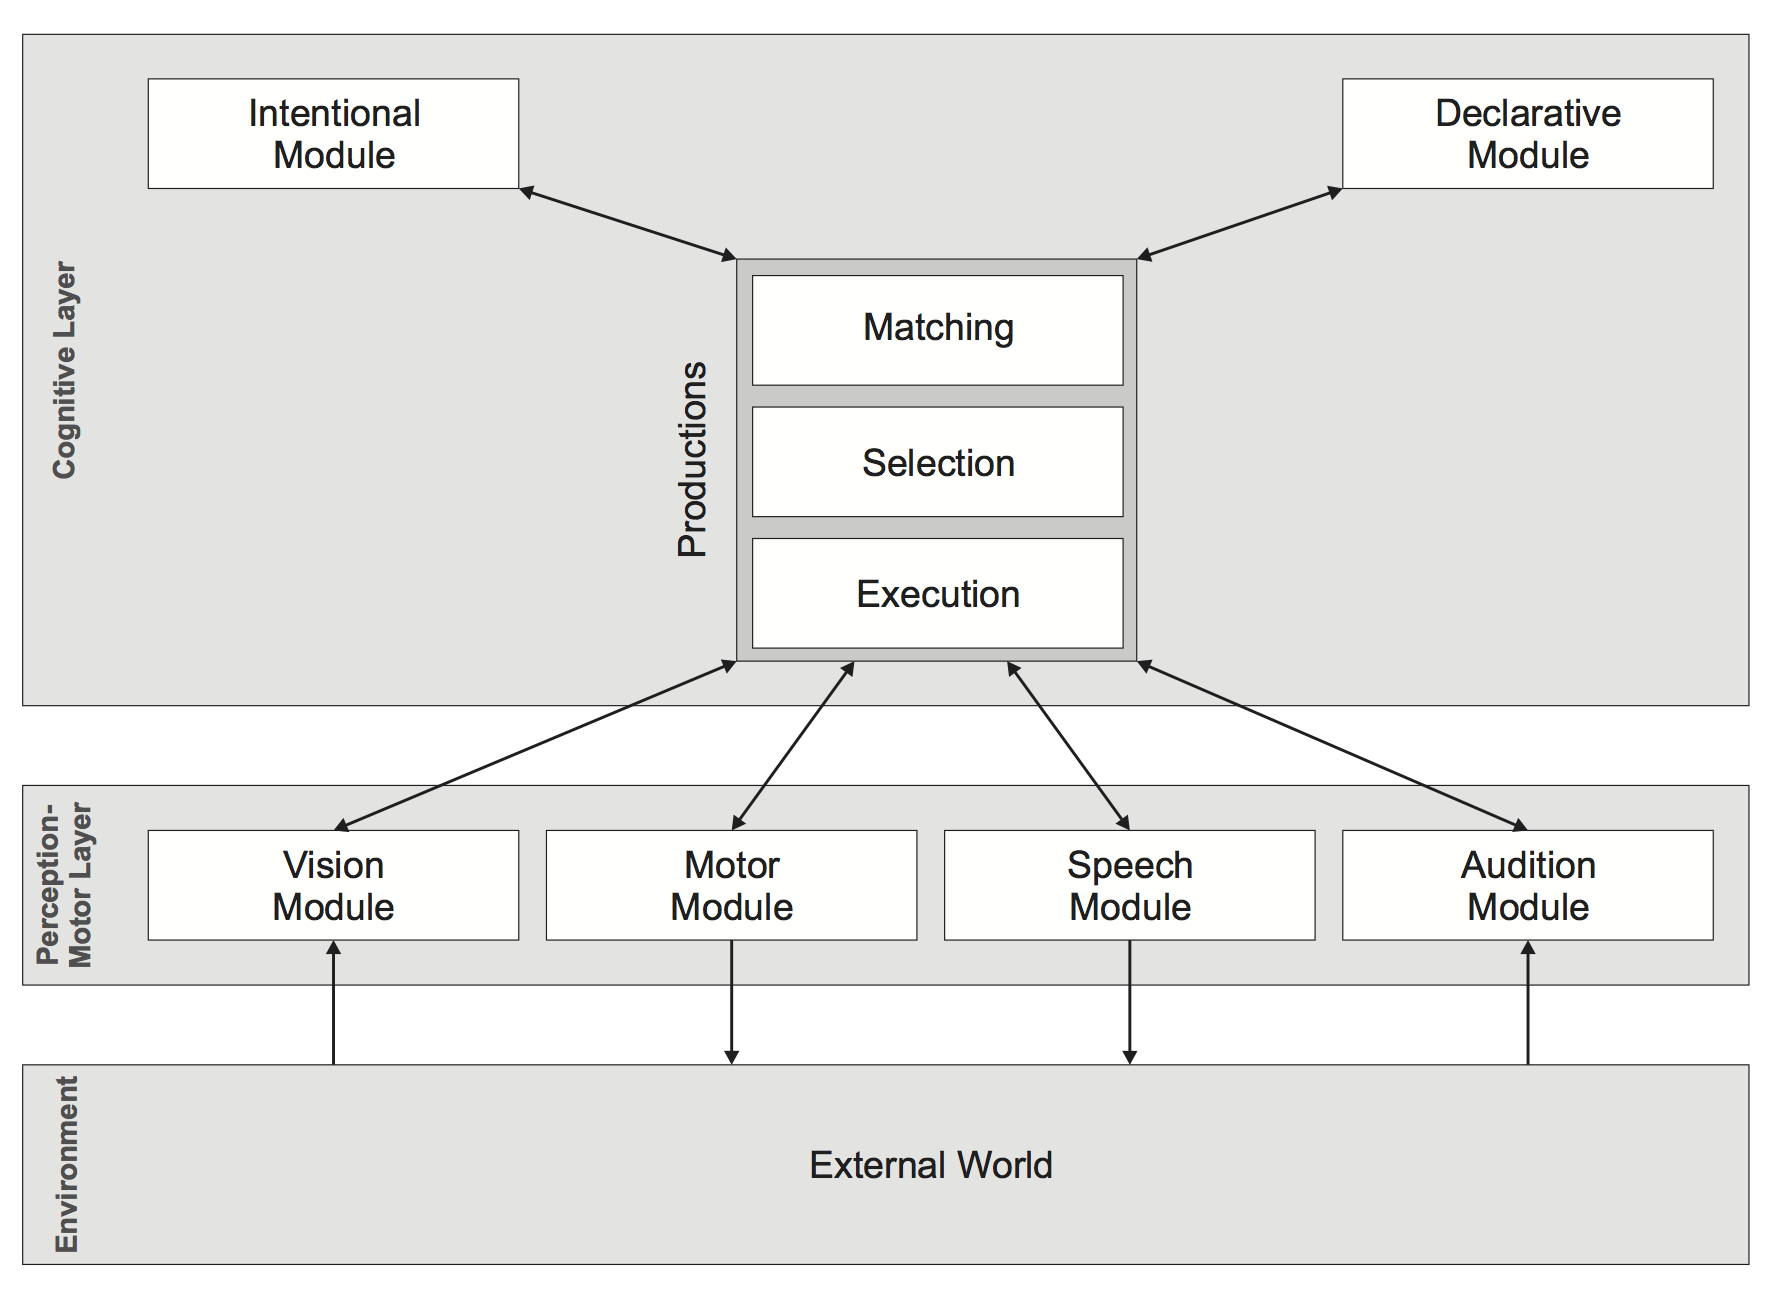
\includegraphics[width=0.85\textwidth]{act_r.png}
    \caption{Overview of the ACT-R high level architecture (from \cite{actr_4}).}
    \label{fig:act_r_1}
\end{figure}

The architecture can be generally described as two distinct modules: a \textit{perceptual-motor} layer and a \textit{cognitive} layer, as presented in Figure~\ref{fig:act_r_1}. The perceptual-motor module corresponds to the interface of the cognition with the environment (which plays a key role in ACT-R), being comprised of sub-modules such as vision and motor actions. The cognitive layer is focused on memory, which can be divided into two different categories: \textit{declarative} (consisting of factual knowledge and goals - e.g. \textit{"The maximum driving speed in a typical UK motorway is 70 mph"} or \textit{"Try get to point B"}) and \textit{procedural} (consisting of rules/procedures - e.g. \textit{"If the lead vehicle is going slowly, attempt an overtake"}) \cite{actr_4}. Furthermore, declarative memory is composed of \textit{chunks}, which are smaller pieces of information divided into categories or attributes that form more complex memories. In the example \textit{"The maximum driving speed in a typical UK motorway is 70 mph"}, \texttt{maximum driving speed in a typical UK motorway} is a category, whereas \texttt{70 mph} is an attribute. Another possible attribute for this category could be \texttt{112 km/h} (since $70 mph = 112 km/h$).

\section{Integrated Driver Modelling in ACT-R}
\label{sec:salvucci}

The first integrated approaches to this problem, proposed in \cite{older_1,older_2,older_3}, rely on modelling human behaviour through continuous controllers and specifically engineered frameworks. However, these methods lack the human behaviour variability attributed to the discrete nature of the control actions performed by the drivers. With this in mind, in \cite{salvucci_0} Salvucci \textit{et al.} proposed a proof-of-concept of the introduction of human constrains in the driver model through the use of the cognitive architecture ACT-R. In \cite{salvucci_1}, Salvucci proposed an updated version of the human driver model initially introduced in \cite{salvucci_0}, which was improved using the advances in ACT-R (the model uses version 5.0 of the architecture) and re-designed elements (e.g. lane changing behaviour or distraction) resulting from validation performed by empirical studies.

The model Salvucci introduced in \cite{salvucci_1} was developed with a specific scenario in mind: \textit{"(...) driving a standard midsize vehicle on a multilane highway with moderate traffic"} \cite{salvucci_1}. It consists of three distinct modules interacting in a sequential way: \textbf{control}, \textbf{monitoring}, and \textbf{decision making}. A high level schematic of the model can be found in Figure~\ref{fig:high_level_salvucci}.

\begin{figure}[h]
    \centering
    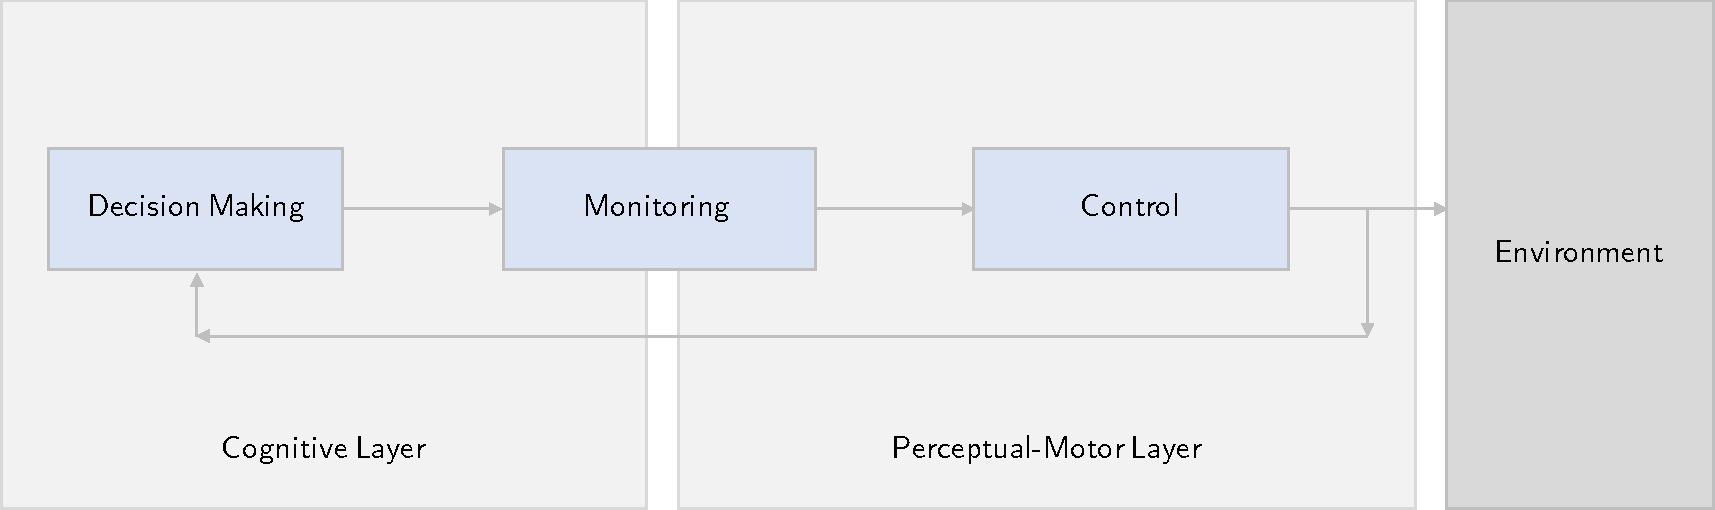
\includegraphics[width=1\textwidth]{high_level_salvucci.pdf}
    \caption{High level representation of the architecture presented in \cite{salvucci_1}.}
    \label{fig:high_level_salvucci}
\end{figure}

The \textbf{control} component manages both the lower level perception cues and the physical manipulation of the vehicle (e.g. steering, accelerating or breaking). The module can be divided into lateral (i.e. steering) and longitudinal (i.e. speed) control, each modelled by a separate control law. 

The lateral control is determined by the existence of two artefacts that the driver obtains using lower level perception cues: the \textit{near point} and the \textit{far point}. In this model,  \textit{"the near point represents the vehicle’s current lane position, used to judge how close the vehicle is to the center of the roadway (...) [and] is characterized as a point in the center of the near lane visible in front of the vehicle, set at a distance of 10 m from the vehicle’s center"} while \textit{"the far point indicates the curvature of the upcoming roadway, used to judge what the driver should execute to anticipate the upcoming curvature and remain in the current lane} \cite{salvucci_1}. At any cycle $i > 0$, the model works by using perception to determine the visual angles $\theta_{near}^{(i)}$ and $\theta_{far}^{(i)}$ and calculates:

\begin{equation}
\begin{split}
	\Delta \theta_{near} & = \theta_{near}^{(i)} - \theta_{near}^{(i-1)} \\
	\Delta \theta_{far} & = \theta_{far}^{(i)} - \theta_{far}^{(i-1)}
\end{split}
\end{equation}

The control law for the steering angle $\varphi$ can be defined as:

\begin{equation}
	\Delta \varphi = k_{far} \Delta \theta_{far} + k_{near} \Delta \theta_{near} + k_I \min{(\theta_{near}^{(i)}, \theta_{\max})} \Delta t
\end{equation}

with $k_{far}$, $k_{near}$ and $k_{I}$ defined as in \cite{salvucci_1}.

The process for the longitudinal control is very similar. At any cycle $i > 0$, the model starts by encoding the position of the lead vehicle and calculating the time headway $thw_{car}^{(i)}$ to it. It then computes:

\begin{equation}
	\Delta thw_{car} = thw_{car}^{(i)} - thw_{car}^{(i-1)}
\end{equation}

The control law for the linear acceleration $\psi$ can be written as:

\begin{equation}
	\Delta \psi = k_{car} \Delta thw_{car} + k_{follow} (thw_{car} - thw_{follow})\Delta t
\end{equation}

with $k_{car}$, $k_{follow}$ and $thw_{car}$ defined as in \cite{salvucci_1}.

These control laws can be applied in order to model the behaviour of the driver in terms of lane keeping and curve negotiation, and generalise to lane changing actions in a straightforward manner. In order to initiate a lane change, the driver just starts following the near and far points of the destination lane instead of the current lane, as Salvucci and Liu presented in \cite{older_3}.

The \textbf{monitoring} component maintains situational awareness through the awareness of the position of other vehicles around the driver's vehicle. It accomplishes this through a random-sampling, with probability $p_{monitor}$, of one of four areas: either the left or right lane, and either forward or backward (with equal probability). After deciding which area to sample (if any), the model uses visual perception to determine whether a vehicle is present or not. If it is, the distance, lane and direction are saved in ACT-R's declarative memory. The value of $p_{monitor}$ is defined in \cite{salvucci_1}.

Finally, the \textbf{decision making} module uses the information gathered in the monitoring and control stage (if any is available) to determine which tactical decision should be taken. In this model, the decision corresponds to determining when and where a lane change should occur. Salvucci describes this process in \cite{salvucci_1} as: \textit{"If the driver’s vehicle is in the right lane, the model checks the current time headway to the lead vehicle (if any); if the lead car time headway drops below a desired time headway $thw_{pass}$, the model decides to change lanes to pass the vehicle. If the driver vehicle is in the left lane, the model checks instead simply for the presence of a lead vehicle. If there is a lead vehicle, the model remains in the left lane (because this vehicle is also passing other vehicles); otherwise it decides to [try to] change lanes to return to the right lane"}. This process is summarised in the flowchart presented in Figure~\ref{fig:flowchart_dm}, and the value of $thw_{pass}$ is defined in \cite{salvucci_1}.

\begin{figure}[h]
    \centering
    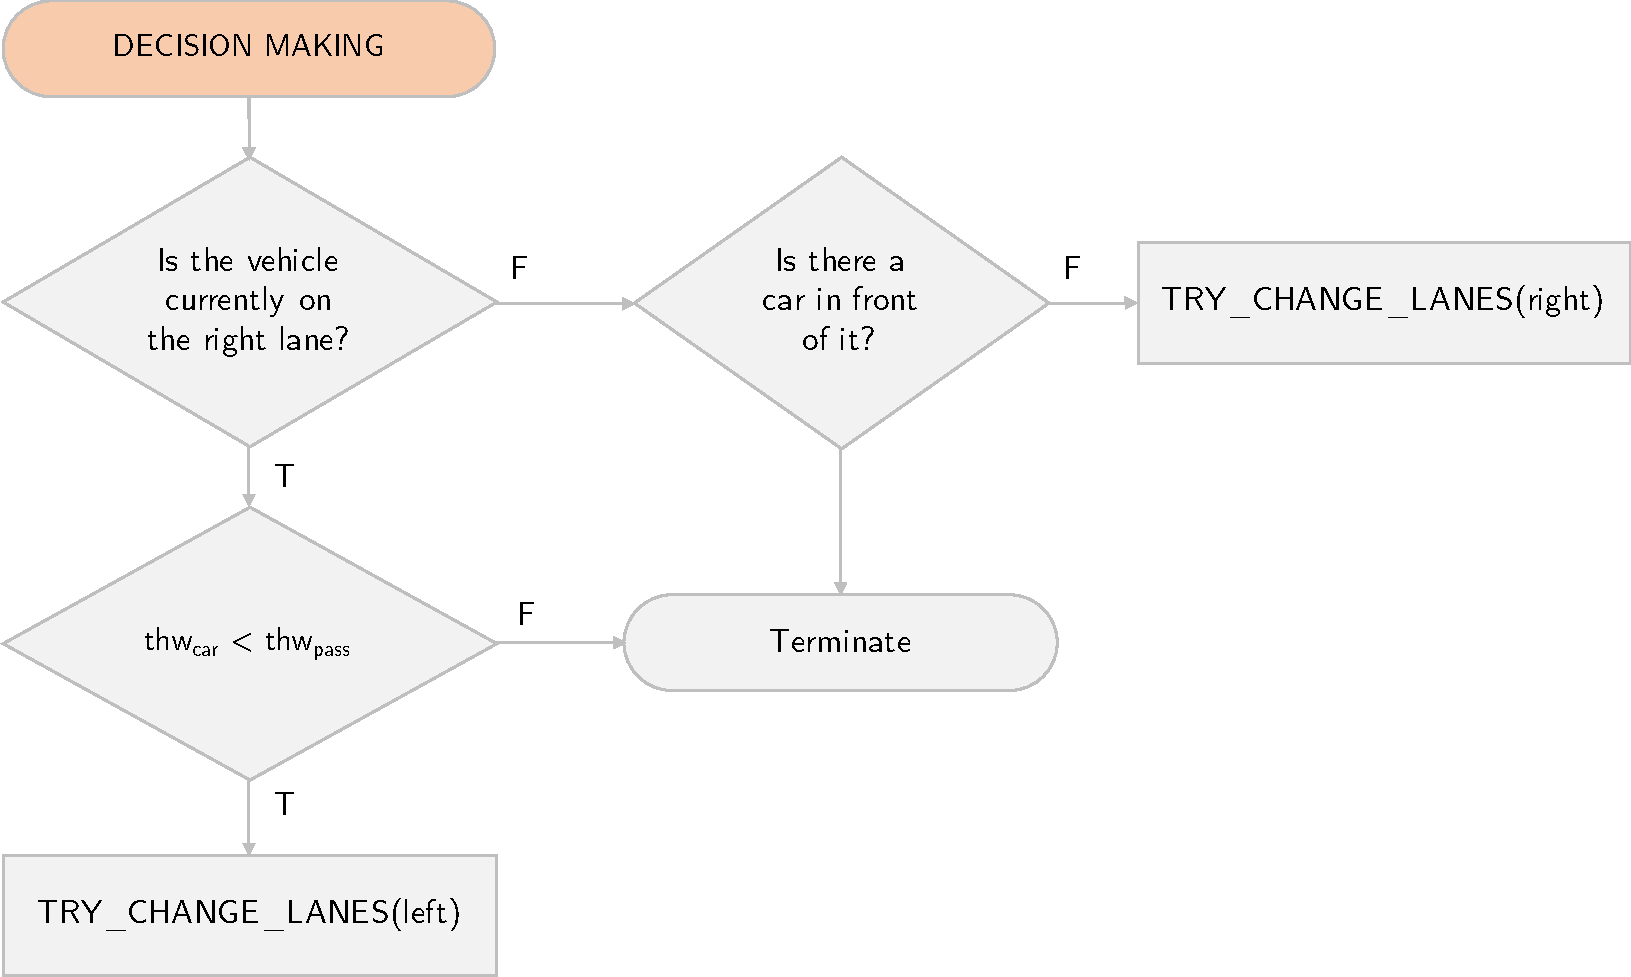
\includegraphics[width=1\textwidth]{flowchart_dm.pdf}
    \caption{Flowchart of part of the decision making process of the model.}
    \label{fig:flowchart_dm}
\end{figure}

Even after this decision to change lanes is taken, the model must then determine whether it is actually safe to do so. In order to verify that it is, the model initially attempts to recall, from the declarative memory, the nearest vehicle to it in the destination lane. If one is recalled at a distance closer than $d_{safe}$, then the change is aborted. If not, then the vehicle performs a safety monitoring of the destination lane. If this monitoring does not observe a vehicle at a distance closer than $d_{safe}$, then the vehicle initiates the execution of the lane change. The parameter $d_{safe}$ is as defined in \cite{salvucci_1}.

\section{Probabilistic Model Checking}

Model checking is a formal verification technique consisting of the process of automatically verifying, through exhaustive search, whether a model meets a given specification \cite{bk08}. A model in this context is considered to be a labelled finite state-transition system, with states corresponding to configurations of the system and transitions between states representing the evolution between the said configurations.

Probabilistic model checking is a generalisation of model checking for the automated verification of systems that exhibit probabilistic behaviour \cite{fknp11, bk08}. It should be noted that this is not to be confused with \textit{probabilistic verification}, which amounts to partial state-space exploration \cite{bk08}. Within this section, important concepts of probabilistic model checking related to modelling of systems, and verification and synthesis of models will be explained in detail.

\subsection{Markov Chains and Decision Processes}
\label{sec:dtmcs_mdps}

Probabilistic model checking begins with the appropriate modelling of the system in a stochastic finite state-transition representation. There are several ways to do this according to the type of system to be modelled. 

In \textit{discrete-time Markov Chains} (DTMCs), all choices (i.e. transitions) are probabilistic \cite{bk08}. While this is useful in some cases, others require nondeterminism, which is where \textit{Markov Decision Processes} (MDPs) come in. In MDPs, nondeterministic probabilistic choices coexist. Essentially, a DTMC is an MDP with a uniquely determined probabilistic distribution \cite{bk08}. Both DTMCs and MDPs can be augmented with reward structures, which correspond to real positive values that can be interpreted as bonuses or costs \cite{bk08}.

The formal definitions of DTMCs, MDPs and reward structures follow (adapted from \cite{bk08, fknp11, kp07}).

{\begin{defi}
{\setlength{\parskip}{2em}
\textbf{Discrete-time Markov Chain (DTMC)}\vspace{1em}\\}
{\setlength{\parskip}{1em} 

A \textit{discrete-time Markov chain} is a tuple $\mathcal{M} = (S, \mathbf{P}, p_{init}, AP, L)$ such that:
\begin{itemize}
	\item $S$ is a countable, non-empty set of states
	\item $\mathbf{P}: S \times S \to [0,1]$ is a transition probability function such that for all states $s \in S$:
		\begin{equation}
			\sum_{s' \in S} \mathbf{P}(s,s') = 1
		\end{equation}
	\item $p_{init}: S \to [0,1]$ is the initial state distribution, such that:
		\begin{equation}
			\sum_{s \in S} p_{init}(s) = 1
		\end{equation}
	\item $AP$ is a set of atomic propositions and $L: S \to 2^{AP}$ is a labelling function. 
\end{itemize}

$\mathcal{M}$ is denoted \textit{finite} if $S$ and $AP$ are finite sets.
}
\end{defi}}

{\begin{defi}
{\setlength{\parskip}{2em}
\textbf{Markov Decision Process (MDP)}\vspace{1em}\\}
{\setlength{\parskip}{1em} 

A \textit{Markov decision process} is a tuple $\mathcal{M} = (S, Act, \mathbf{P}, p_{init}, AP, L)$ such that:
\begin{itemize}
	\item $S$ is a countable, non-empty set of states
	\item $Act$ is a set of actions
	\item $\mathbf{P}: S \times Act \times S \to [0,1]$ is a transition probability function such that for all states $s \in S$ and actions $\alpha \in Act$:
		\begin{equation}
			\sum_{s' \in S} \mathbf{P}(s,\alpha,s') \in \{0,1\}
		\end{equation}
	\item $p_{init}: S \to [0,1]$ is the initial state distribution, such that:
		\begin{equation}
			\sum_{s \in S} p_{init}(s) = 1
		\end{equation}
	\item $AP$ is a set of atomic propositions and $L: S \to 2^{AP}$ is a labelling function. 
\end{itemize}

An action $\alpha \in Act$ is enabled in a state $s$ if, and only if, $\sum_{s' \in S} \mathbf{P}(s,\alpha,s') = 1$. Let $Act(s)$ denote the set of actions enabled in a state $s$. It must be that for all states $s \in S$, $Act(s) \neq \emptyset$.
}
\end{defi}}

{\begin{defi}
{\setlength{\parskip}{2em}
\textbf{Reward Structures for DTMCs and MDPs}\vspace{1em}\\}
{\setlength{\parskip}{1em} 
A \textit{reward structure} for a discrete-time Markov chain $\mathcal{M} = (S, \mathbf{P}, p_{init}, AP, L)$ is a tuple $\mathcal{C} = (\rho, \iota)$ such that:
\begin{itemize}
	\item $\rho: S \to \mathbb{R}_{\geq 0}$ is a state reward function
	\item $\iota: S \times S \to \mathbb{R}_{\geq 0}$ is a transition reward function
\end{itemize}
	
A \textit{reward structure} for a Markov decision process $\mathcal{M} = (S, Act, \mathbf{P}, p_{init}, AP, L)$ is a tuple $\mathcal{C} = (\rho, \iota)$ such that:
\begin{itemize}
	\item $\rho: S \to \mathbb{R}_{\geq 0}$ is a state reward function
	\item $\iota: S \times Act \to \mathbb{R}_{\geq 0}$ is an action reward function
\end{itemize}
}
\end{defi}}

There are some additional concepts related to DTMCs and MDPs which are relevant to the understanding of temporal logics and model checking. These are the concepts of paths in Markov chains or decision processes, and adversary in a Markov decision process (adapted from \cite{bk08, fknp11}).

{\begin{defi}
{\setlength{\parskip}{2em}
\textbf{Paths in DTMCs and MDPs}\vspace{1em}\\}
{\setlength{\parskip}{1em} 
An \textit{(infinite) path} $\pi$ in a discrete-time Markov chain $\mathcal{M} = (S, \mathbf{P}, p_{init}, AP, L)$ is defined as an infinite sequence of states $\pi = s_0 \to s_1 \to s_2 ...$ (also written as $\pi = s_0s_1s_2...$) such that $\forall i \geq 0: \mathbf{P}(s_i, s_{i+1}) > 0$.

A \textit{finite path} $\rho$ in the discrete-time Markov chain $\mathcal{M}$ is defined as the prefix of an infinite path $\pi$, $\rho = s_0 \to s_1 \to ... \to s_n$ for $n > 0$.

An \textit{(infinite) path} $\pi$ in a Markov decision process $\mathcal{M} = (S, Act, \mathbf{P}, p_{init}, AP, L)$ is defined as an infinite sequence of states and actions $\pi = s_0 \xrightarrow{a_0} s_1 \xrightarrow{a_1} s_2 ...$ (also written as $\pi = s_0a_0s_1a_1s_2...$) such that $\forall i \geq 0: \mathbf{P}(s_i, a_i, s_{i+1}) > 0$.

A \textit{finite path} $\rho$ in the Markov decision process $\mathcal{M}$ is defined as the prefix of an infinite path $\pi$, $\rho = s_0 \xrightarrow{a_0} s_1 \xrightarrow{a_1} ... \xrightarrow{a_{n-1}} s_n$ for $n > 0$.

In both Markov chains and decision processes, the set of all infinite paths is denoted by $Paths(\mathcal{M})$, while the set of finite paths is denoted by $Paths_{fin}(\mathcal{M})$
}
\end{defi}}

{\begin{defi}
{\setlength{\parskip}{2em}
\textbf{Adversary (alternatively Strategy or Scheduler)}\vspace{1em}\\}
{\setlength{\parskip}{1em} 
An \textit{adversary} for an MDP $\mathcal{M} = (S, Act, \mathbf{P}, p_{init}, AP, L)$ is a function $\sigma: S^+ \to Act$ such that $\sigma(s_0s_1...s_n) \in Act(s_n)$ for all $s_0s_1...s_n \in S^+$.

An adversary $\sigma$ is called memoryless if, and only if, for any $\pi_1 = s_0s_1...s_n$ and $\pi_2 = s'_0s'_1...s_n$ it is true that $\sigma(\pi_1) = \sigma(\pi_2) = \sigma(s_n)$.
}
\end{defi}}

\subsection{Temporal Logics}
\label{sec:temp_logics}

In order to verify properties in models, there needs to be a way of expressing them formally and unequivocally. While some reachability and reward-based properties come directly from the definition of DTMCs, MDPs and reward structures \cite{fknp11}, more interesting and complex properties require the use of a temporal logic. A propositional temporal logic is essentially an extension of propositional logic by temporal operators \cite{bk08}. In this context, one can consider time as being \textit{linear} or \textit{branching}. In linear time, at every moment in time there must only exist a single successor moment, whereas from the branching perspective, there may exist multiple ones, forming a tree-like structure of alternatives. Linear Temporal Logic (LTL) is a temporal logic which assumes the first, while Computation Tree Logic (CTL) is based on the branching perspective. Probabilistic Computational Tree Logic (PCTL) is an extension of CTL that takes into account a probabilistic operator.

Given the definition of a path in an MC and MDP, it is possible to define the syntax for LTL, CTL and PCTL (adapted from \cite{bk08, fknp11}).

{\begin{defi}
{\setlength{\parskip}{2em}
\textbf{Syntax and Semantics of LTL}\vspace{1em}\\}
{\setlength{\parskip}{1em} 
An \textit{LTL formulae} $\varphi$ over a set of atomic propositions $AP$ can formed according to the following grammar:

\begin{equation}
	\varphi ::= \text{\texttt{true}} \bigmid a \bigmid \varphi_1 \wedge \varphi_2 \bigmid \neg \varphi \bigmid \text{X} \varphi \bigmid \varphi_1 \text{ U } \varphi_2
\end{equation}

where $a \in AP$, X is the next operator and U is the until operator as defined below for Markov chains and decision processes.

For a given path $\pi = s_0s_1s_2...$ in a discrete-time Markov chain $\mathcal{M} = (S, \mathbf{P}, p_{init}, AP, L)$ (generalising trivially to a Markov decision process):
\begin{itemize}
	\item $\pi \models $\texttt{true} always.
	\item $\pi \models a$ if, and only if, $a \in L(s_0)$.
	\item $\pi \models \varphi_1 \wedge \varphi_2$ if, and only if, $\pi \models \varphi_1 \wedge \pi \models \varphi_2$.
	\item $\pi \models \neg \varphi$ if, and only if, $\pi \not\models \varphi$.
	\item $\pi \models \text{X}\varphi$ if, and only if, $s_1s_2... \models \varphi$.
	\item $\pi \models \varphi_1\text{ U }\varphi_2$ if, and only if:
	 \begin{equation}
	 	\exists i \geq 0 \text{ s.t. } (s_is_{i+1}... \models \varphi_2) \wedge (\forall j < i: s_js_{j+1}... \models \varphi_1)
	\end{equation}
\end{itemize}

The operator F (eventually) can also be defined as:

\begin{equation}
	\text{F} \varphi = \text{\texttt{true}} \text{ U } \varphi
\end{equation}

}
\end{defi}}

It can be noticed that, as a result of the linear time consideration in LTL, all the formulas are taken over paths. This is not the case in CTL which can have both path and state formulae, as shown below.

{\begin{defi}
{\setlength{\parskip}{2em}
\textbf{Syntax and Semantics of CTL}\vspace{1em}\\}
{\setlength{\parskip}{1em} 
A \textit{CTL state formulae} $\Phi$ over a set of atomic propositions $AP$ can formed according to the following grammar:

\begin{equation}
	\Phi ::= \text{\texttt{true}} \bigmid a \bigmid \Phi_1 \wedge \Phi_2 \bigmid \neg \Phi \bigmid \text{E} \varphi \bigmid \text{A} \varphi
\end{equation}

where $a \in AP$ and $\varphi$ is a path formula.

For a given state $s \in S$ in a discrete-time Markov chain $\mathcal{M} = (S, \mathbf{P}, p_{init}, AP, L)$ (generalising trivially to a Markov decision process):
\begin{itemize}
	\item $s \models $\texttt{true} always.
	\item $s \models a$ if, and only if, $a \in L(s)$.
	\item $s \models \Phi_1 \wedge \Phi_2$ if, and only if, $s \models \Phi_1 \wedge s \models \Phi_2$.
	\item $s \models \neg \Phi$ if, and only if, $s \not\models \Phi$.
	\item $s \models \text{E} \varphi$ if, and only if, $\exists \pi \in Paths(s): \pi \models \varphi$.
	\item $s \models \text{A} \varphi$ if, and only if, $\forall \pi \in Paths(s): \pi \models \varphi$
\end{itemize}

A \textit{CTL path formulae} $\varphi$ over a set of atomic propositions $AP$ can formed according to the following grammar:

\begin{equation}
	\varphi ::= \text{X} \Phi \bigmid \Phi_1 \text{ U } \Phi_2
\end{equation}

where $a \in AP$ and $\Phi$ is a state formula.

For a given path $\pi = s_0s_1s_2...$ in a Markov chain $\mathcal{M} = (S, \mathbf{P}, p_{init}, AP, L)$ (generalising trivially to a Markov decision process):
\begin{itemize}
	\item $\pi \models \text{X}\Phi$ if, and only if, $s_1 \models \Phi$.
	\item $\pi \models \Phi_1\text{ U }\Phi_2$ if, and only if:
	 \begin{equation}
	 	\exists i \geq 0 \text{ s.t. } (s_i \models \Phi_2) \wedge (\forall j < i: s_j \models \Phi_1)
	\end{equation}
\end{itemize}

It is also possible to define the operators F (eventually) and G (globally) as:

\begin{equation}
\begin{aligned}
	\text{F} \Phi & = \text{\texttt{true}} \text{ U } \Phi \\
	\text{G} \Phi & = \neg \text{E} (\neg \Phi)
\end{aligned}
\end{equation}

}
\end{defi}}

{\begin{defi}
{\setlength{\parskip}{2em}
\textbf{Syntax and Semantics of PCTL}\vspace{1em}\\}
{\setlength{\parskip}{1em} 
A \textit{PCTL state formulae} $\Phi$ over a set of atomic propositions $AP$ can formed according to the following grammar:

\begin{equation}
	\Phi ::= \text{\texttt{true}} \bigmid a \bigmid \Phi_1 \wedge \Phi_2 \bigmid \neg \Phi \bigmid \mathbb{P}_{\triangleright p} (\varphi)
\end{equation}

where $a \in AP$, $p \in [0,1]$, $\triangleright \in \{>, <, \geq, \leq\}$ is a probability bound and $\varphi$ is a path formula.

For a given state $s \in S$ in a discrete-time Markov chain $\mathcal{M} = (S, \mathbf{P}, p_{init}, AP, L)$ (generalising trivially to a Markov decision process):
\begin{itemize}
	\item $s \models $\texttt{true} always.
	\item $s \models a$ if, and only if, $a \in L(s)$.
	\item $s \models \Phi_1 \wedge \Phi_2$ if, and only if, $s \models \Phi_1 \wedge s \models \Phi_2$.
	\item $s \models \neg \Phi$ if, and only if, $s \not\models \Phi$.
	\item $s \models \mathbb{P}_{\triangleright p} (\varphi)$ if, and only if, $P_s (\pi \in Paths(s): \pi \models \varphi) \triangleright p$ (that is, the probability, from state $s$, that $\varphi$ is true for an outgoing path satisfies $\triangleright p$).
\end{itemize}

A \textit{PCTL path formulae} $\varphi$ over a set of atomic propositions $AP$ can formed according to the following grammar:

\begin{equation}
	\varphi ::= \text{X} \Phi \bigmid \Phi_1 \text{ U}^{\leq k}\, \Phi_2 \bigmid \Phi_1 \text{ U } \Phi_2
\end{equation}

where $a \in AP$, $k \in \mathbb{N}$ and $\Phi$ is a state formula.

For a given path $\pi = s_0s_1s_2...$ in a discrete-time Markov chain $\mathcal{M} = (S, \mathbf{P}, p_{init}, AP, L)$ (generalising trivially to a Markov decision process):
\begin{itemize}
	\item $\pi \models \text{X}\Phi$ if, and only if, $s_1 \models \Phi$.
	\item $\pi \models \Phi_1\text{ U}^{\leq k}\, \Phi_2$ if, and only if:
	 \begin{equation}
	 	\exists i \leq k \text{ s.t. } (s_i \models \Phi_2) \wedge (\forall j < i: s_j \models \Phi_1)
	\end{equation}
	\item $\pi \models \Phi_1\text{ U }\Phi_2$ if, and only if:
	 \begin{equation}
	 	\exists i \geq 0 \text{ s.t. } (s_i \models \Phi_2) \wedge (\forall j < i: s_j \models \Phi_1)
	\end{equation}
\end{itemize}

Similarly to CTL, it is possible to define the operators F (eventually) and G (globally) as:

\begin{equation}
\begin{aligned}
	\text{F} \Phi & = \text{\texttt{true}} \text{ U } \Phi \\
	\text{G} \Phi & = \neg \text{E} (\neg \Phi)
\end{aligned}
\end{equation}

}
\end{defi}}

While PCTL path formulas are defined above, it should be mentioned that all PCTL formulas are state formulas, and that path formulas should only appear inside the probabilistic operator. 

In relation to the probabilistic operator in PCTL, the generalisation from the Markov chain to the Markov decision process can be done using the concept of adversary (also denoted strategy or scheduler), initially introduced in Section~\ref{sec:dtmcs_mdps}. In the case of an MDP, the operator $\mathbb{P}_{\triangleright p}$ should be interpreted under the following semantics:

\begin{equation}
	s \models \mathbb{P}_{\triangleright p} (\varphi) \text{ if, and only if, } \forall \sigma \in Adv: Pr^{\sigma}_s (\pi \in Paths^{\sigma}(s): \pi \models \varphi) \triangleright p
\end{equation}

that is, the probability, from state $s$, that $\varphi$ is true for an outgoing path satisfies $\triangleright p$ for all adversaries $\sigma \in Adv$ (with $Adv$ constituting the set of all adversaries that the MDP admits).

\subsection{PRISM Language}

PRISM is a probabilistic model checking tool developed in cooperation between the Universities of Oxford and Birmingham \cite{prism}. It was one of the first tools within stochastic model checking to be released and it is currently maintained by David Parker. In order to use PRISM (and other alternative model checking techniques), it is essential to be able to specify the model. To achieve this, the team behind PRISM developed the PRISM Language, initially described in \cite{prism_1}.

A model described in the PRISM Language (typically a \texttt{.pm}, \texttt{.nm} or \texttt{.prism} text file) should contain a keyword that indicates the kind of model to expect. For example, the keyword \texttt{dtmc} indicates the model is a DTMC (discrete-time Markov chain) and \texttt{mdp} indicates a MDP (Markov decision process).

The PRISM language uses two different basic components to define a model \textit{modules} and \textit{variables}. A module is composed of a set of local variables whose behaviour is described by \textit{commands}. A general command is of the form:

{\vspace{1em}
\begin{lstlisting}
[] guard -> prob_1: update_1 + ... + prob_n: update_n;
\end{lstlisting}
}

where \textit{guard} is a boolean expression over the variables, \textit{prob\_i} is the probability that \textit{update\_i} will be taken (with $\sum_i \text{prob\_i} = 1$) and \textit{update\_i} is the the new value of local and/or global variables if the guard is true and a transition is taken to this configuration.

A state of the module is defined as a configuration of its local variables, and a state of the model is a configuration of the states of all modules which compose it and the global variables.

In Listing \ref{lst:example}, an example of a simple MDP model described in PRISM Language is shown. This example is comprised of two modules, \texttt{M1} and \texttt{M2}, each with their own local variables, and no global variables are declared. It should be noted that the variables in PRISM Language should either be integers (\texttt{int}) or booleans (\texttt{bool}) and can be initialised by specifying \texttt{init} after the initial declaration. Due to the fact that we are dealing with finite models, the integers must be in a finite range as well.

{\vspace{1em}
\begin{lstlisting}[caption={Example of a simple MDP model from \cite{prism_example}},captionpos=b,label={lst:example}]
// Example 1 (modified)
// Two process mutual exclusion

mdp

module M1

    x : [0..2] init 0;

    [] x=0 -> 0.8:(x'=0) + 0.2:(x'=1);
    [] x=1 & y!=2 -> (x'=2);
    [] x=2 -> 1:(x'=2);
    [] x=2 -> 1:(x'=0);

endmodule

module M2

    y : [0..2] init 0;

    [] y=0 -> 0.8:(y'=0) + 0.2:(y'=1);
    [] y=1 & x!=2 -> (y'=2);
    [] y=2 -> 1:(y'=2);
    [] y=2 -> 1:(y'=0);

endmodule
\end{lstlisting}
}

Models in the PRISM Language can also include \textit{formulas}, which are expressions that avoid repetition of code, and \textit{labels}, which are boolean expressions that identify sets of states of interest.

It is also possible to define rewards structures using the following convention:

\begin{minipage}{\linewidth}
{\vspace{1em}
\begin{lstlisting}
rewards "name"
    guard: state_reward;
    ...
    [action] guard: transition_reward;
    ...
endrewards
\end{lstlisting}
}
\end{minipage}

where the \textit{guards} are similarly defined as before, but the distinction between state and transition rewards is defined by the \textit{action} (which may be empty).

\subsection{Model Checking in DTMCs and MDPs}

After the description of the model using a language such as the PRISM Language, it is possible to verify properties on the said model. These properties can be of different types according to the model and the model checking tool chosen. 

In this dissertation, the models built will be represented through discrete-time Markov chains and Markov decision processes, so the properties of interest tend to be best expressed in the temporal logics LTL or PCTL. The PRISM model checker is one of the tools which allows a user to import a text file with the probabilistic model, build it and verify LTL and PCTL properties on it \cite{prism}. Another tool used for this purpose is the Storm model checker \cite{storm}. Each of these tools has it strengths and weaknesses. PRISM is an extremely robust tool, with lots of options in terms of engines to perform the required calculations, and a graphical interface. Storm is a relatively recent tool which builds on top of some of PRISM's features and introduces new ones, such as an optimised Sparse engine (a great advantage when dealing with models with a small state space) and conditional properties in DTMCs \cite{storm}. However, it does not provide a graphical interface and is limited in terms of capabilities and I/O. Due to the fact that Storm builds on top of PRISM, it uses the PRISM Language for model input and the properties are specified using the same convention.

In order to illustrate properties, consider the example of Listing~\ref{lst:example}. A PCTL property in this case could be defined as:

\begin{minipage}{\linewidth}
{\vspace{1em}
\begin{lstlisting}
P>=0.5 [F x = 2]
\end{lstlisting}
}
\end{minipage}

This property can be interpreted as \textit{"with probability greater or equal to 0.5, eventually the model reaches a state where }\texttt{x = 2}\textit{"}. Building the model and verifying the property yields the value \texttt{false}, which means that, according to this model, there exists at least one adversary under which this property is not satisfied. Both PRISM and Storm allow for quantitative probabilistic properties as well. These properties take different formats in DTMCs and MDPs, as presented below.

\begin{minipage}{\linewidth}
{\vspace{1em}
\begin{lstlisting}
// DTMC
P=? [F x = 2]

// MDP
Pmin=? [F x = 2]
Pmax=? [F x = 2]
\end{lstlisting}
}
\end{minipage}

Instead of returning a boolean value of satisfaction, these return the actual values of the probabilities of the properties being satisfied. They are, therefore, extremely useful metrics for model comparison. For the case of the DTMC, due to the fact that there is no nondeterminism, the probability of a path is uniquely defined (as seen in Section~\ref{sec:temp_logics}), and thus can be expressed simply as \texttt{P=?}. For MDPs, this is not the case. In order to verify the probabilistic operator $\mathbb{P}_{\triangleright p}$ on the path formula $\varphi$, a model checker needs to calculate the following quantities:

\begin{equation}
\begin{aligned}
	p_{\max, s} (\varphi) & = \sup_{\sigma \in Adv} P^{\sigma}_s (\varphi) \\
	p_{\min, s} (\varphi) & = \inf_{\sigma \in Adv} P^{\sigma}_s (\varphi)
\end{aligned}
\end{equation}

where $P^{\sigma}_s (\varphi) = Pr^{\sigma}_s (\pi \in Paths^{\sigma}(s): \pi \models \varphi)$.

Therefore, PRISM and Storm allow users to access these values by writing properties using \texttt{Pmax} and \texttt{Pmin} (boolean or quantitative). 

Storm allows for conditional probability properties of the type:

\begin{minipage}{\linewidth}
{\vspace{1em}
\begin{lstlisting}
P=? [ F x=2 || F y=2 ]
\end{lstlisting}
}
\end{minipage}

This property can be interpreted as \textit{"what is the probability that the model eventually reaches the state} \texttt{x = 2}\textit{, given that it eventually reaches the state} \texttt{y = 2}\textit{"}. These properties, in DTMCs, correspond simply to the application of Bayes' theorem of conditional probability, which states that:

\begin{equation}
	P_s (\varphi_1 \bigmid \varphi_2) = \frac{P_s (\varphi_1 \wedge \varphi_2)}{P_s (\varphi_2)}
\end{equation}

For $P_s (\varphi_2) \neq 0$. It must be emphasised that this is \textbf{not} the case for MDPs, where the existence of multiple adversaries complicates the calculations of conditional probabilities.

This does not mean that it is not possible to reason over conditional probabilities in MDPs. For some specific scenarios, it is possible to obtain meaningful bounds which allow comparisons between the ones obtained in DTMCs and MDPs. One of those scenarios is defined in the proposition below, with the proof following it.

\begin{proposition}
Consider a Markov decision process $\mathcal{M} = (S, Act, \mathbf{P}, p_{init}, AP, L)$ which admits adversaries $\sigma \in Adv$. Let $\varphi_1, \varphi_2$ be two PCTL path formulas, such that, for any path $\pi \in Paths(s)$: $\pi \models \varphi_1 \Rightarrow \pi \models \varphi_2$. Assume as well that:

\begin{equation}
	\sigma' \in \arg\sup_{\sigma \in Adv} P^{\sigma}_s (\varphi_1 \bigmid \varphi_2)
\end{equation}

And that:

\begin{equation}
	P^{\sigma'}_s (\varphi_1) = p_{\max, s} (\varphi_1)
\end{equation}

That is, an adversary which maximises the probability of $\varphi_1 \bigmid \varphi_2$ also maximises the probability of $\varphi_1$. In this case it holds that:

\begin{equation}
	p_{\max, s} (\varphi_1 \bigmid \varphi_2) \geq \frac{p_{\max, s} (\varphi_1)}{p_{\max, s} (\varphi_2)}
\end{equation}

with:

\begin{equation}
	p_{\max, s} (\varphi_1 \bigmid \varphi_2) = \sup_{\sigma \in Adv} P^{\sigma}_s (\varphi_1 \bigmid \varphi_2)
\end{equation}

\end{proposition}
 
\begin{proof}
%Consider that exists an adversary $\sigma'_1 \in Adv$, such that:

%\begin{equation}
%	p_{\max, s} (\varphi_1 \bigmid \varphi_2) < \frac{P^{\sigma'_1}_s (\varphi_1)}{P^{\sigma'_1}_s (\varphi_2)}
%\end{equation}

%We will prove that this leads to a contradiction.

Consider $\sigma_2 \in Adv$ such that:

\begin{equation}
\label{eq:max_sigmas}
	\sigma_2 \in \arg\sup_{\sigma \in Adv} P^{\sigma}_s (\varphi_2)
\end{equation}

Assume, for the sake of contradiction, that:

\begin{equation}
	p_{\max, s} (\varphi_1 \bigmid \varphi_2) < \frac{p_{\max, s} (\varphi_1)}{p_{\max, s} (\varphi_2)}
\end{equation}

Under adversary $\sigma'$, it can be written that, through Bayes' theorem of conditional probability:

\begin{equation}
	p_{\max, s} (\varphi_1 \bigmid \varphi_2) = P^{\sigma'} _s(\varphi_1 \bigmid \varphi_2) = \frac{P^{\sigma'}_s (\varphi_1 \wedge \varphi_2)}{P^{\sigma'}_s (\varphi_2)} = \frac{P^{\sigma'}_s (\varphi_1)}{P^{\sigma'}_s (\varphi_2)}
\end{equation}

Therefore, it follows that:

\begin{equation}
	\frac{P^{\sigma'}_s (\varphi_1)}{P^{\sigma'}_s (\varphi_2)} < \frac{p_{\max, s} (\varphi_1)}{p_{\max, s} (\varphi_2)}
\end{equation}

For this to be true, it must be that $P^{\sigma'}_s (\varphi_2) > p_{\max, s} (\varphi_2)$, since $P^{\sigma'}_s (\varphi_1) = p_{\max, s} (\varphi_1)$. This constitutes a contradiction, since in that case $\sigma_2$ would not maximise the probability of $\varphi_2$ ($p_{\max, s} (\varphi_2) = P^{\sigma_2}_s (\varphi_2)$, by definition), a violation of the assumption described in Equation~\ref{eq:max_sigmas}. Thus, the proposition is proven.
\end{proof}

In MDPs, however, it is also possible to perform multi-objective verification, whereas multiple properties will be tested simultaneously (both in PRISM and Storm). One example of this would be:

\begin{minipage}{\linewidth}
{\vspace{1em}
\begin{lstlisting}
multi(P>=0 [F x=2], P>=0.2 [F y=2])
\end{lstlisting}
}
\end{minipage}

The value of the verification of this property corresponds to the boolean conjunction of the individual properties. It is also possible to optimise over a single property while constraining other properties, restricting the possibilities in terms of outcomes. An example of this would be:

\begin{minipage}{\linewidth}
{\vspace{1em}
\begin{lstlisting}
multi(Pmax=? [F x=2], P>=0.2 [F y=2])
\end{lstlisting}
}
\end{minipage}

Finally, it is also possible to perform multi-objective optimisation over the properties by defining them as (for example):

\begin{minipage}{\linewidth}
{\vspace{1em}
\begin{lstlisting}
multi(Pmax=? [F x=2], Pmax=? [F y=2])
\end{lstlisting}
}
\end{minipage}

This leads to a situation where compromises between the optimisation of either one of the properties might have to be reached. Pareto curves are the result of the verification of such properties \cite{pareto}.

{\begin{defi}
{\setlength{\parskip}{2em}
\textbf{Multi-objective Query, Pareto Vector and Pareto Curve (alternatively Set)}\vspace{1em}\\}
{\setlength{\parskip}{1em} 
A \textit{multi-objective query} (MQ) $\phi$ of $n$ objectives is a positive boolean combination of $n$ predicates of the form $r_i \geq v_i$, where $r_i$ is a reward function, $v_i \in \mathbb{Q}$ is a bound. The notation $\phi[\mathbf{x}]$, $\mathbf{x} \in \mathbb{R}^n$ is used to denote $\phi$ in which each $r_i \geq v_i$ is replaced by $r_i \geq x_i$

Consider a multi-objective query MQ $\phi$ of $n$ objectives. The vector $\mathbf{x} \in \mathbb{R}^n$ is a \textit{Pareto vector} of $\phi$ if, and only if:

\begin{enumerate}
	\item $\phi[\mathbf{x} - \varepsilon]$ is achievable for all $\varepsilon > 0$, and
	\item $\phi[\mathbf{x} + \varepsilon]$ is not achievable for any $\varepsilon > 0$
\end{enumerate}

A \textit{Pareto curve} of $\phi$ is the set of all Pareto vectors that $\phi$ admits.

}
\end{defi}}

Thus, the result of the verification of a multi-objective optimisation property corresponds to a Pareto curve (this curve might contain a single vector). Both PRISM and Storm allow for the verification of properties containing up to 2 objectives each. As a result, 2D plots are the best way to represent these solutions. In Figure~\ref{fig:pareto_1}, the result of the verification of the property \texttt{multi(Pmax=? [F G x=2], Pmax=? [F G y=2])} is shown. As it can be observed, either property can be satisfied with certainty, but not both simultaneously (mutual exclusion). The green area under the curve corresponds to the achievable set.

\begin{figure}[h]
    \centering
    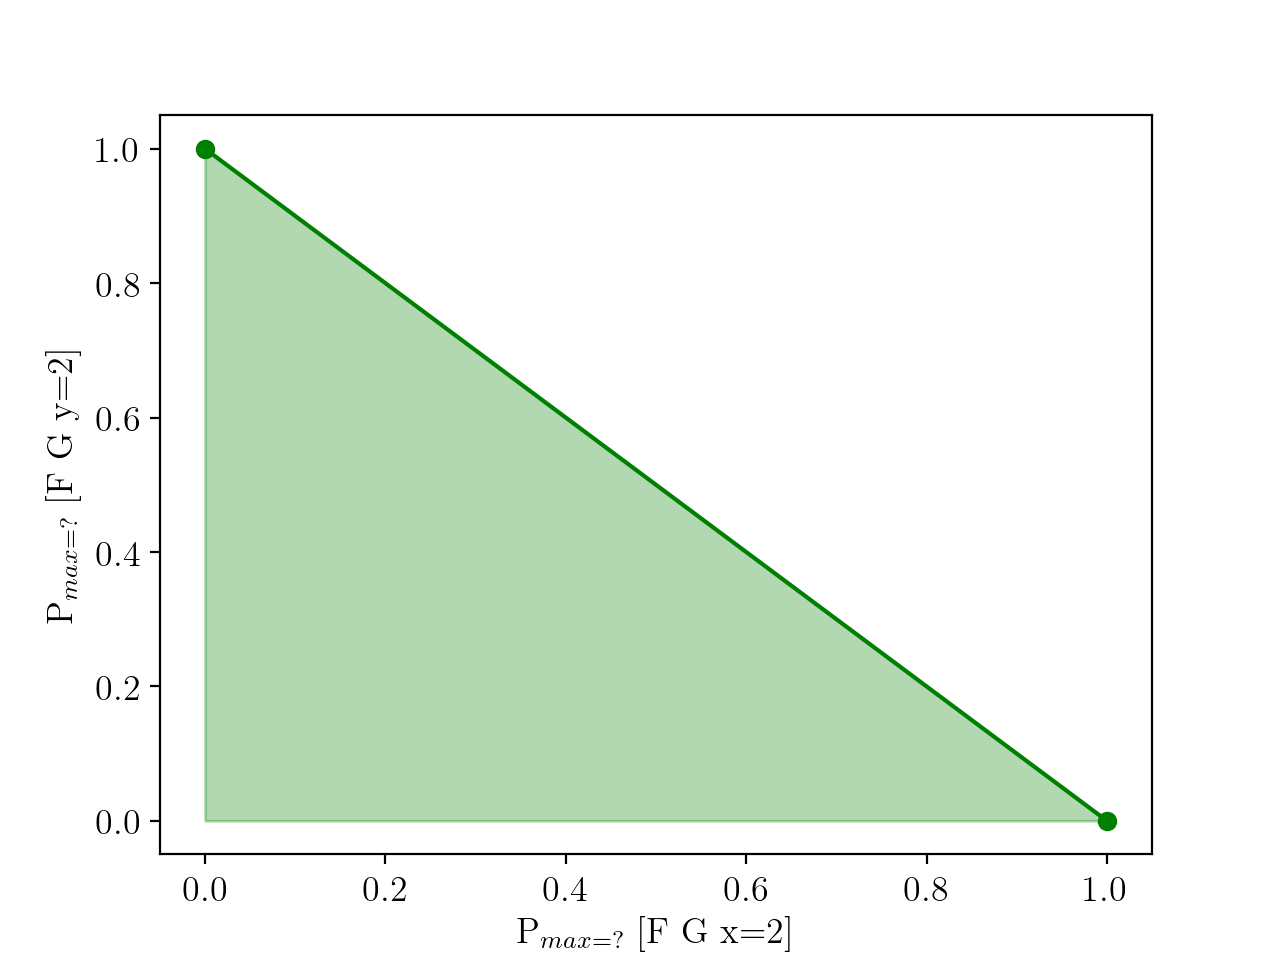
\includegraphics[width=0.9\textwidth]{pareto_1.png}
    \caption{Example of a Pareto curve represented as a 2D plot.}
    \label{fig:pareto_1}
\end{figure}

Each of the values resulting of the verification of quantitative properties in MDPs (whether they be a single value from a single optimisation, or a Pareto vector) is the result of an adversary which solves the nondeterminism and converts the MDP into a DTMC \cite{bk08}. The process of obtaining the adversary which satisfies certain properties is denoted by \textbf{strategy synthesis} or \textbf{adversary generation}, and it is formally defined below.

{\begin{defi}
{\setlength{\parskip}{2em}
\textbf{Strategy Synthesis (alternatively Adversary Generation)}\vspace{1em}\\}
{\setlength{\parskip}{1em} 

Consider a Markov decision process $\mathcal{M} = (S, Act, \mathbf{P}, p_{init}, AP, L)$. The process of maximal (similarly minimal) \textit{strategy synthesis} of the path formula $\varphi$ is defined as a process that yields an adversary $\sigma \in Adv$ such that:

\begin{equation}
	\sigma \in {\arg\sup}_{\sigma' \in Adv} P^{\sigma'}_s (\varphi)
\end{equation}

(respectively $\arg\inf$ for minimal), where $Adv$ is the set of all adversaries that $\mathcal{M}$ admits.

}
\end{defi}}


\chapter{Human Driver Modelling}
\label{sec:human_driver}

In this chapter, the human driver model that Salvucci presents in \cite{salvucci_1} is implemented and the metrics used to verify the model are established. Initially, the model is implemented in \textit{Matlab} based on the integrated driver model. To be able to verify it using the probabilistic model checking techniques presented in Chapter 2, the model undergoes an abstraction process, out of which a discrete-time Markov chain is obtained using several different approaches and assumptions. Metrics are then established to be able to evaluate whether the model meets the requirements and how well the human performs in a given situation. Finally, a simulator is presented in Section~\ref{sec:simulator} in order to allow visualisation of paths in the model.

\section{Continuous Driver Model using ACT-R}

In order to obtain a continuous driver model, we interpret Salvucci's integrated driver model as presented in \cite{salvucci_1}. The scenario considered is the one Salvucci envisioned: a multilane highway with moderate (or low) traffic \cite{salvucci_1}. The model uses the three modules presented in Figure~\ref{fig:high_level_salvucci}, that is, monitoring, decision making and control. All these modules rely on the constant update of the environment, as some are based on visual or low-level perception cues. While the human model is presented clearly in \cite{salvucci_1}, the dynamics of the car (which is part of the environment) are left to the reader, as it is outside the scope of the paper. In that sense, some assumptions had to be made about the environment.

The main initial assumption is that the driver is perfectly aware of its surroundings, and thus it is able to obtain the positions of other vehicles (within a certain distance) and the near and far points perfectly (this assumption is challenged later in the abstraction process). Additionally, the environment is assumed to change at the same rate as a cycle of the ACT-R model.

The overall view of the system is presented in Figure~\ref{fig:driver_model_overview}. The information flow is marked using the dotted arrows, while the sequential flow of the program is marked in the filled, lighter gray ones. Both the monitoring and the decision making make use of the perception which corresponds to querying the environment for the information (e.g. near and far point or another vehicle's position). The control both queries and sends updated information (e.g. vehicle position, velocity and acceleration) to the environment. Modules are updated sequentially, following the order: control, monitoring, decision making and environment (e.g. position, velocity and acceleration of other vehicles).

\vspace{1em}
\begin{figure}[h]
    \centering
    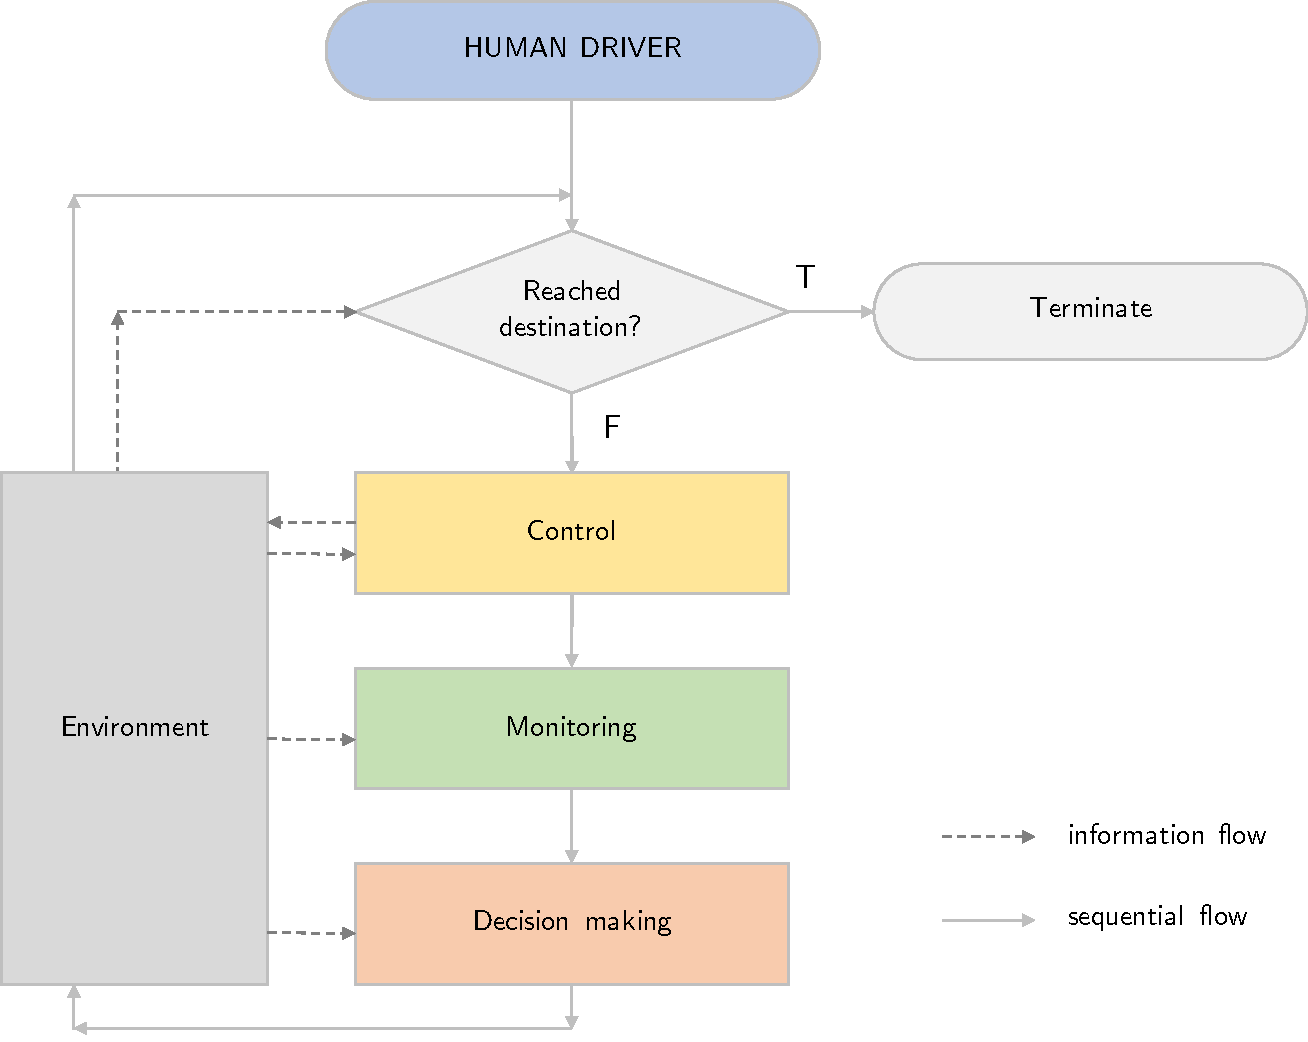
\includegraphics[width=0.85\textwidth]{matlab.pdf}
    \caption{Continuous Driver Model overview.}
    \label{fig:driver_model_overview}
\end{figure}

The monitoring module is implemented according to the flowchart presented in Figure~\ref{fig:monitor}, from the description given in \cite{salvucci_1}. The threshold for monitoring is set at $0.2$, as this is the value suggested by Salvucci in \cite{salvucci_1}. The output of this process corresponds to altering the global variable $a$ corresponding to the declarative memory cell composed of $k$ chunks. No specific value for $k$ is given by Salvucci in \cite{salvucci_1}, but it is taken to be 8 from \cite{lam}. The function \texttt{GET\_DISTANCE} is not described in depth due to the fact that it is trivial under the assumption stated previously.

The overall flowchart of the decision making module is shown in Figure~\ref{fig:dm}. The high level part is similar to the flowchart presented in Figure~\ref{fig:flowchart_dm}, with small differences related to the loading of variables and information from the different memories available. It is worth noticing that the control makes use of the function \texttt{LOOK\_VEHICLE} initially presented in the monitoring module to verify the presence of a vehicle in a relative position of a lane. The flow of the function \texttt{SET\_LANE\_FOLLOWING} is also omitted due to the trivial nature of this function under the assumptions made.

Finally, a flowchart for the control module is presented in Figure~\ref{fig:control}. This module is responsible for the calculation of $\Delta\varphi(t)$ and $\Delta\psi(t)$ and the update of the position. Given these two values, the position is updated following discrete laws of motion applied to rigid objects, particularly:

\begin{equation}
\begin{aligned}
	& \mathbf{v}(t) = \mathbf{v}(t-1) + \mathbf{a}(t)\Delta t\\
	& \mathbf{x}(t) = \mathbf{x}(t-1) + \mathbf{v}(t-1)\Delta t + \frac{1}{2}  \mathbf{a}(t)\Delta t^2 \\
	& t = t + \Delta t
\end{aligned}
\end{equation}

where $\mathbf{x}(t) = (x(t), y(t))$, $\mathbf{v}(t) = (v_x(t), v_y(t))$, and $\mathbf{a}(t) = (a_x(t), a_y(t))$, with:

\begin{equation}
\begin{aligned}
	a_x(t) & = \Delta\psi(t) \\
	a_y(t) & = \sin(\Delta\varphi(t))
\end{aligned}
\end{equation}

\begin{figure}
\centering
\begin{subfigure}{1\textwidth}
  \centering
  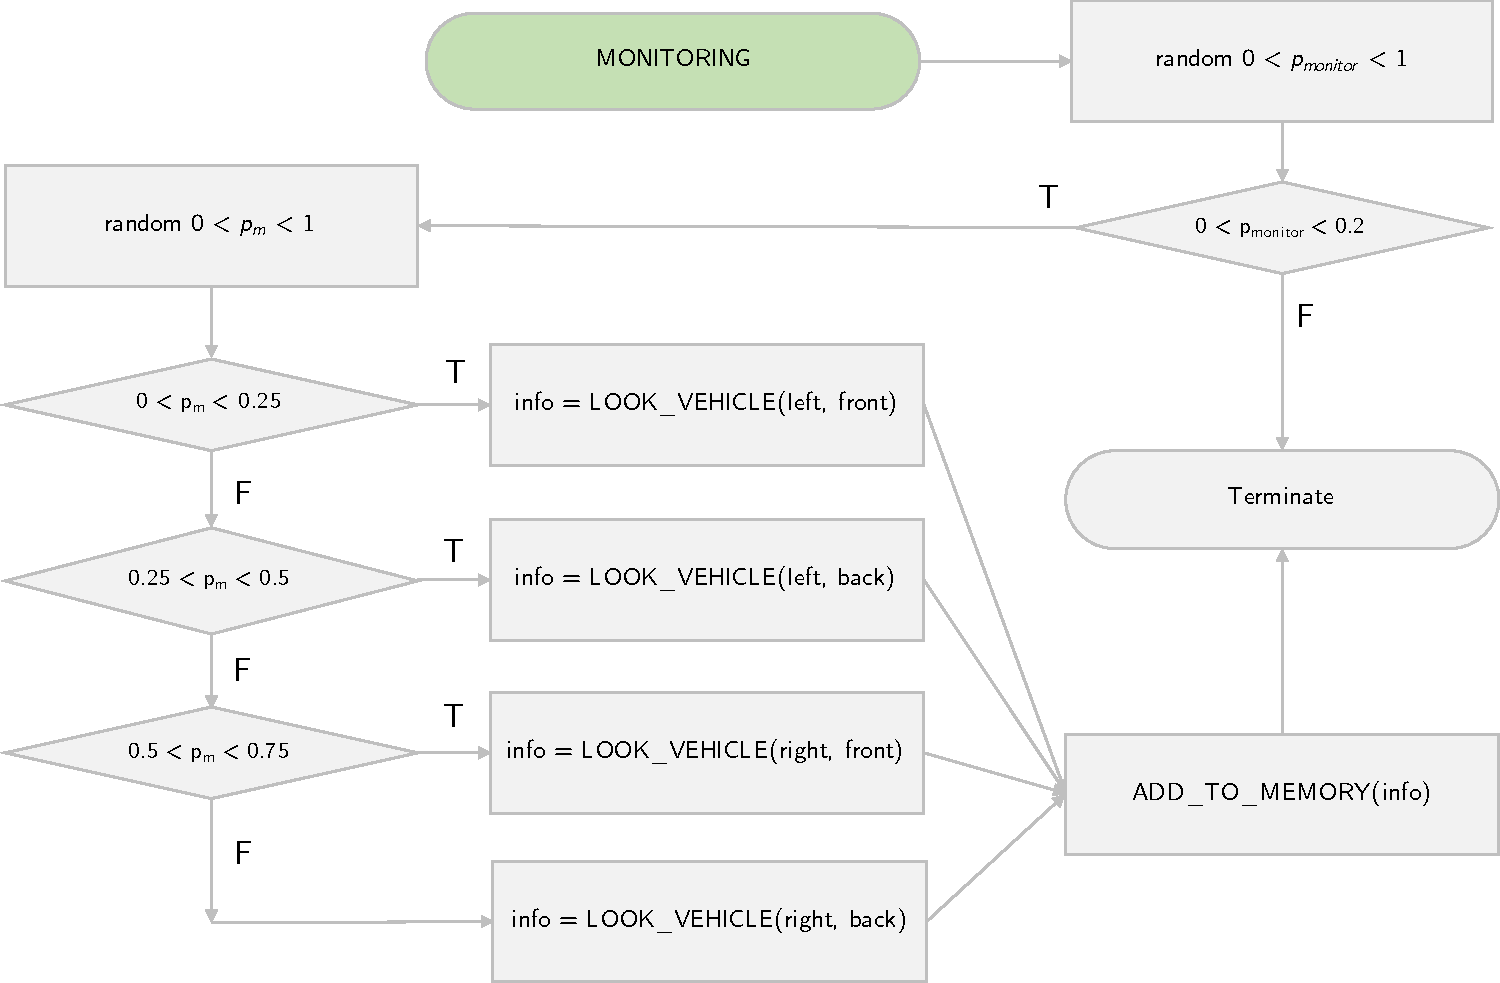
\includegraphics[width=1\textwidth]{monitor_1.pdf}
\end{subfigure}\\ \vspace{2em}
\begin{subfigure}{1\textwidth}
  \centering
  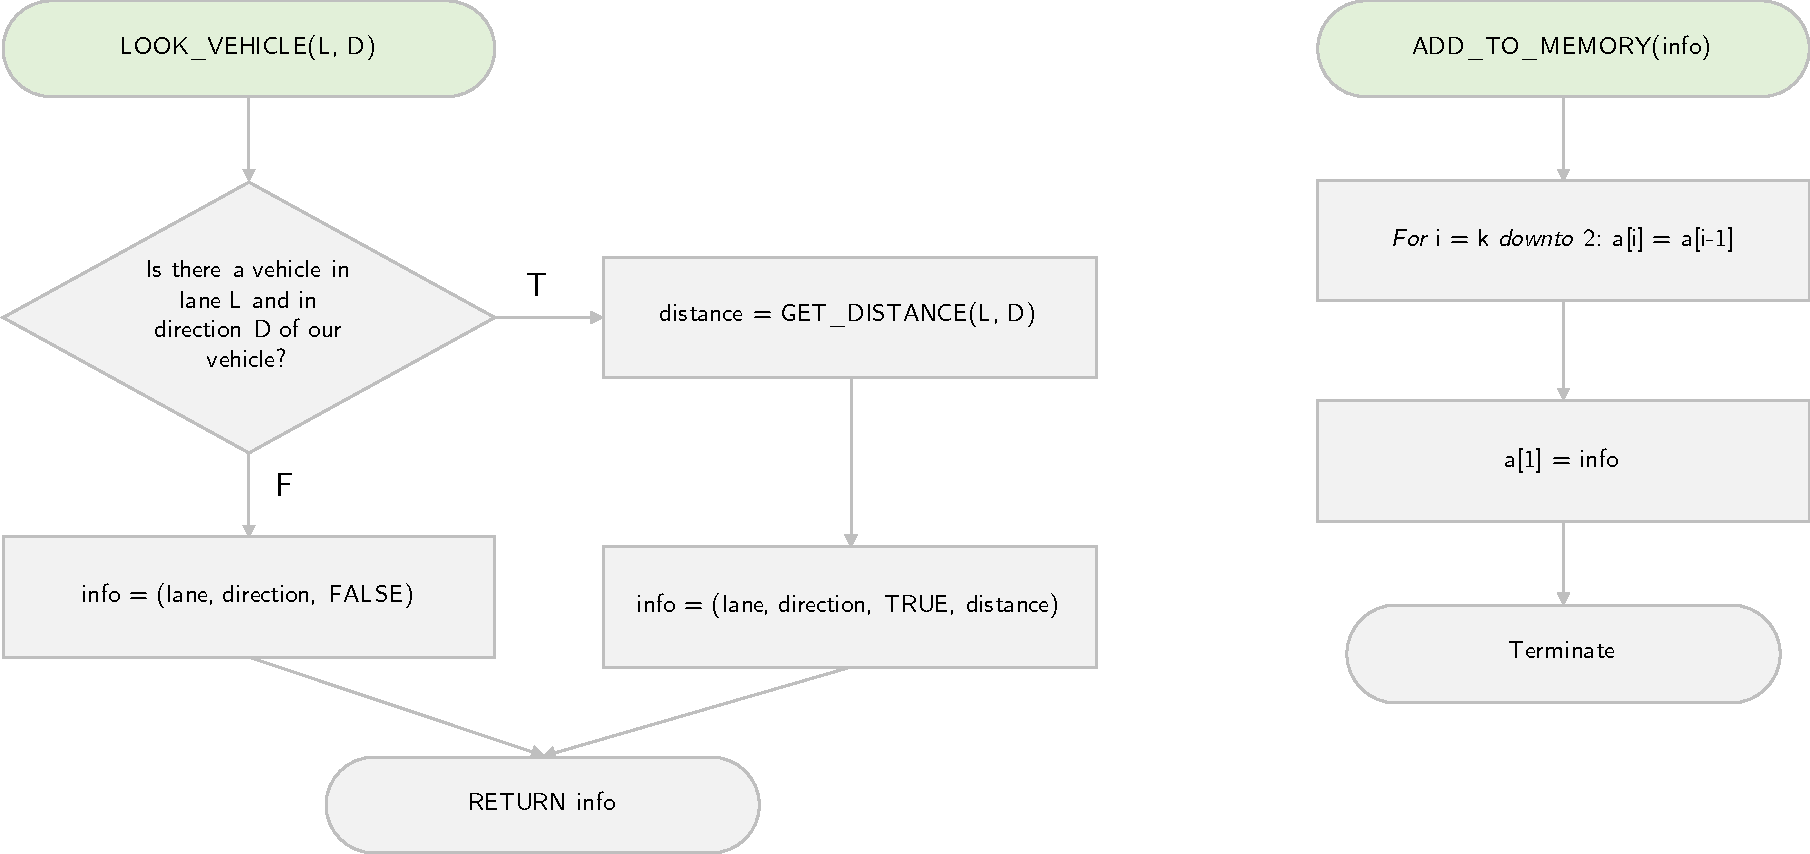
\includegraphics[width=1\linewidth]{monitor_2.pdf}
\end{subfigure} \vspace{2em}
\caption{Flowchart of the Monitoring module.}
\label{fig:monitor}
\end{figure}

\begin{figure}
\centering
\begin{subfigure}{1\textwidth}
  \centering
  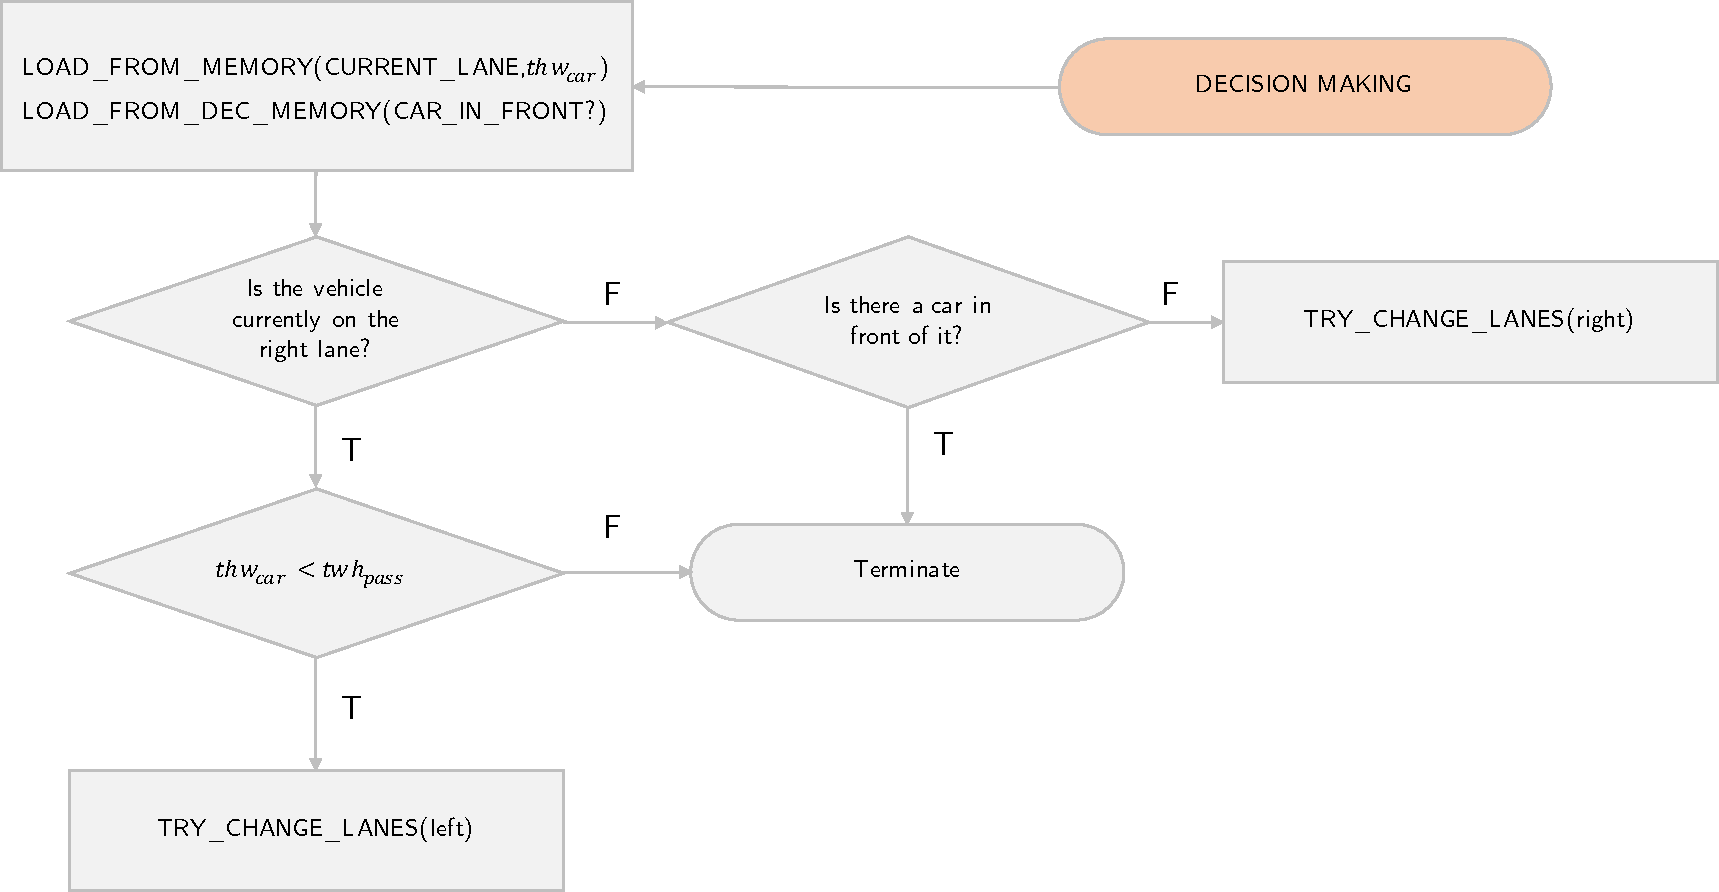
\includegraphics[width=1\textwidth]{dm_1.pdf}
\end{subfigure}\\ \vspace{2em}
\begin{subfigure}{1\textwidth}
  \centering
  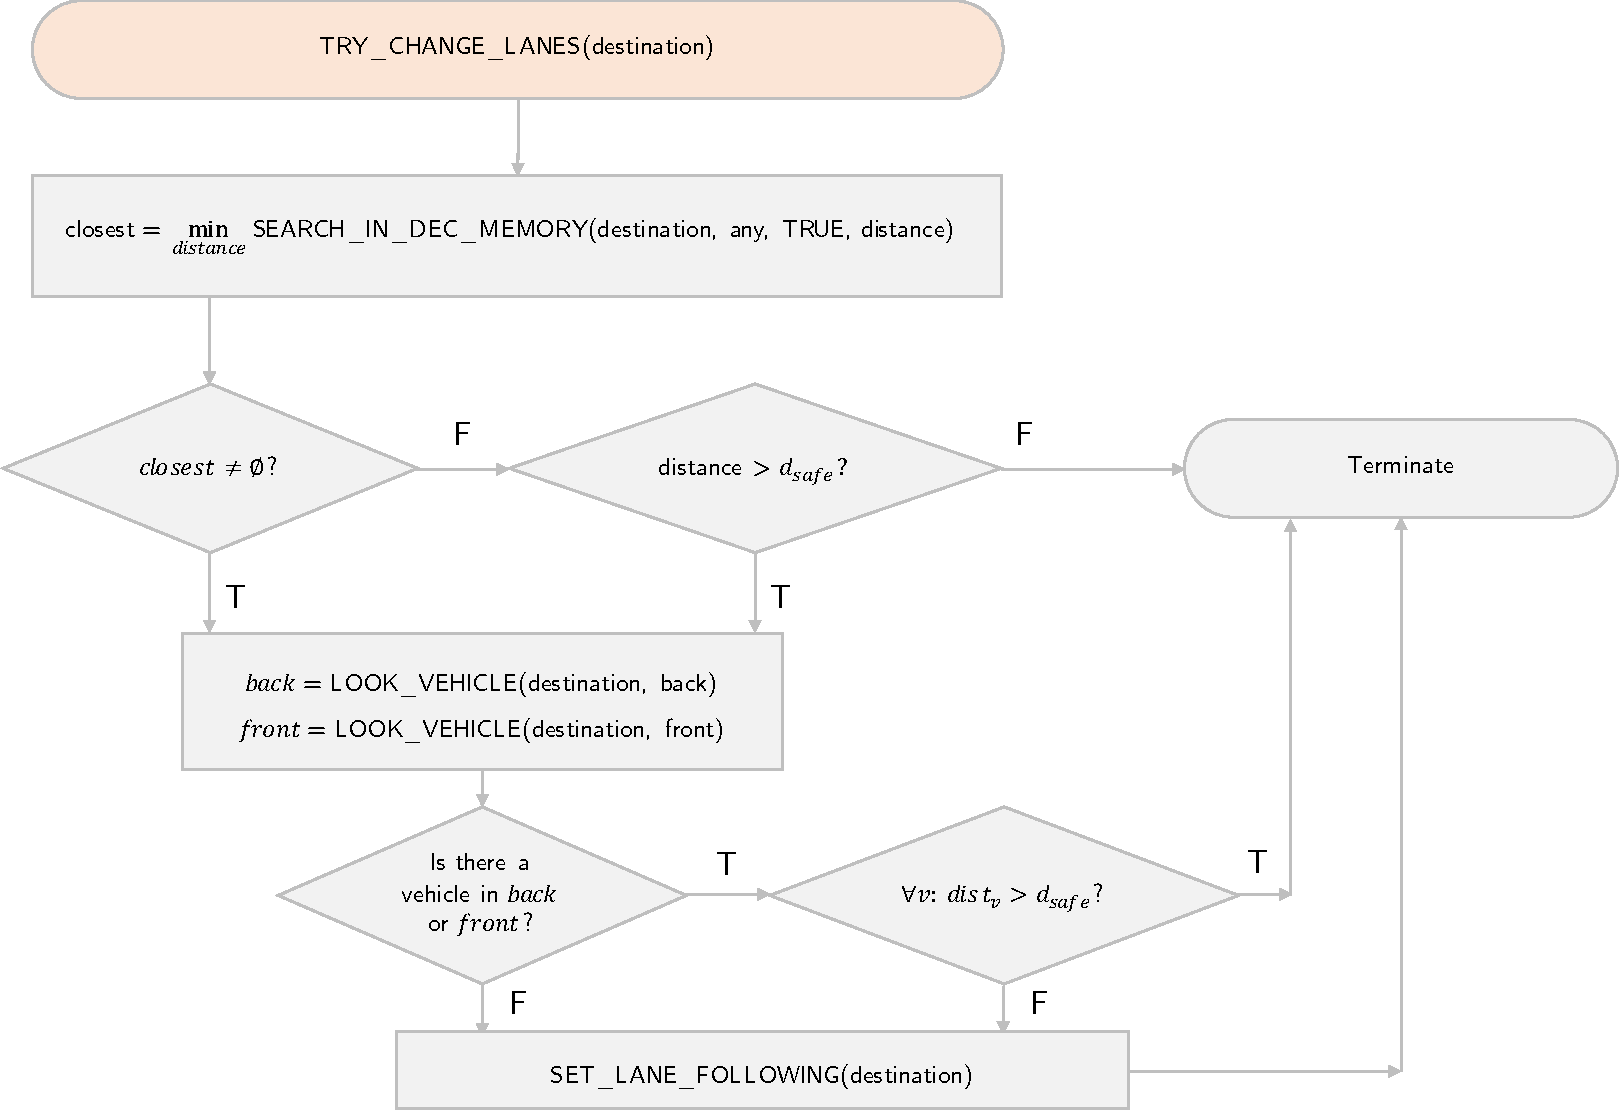
\includegraphics[width=1\linewidth]{dm_2.pdf}
\end{subfigure} \vspace{2em}
\caption{Flowchart of the Decision Making module.}
\label{fig:dm}
\end{figure}

\begin{figure}
\centering
\begin{subfigure}{1\textwidth}
  \centering
  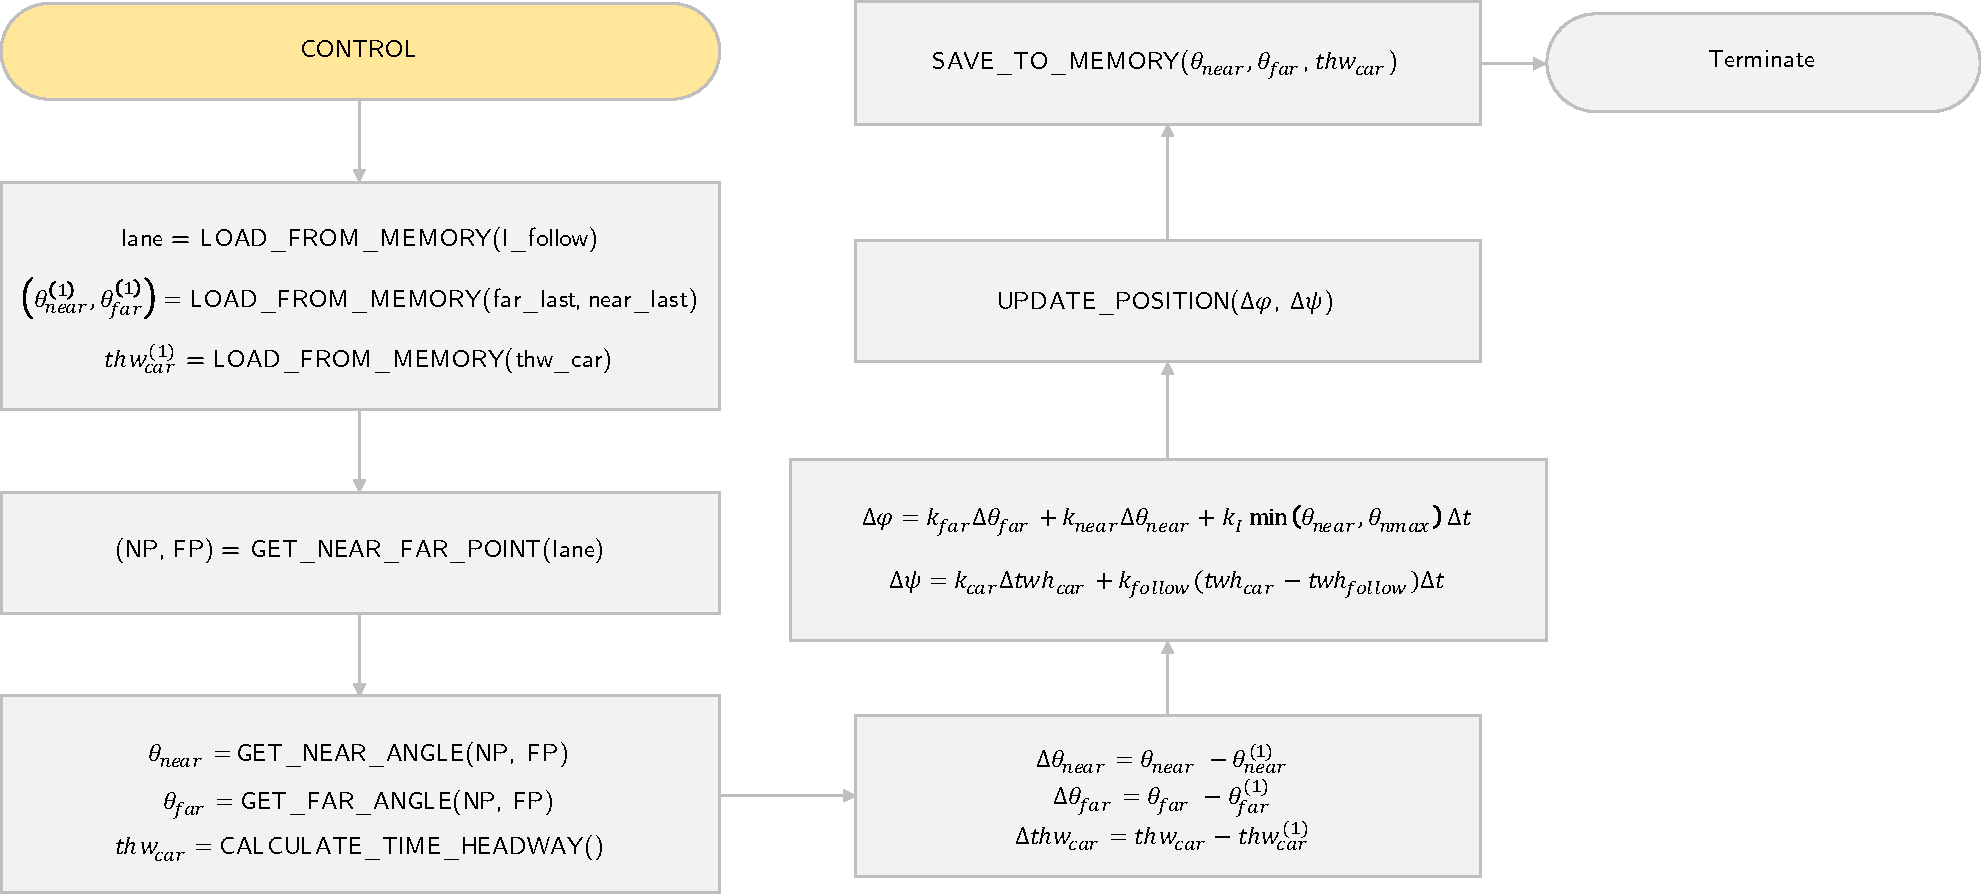
\includegraphics[width=1\textwidth]{control_1.pdf}
\end{subfigure}\\ \vspace{2em}
\begin{subfigure}{1\textwidth}
  \centering
  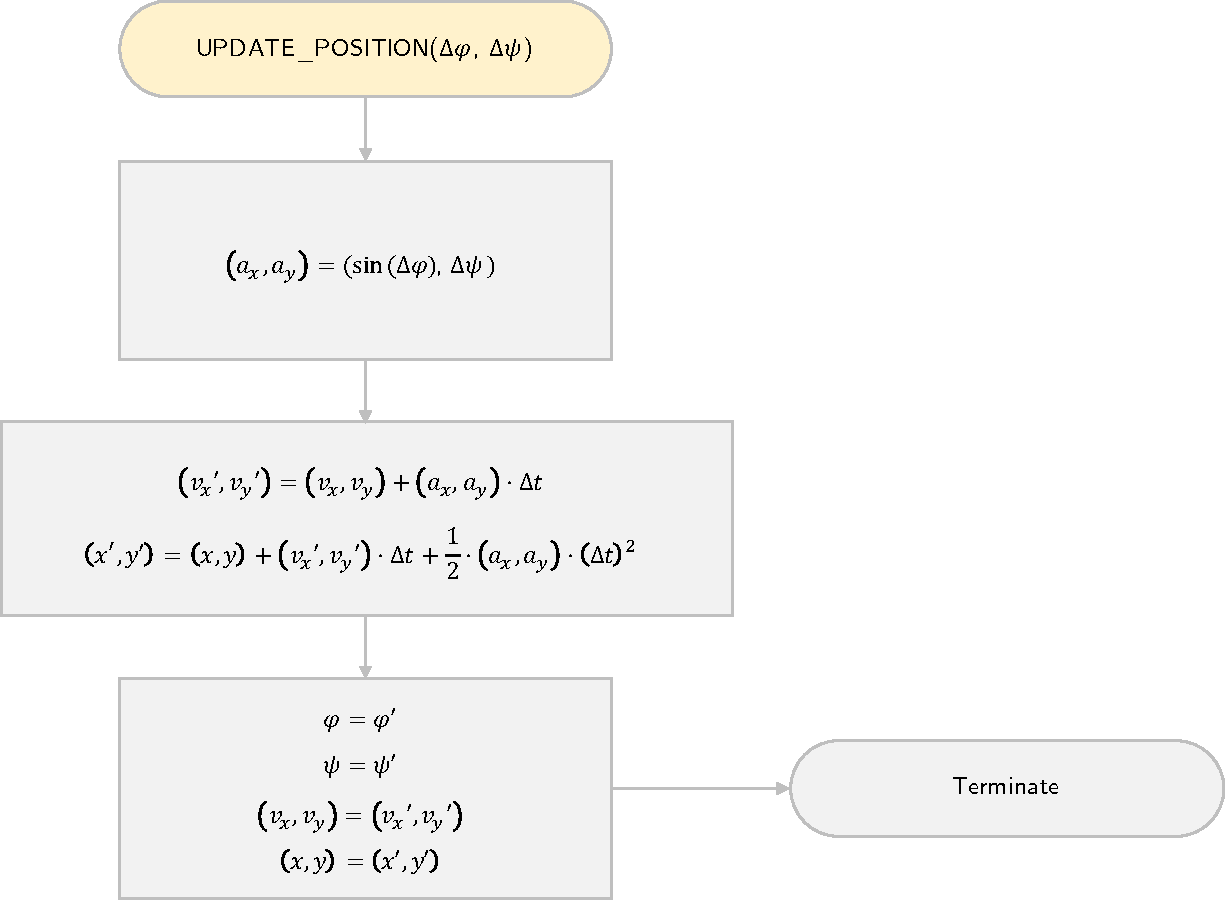
\includegraphics[width=0.7\linewidth]{control_2.pdf}
\end{subfigure} \vspace{2em}
\caption{Flowchart of the Control module.}
\label{fig:control}
\end{figure}

In this case, as Salvucci mentions in \cite{salvucci_1}, $\Delta t = 0.5s$. It is also assumed that the vehicle complies with the speed limits, and, therefore, $v_x \in [15, 34]\text{ }m/s$ (between $50km/h$ and $120km/h$ - typical limits in highway speeds).

Using these assumptions, the continuous driver model is implemented in \textit{Matlab} as presented in Appendix~\ref{sec:appendix_cont}.

\section{Model Abstraction}

The process of abstraction consists in transforming the evolution of the continuous variables that constitute the model and discretising it in order to obtain a finite discrete model. In this case, the goal is to go from the continuous model of driver behaviour presented in the previous section to a discrete-time Markov chain (DTMC) which represents the same process. This transformation is less than trivial due to the fact that, in model checking of finite state abstractions, as the number of state variables in the system increases, the size of the system state space grows exponentially \cite{state_explosion}. This problem is known as state explosion, and there has been some research into efficient ways of dealing with it \cite{abstraction_1, abstraction_2}. 

In the following sections, the abstraction process for the different modules of ACT-R is presented in detail, as well as the thought process behind the choices made. Finally, the unified model is presented using the different modules designed.

\subsection{Non-Probabilistic Control Module}
\label{sec:non_prob_control}

The control module, as presented in the previous section and following Salvucci's approach in \cite{salvucci_1}, is fully deterministic, in the sense that there is no probabilistic reasoning involved. It makes use of perception (for the near and far points) and two simple control laws which influence the position, velocity and acceleration of the vehicle in the environment.

The straightforward approach to this problem would be to represent it as a simple $N\times M$ grid, in which a tuple $(x,y)$ with $x\in \{0,...,N\}$ and $y\in \{0,...,M\}$ would describe the position of the vehicle, and all other variables (i.e. $v_x$, $v_y$, $a_x$, $a_y$ and $t$) would be integer versions of its continuous model representation. In this approach, the control laws could be applied directly over the grid and the results would be the movement of the vehicle in it. However, there is an intrinsic problem with this approach. The error associated with the use of the grid as a way to discretise space would, logically, be reduced with an increase of $N$ and $M$ for a representation of the same road segment (i.e. increase in resolution). For example, the error associated with a road segment of $500 \times 7m^2$ represented by $N = 500$ and $M = 7$ (each grid square corresponds to $1m^2$) would be significantly greater than if $N = 5000$ and $M = 70$ (each grid square corresponds to  $10^{-2}\text{ }m^2$). The conclusion would be that one should increase $N$ and $M$ in order to obtain an appropriate resolution, but this incurs in the problem of state explosion presented in the beginning of the section: as the variable ranges increase, the number of states in the system grows exponentially. Thus, while the situation of $N = 5000$ and $M = 70$ is appealing in terms of error minimisation, it would be intractable to actually build and perform model checking on it (e.g. for $v_x, v_y \in \{15,...,34\}$ and $a_x, a_y \in \{-3,...,3\}$, the control module alone would have approximately $6.89\times 10^{9}$ states, making it impossible to add decision making and monitoring on top of it). 

The straightforward strategy is not, by any standards, efficient in terms of state space and does not use any of the information of the problem to simplify it. In particular, one should notice that, in this scenario, the movement in the $y$ direction is used simply for the purpose of lane changing, a process which is purely deterministic (as described in \cite{salvucci_1}). Therefore, a more interesting approach to the abstraction of the control module could take this into account and \textbf{pre-simulate the lane changing operations}.

In this approach, the vehicle's position is represented by two discrete integer variables $x \in \{0,...,length\}$ for a given $length$ and $lane \in \{right, left\}$ (can be extended to more than two lanes), and the acceleration and velocity of the vehicle are simply $a = a_x$ and $v = v_x$. Time is still represented in the same way, with $t \in \{0,...,max\_time\}$. If a lane change is decided by the decision making module, then, \textbf{within one transition of the control}, the $lane$ variable is updated with the final destination lane, and the variables $x, v, a$ and $t$ are updated to reflect the obtained values after a lane change. These values are obtained from a look-up table and depend on the distance to the other vehicle ($d$) and the velocities of both the vehicle in question ($v$) and the other vehicle ($v_1$) (an obstacle on the road can be modelled by setting $v_1 = 0$). Additionally, the variable $crashed$ is used to represent whether the vehicle has collided in the process or not. The linear acceleration is implemented similarly using pre-simulation to determine the value of acceleration and the motion law is updated in the model itself.

The continuous model of driver behaviour obtained in the previous section in \textit{Matlab} is used as the basis for the simulation of lane changes and linear acceleration. From this model, look-up tables are obtained which, given an origin lane ($o_{lane}$), a distance to the other vehicle and the velocities of both the vehicle in question and the other vehicle determines whether a crash happened or not, what is the $\Delta x$ and $\Delta T$ incurred (how did the position in $x$ changed and how long did it take), and the final velocity of the vehicle in question. The code presented in Appendix~\ref{sec:control_abs} corresponds to a similar version of the control (but probabilistic, as presented later in this section). An example of the simulation of the scenario $o_{lane} = 1$, $d = 20m$, $v = 15m/s$ and $v_1 = 15m/s$ is shown in Figure~\ref{fig:lane_change_ex}.

\begin{figure}[h]
    \centering
    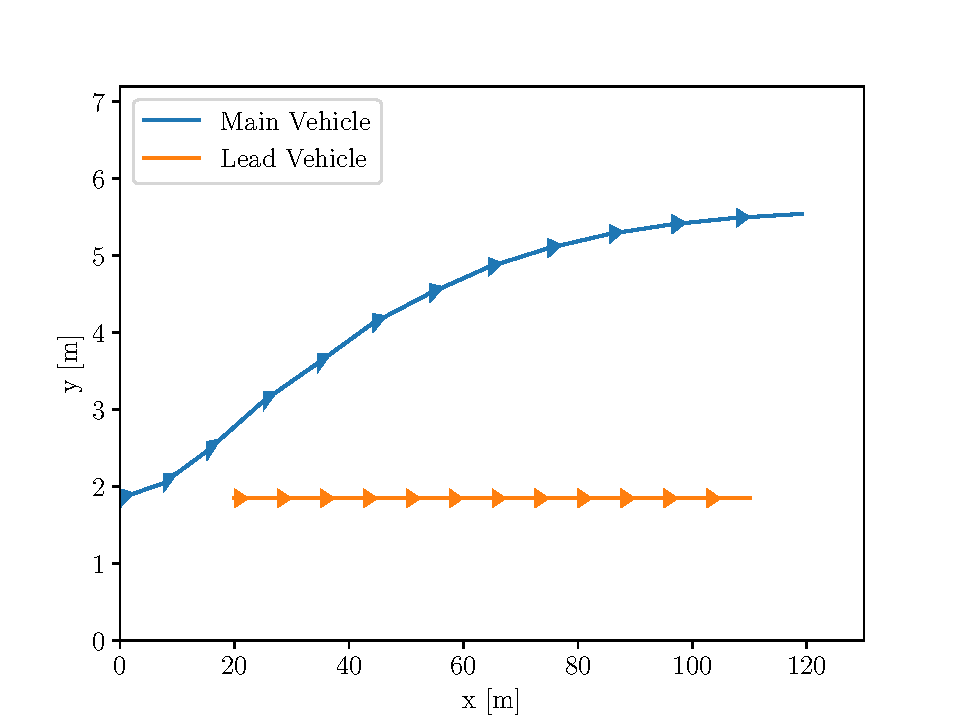
\includegraphics[width=0.9\textwidth]{lane_change_ex.pdf}
    \caption{Example of the simulation of the lane change for $o_{lane} = 1$ (right lane), $d = 20m$, $v = 15m/s$ and $v_1 = 15m/s$. In this case, after the change is complete the variable assignments are $crashed = 0$ (no collision happened), $\Delta x = 119m$, $\Delta T = 6s$ and $v = 23m/s$.}
    \label{fig:lane_change_ex}
\end{figure}

This process focuses the computational effort on the pre-calculations, simplifying the final model significantly in terms of the state space, while removing the error made by discretising in the $y$ direction of the grid (the error in the $x$ direction is still present though). With regards to the size of the lane changing table, for the considered scenario of $2$ lanes, $v, v_1 \in \{15,...,34\}$ and for any discrete $d \in \{1,...,length\}$, the size of the table would be $2\times 20^2 \times length = 800 \times length$. Given that the only value of the table that is effectively altered with a change in $d$ is the value of $crashed$ (as the $\Delta x$, $\Delta T$ and final $v$ depend solely on the initial velocities of both vehicles), it is possible to define $d_{\max}$ such that:

\begin{equation}
d_{\max} < length\text{, s.t. }\forall v, v_1 \in \{15,...,34\}, d' \geq d_{\max}: crashed_{d'} = false
\end{equation}

that is, $d_{\max}$ is a great enough value of $d$ such that, regardless of the speed of the two vehicles, no crash will occur between them. With this change, it is possible to reduce the table from $800\times length$ to $800\times d_{\max}$ (since all other rows would be equal to the one for $d_{max}$). For the given ranges of $v$ and $v_1$, $d_{\max}$ is determined to be $43m$, and thus the obtained look-up table contains $34,400$ rows.

The linear acceleration table depends on the $thw_{car}$ which varies only with the distance to the other vehicle and the current velocity of the vehicle in question. Considering the distance in this case to be up to $80m$ (otherwise maximum acceleration will be applied), the look-up table generated has $1,600$ rows.

\subsection{Decision Making and Monitoring Module}

Due to the fact that, in the model presented by Salvucci in \cite{salvucci_1}, the monitoring module influences the declarative memory which is then used exclusively for decision making purposes (and not for control), logically these two can be incorporated into one for abstraction purposes. Again, taking the straightforward approach of trying to include the declarative memory and the process associated with monitoring and decision making into the model directly would make it intractable. 

In its simplest form, the decision making process for the right lane consists in localising the other vehicle and deciding whether or not to change lanes based on the time headway, $thw_{car}$, to the lead vehicle (if there is one). This value essentially corresponds to the time the vehicle in question has before it crashes into the lead vehicle, assuming that latter came to a full stop ($v = a = 0$) \cite{thw}. The lower this time headway, the more likely a driver is to perform the manoeuvre. While Salvucci presents a fully deterministic driver in \cite{salvucci_1} based on the average driver, in this dissertation it was decided to try and analyse drivers according to different profiles in order to simulate how different parts of the population of drivers might make decisions. The decision making in such a case follows from a stochastic reasoning which can be simulated and incorporated in the model using look-up tables. 

In this case, for a driver in the right lane, it was decided to model the probability of the driver performing a lane change based on the time headway as an exponentially decreasing function, writing it as:

\begin{equation}
	\text{P[}lC = true\text{]}_{thw} = P_{lC}(d,v) = e^{-\alpha\cdot thw} = e^{-\alpha\cdot d/v}
\end{equation}

where $\alpha$ is a parameter unique to each population of drivers. 

The same logic can be applied for a driver in the left lane overtaking a vehicle behind it in the left lane, except in this case the opposite effect will be seen in the decision making. In such a case, the probability of changing lane can be modelled as a normalised logarithmic function over the distance of the vehicles (it doesn't make sense to define time headway in this context):

\begin{equation}
	\text{P[}lC = true\text{]}_{d} = P_{lC}(d) = \frac{1}{\log(\beta\cdot \max_d + 1)}\cdot \log(\beta\cdot d + 1)
\end{equation}

where $\max_d$ is the maximum length considered and $\beta$ is a parameter unique to each population of drivers.

It should be noted that these functions, while logical, are an assumption of the abstraction, since the model presented by Salvucci in \cite{salvucci_1} does not make any reference to these parameterisations. It is also worth referring that, while there was no real-world data involved in this project, this function could have been learnt from real data without changing the fundamental paradigm of the abstraction.

For the purposes of analysis, three classes of drivers are considered: \textbf{Aggressive}, \textbf{Average} and \textbf{Cautious} drivers (with different values for the parameter $\alpha$ and $\beta$). In Figure~\ref{fig:dm_curves}, the functions are presented for the three profiles of drivers assumed in this project, for the lane changes originating in the right (Figure~\ref{fig:dm_curve_right}) and left lane (Figure~\ref{fig:dm_curve_left}).

\begin{figure}
\centering
\begin{subfigure}{1\textwidth}
	\centering
	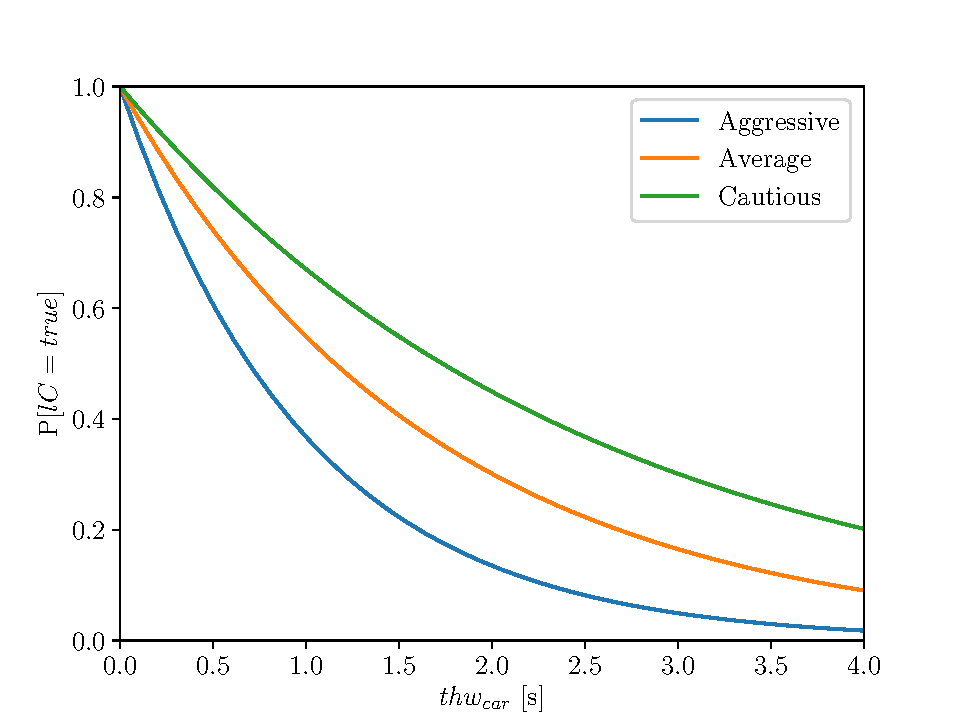
\includegraphics[width=0.85\textwidth]{dm_curve.pdf}
	\subcaption{Aggressive ($\alpha = 1$), Average ($\alpha = 0.6$) and Cautious ($\alpha = 0.4$) drivers.}
	\label{fig:dm_curve_right}
\end{subfigure}\\
\begin{subfigure}{1\textwidth}
	\centering
	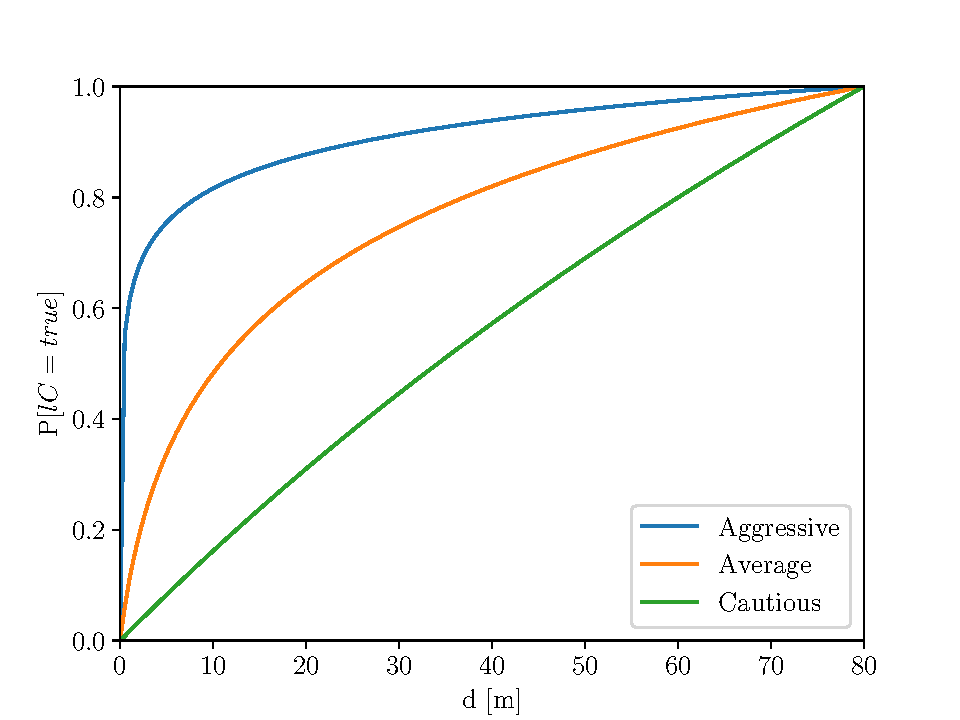
\includegraphics[width=0.85\textwidth]{dm_curve_2.pdf}
	\subcaption{Aggressive ($\beta = 1000$), Average ($\beta = 0.5$) and Cautious ($\beta = 0.01$) drivers.}
	\label{fig:dm_curve_left}
\end{subfigure}\vspace{1em}
\caption{$\text{P[}lC = true\text{]}$ as a function of $thw_{car}$ and $d$ for vehicles originating from the right lane (a) and left lane (b).}
\label{fig:dm_curves}
\end{figure}

So far, this version of decision making is not influenced by the monitoring module at all, and it relies on the correct calculation of the value of $thw_{car}$ and $d$. This assumption is unrealistic, and in order to simulate these issues, it was decided that stochastic noise could be added to the measurement of the distance (as this is what human drivers have to instinctively measure through perception). It was chosen that this noise, $n$, would be normally distributed as:

\begin{equation}
	n \sim \mathcal{N}(0, \sigma)
\end{equation}

such that:

\begin{equation}
	thw'_{car} = thw_{car} + n(thw_{car})
\end{equation}

Alternatively, this can be represented directly as (using discrete integration steps of width $\delta$):

\begin{equation}
\begin{aligned}
	P'_{lC}(d,v) & = \sum_{i = -\infty}^{+\infty} [N(d + i + \delta/2) - N(d + i - \delta/2)] \cdot P_{lC}(d + i,v) \\
	& = \sum_{i = -\max_d}^{+\max_d} [N(d + i + \delta/2) - N(d + i - \delta/2)] \cdot P_{lC}(d + i,v)
\end{aligned}
\end{equation}

where $\max_d$ is the maximum length considered and $N(d)$ corresponds to the cumulative probability function (CDF) defined as:

\begin{equation}
	N(d) = \int_{-\infty}^d n(t) dt
\end{equation}

From this, a look-up table can be generated which, for different driver types, yields the probability of lane changing for a certain distance to the lead car and velocity. For the 3 driver profiles mentioned, considering $d \in \{1,...,80\}$ ($\max_d = 80$) and $v \in \{15,...,34\}$, the table generated for the vehicle in the right lane has $4,800$ rows \footnote{In the data obtained for the results presented in this dissertation, $\delta = 1$.}. Under the same conditions, the look-up table for the vehicle in the left obtained has $240$ rows (the difference is explained by the fact that the velocity does not influence this table). Thus, the unified decision making table has $5,040$ rows.

The code presented in Appendix~\ref{sec:dm_abs} corresponds to the methods used to obtain the unified look-up table used for the decision making and monitoring module.

\subsection{Probabilistic Control Module}
\label{sec:prob_control}

In light of the uncertainty introduced in the decision making and monitoring module regarding the visual perception of distance, it becomes only natural that this would be extended to the control module as well. In order to cope with this, a probabilistic version of the control module was designed, where the noise $n$ presented in the previous section is taken into consideration. 

In order to obtain the equivalent look-up tables for the probabilisitic control module, the \textbf{Monte Carlo method} can be used. In this case, the noise can be simulated in repeated trials, and an average can be obtained for the crashing probability, the estimated final difference in position, the estimated difference in time and estimated final velocity of the vehicle. In the case of this dissertation, the tables generated (for linear and lane changing control) were the result of 100 trials.

The code presented in Appendix~\ref{sec:control_abs} corresponds to the simulation of this probabilistic version of the control, which generates the linear and steering control tables.

\subsection{Unified Two-Module Model}

Using the three tables generated (two for the probabilisitic control - linear and steering control - and one for the decision making), the final DTMC model unifies both using a sequential variable $actr\_state \in \{1,2\}$, where $actr\_state = 1$ corresponds to the control and $actr\_state = 2$ corresponds to decision making. In the version of the unified model built for this thesis, only two vehicles are present: the first is the one controlled by the driver and the second is a lead vehicle starting at a distance $x = x_{1,0}$ (in meters) from the main vehicle (which starts at $x=0$) and moves with a constant speed of $v_1$ on a road segment of $length$ meters. The movement of the lead vehicle is, therefore, completely determined by the formula:

\begin{equation}
	x_1(t) = x_{1,0} + v_1\cdot t
\end{equation}

The distance between the two vehicles can be obtained as:

\begin{equation}
	d(t) = \lvert x(t) - x_1(t) \rvert
\end{equation}

And the boolean function $posDist$ can be defined as:

\begin{equation}
posDist(t) = 
     \begin{cases}
       \text{true,} &\quad\text{if }x(t) \geq x_1(t)\\
       \text{false,} &\quad\text{otherwise.} \\
     \end{cases}
\end{equation}

Due to the large size of the tables generated, the models should be generated automatically for a given tuple of initial conditions $(d_{type}, v, v_1, x_{1,0})$ (where $d_{type}$ is the driver class according to the ones defined in the decision making and monitoring subsection - 1 is aggressive, 2 is average and 3 is cautious), following the assumptions described below:

\textbf{General assumptions}

\begin{enumerate}
	\item A transition from state $s$ to state $s'$ is possible if, and only if, the variable $actr\_state$ takes different values in $s$ and $s'$.
	\item A transition from state $s$ to state $s'$ is possible if, and only if, $t_{s'} \geq t_s$ (where $t_{\alpha}$ is the value of variable $t$ in state $\alpha$).
	\item The model should have no states with self transitions, as there is always a continuous evolution of the state of the vehicles.
	\item A deadlock state should only be entered if, and only if, the vehicle either crashes ($crashed = true$) or reaches the end of the road ($x = length$).
\end{enumerate}

\textbf{Control ($actr\_state = 1$)}

\begin{enumerate}
	\item If no lane change has been decided, the model reasons over linear acceleration using the corresponding look-up table for $d(t)$ and $v(t)$, and updates the state variables $t, x, v, a$ and $crashed$ accordingly using the discrete laws of motion previously presented.
	\item If a lane change has been decided, the model reasons over the lane change using the corresponding look-up table for $o_{lane}$, $d(t)$, $v(t)$, $v_1$, and updates the variables $x$ and $t$ incrementally using the values $\Delta x$ and $\Delta T$ of the table, as well as sets the value of $v$ and $crashed$.
\end{enumerate}

\textbf{Decision Making and Monitoring ($actr\_state = 2$)}

\begin{enumerate}
	\item If the vehicle is on the left lane and behind the other vehicle ($lane=left$ and $posDist = false$), the model will not attempt a lane change.
	\item If the vehicle is on the left lane and in front of the other vehicle ($lane=left$ and $posDist = true$), the model will reason over lane changes using the decision making and monitoring look-up table for $d_{type}$.
	\item If the vehicle is on the right lane and behind the other vehicle ($lane=right$ and $posDist = false$), the model will reason over lane changes using the decision making and monitoring look-up table for $d_{type}$.
	\item If the vehicle is on the right lane and in front of the other vehicle ($lane=left$ and $posDist = true$), the model will not attempt a lane change.
\end{enumerate}

From these rules and the tables obtained in the abstraction of the individual modules, it is possible to build a model generator. The code for an example of such a generator written in \textit{Python} (used throughout the rest of the dissertation) is presented in Appendix~\ref{sec:two_module_gen}. 

By running the model generator using the conditions $(d_{type}, v, v_1, x_{1,0}) = (1,30,22,51)$, that is, an aggressive driver, starting at $30m/s$ with another vehicle going at $22m/s$ and starting at $51m$, the resulting model description is the one presented in Listing~\ref{lst:model_example} (shortened for the sake of space saving; the full model is $13,435$ lines long).

{\vspace{1em}
\begin{lstlisting}[caption={Example of the model generated for the tuple $(d_{type}, v, v_1, x_{1,0}) = (1,30,22,51)$ (shortened)},captionpos=b,label={lst:model_example}]
//Model automatically built using model_generator.py for v1 = 22 and driver_type = 1 (to alter these values, run the script again).
//Generated on 31-07-2018 at 18:47.

dtmc

const int length = 500; // road length
const int driver_type = 1; // 1 = aggressive, 2 = average, 3 = cautious drivers - do not alter this manually!
const int max_time = 35; // maximum time of experiment

// Other vehicle
const int v1 = 22; // do not alter this manually!
const int x1_0 = 51;

// Environment variables
global t : [0..max_time] init 0; // time 
global crashed : bool init false; 

// Vehicle controlled
global actrState : [1..2] init 1; // active module: 1 = control (both cars), 2 = decision making + monitoring
global lC : bool init false; // lane changing occuring? 
global x : [0..length] init 0;
global v : [15..34] init 30;
global a : [-2..3] init 0;
global lane : [1..2] init 1;

formula x1 = x1_0 + v1*t;
formula dist = x1>x?(x1 - x):(x - x1);
formula positiveDist = (x < length)?x > x1:true;

module Decision_Making_Monitoring

 	// If a crash occurs, then nothing else can happen
	//[] actrState = 2 & crashed -> 1:(crashed' = true);

 	// If we are in lane 2, but behind the other vehicle, don't try to pass
	[] actrState = 2 & !crashed & lane = 2 & positiveDist = false -> 1:(actrState' = 1);

	// If we are in lane 1, and no vehicle is in front, don't change lanes
	[] actrState = 2 & !crashed & lane = 1 & positiveDist = true -> 1:(actrState' = 1);

	[] actrState = 2 & !crashed & lane = 1 & positiveDist = false & dist = 1 & v = 15 -> 0.8:(actrState' = 1) & (lC' = true) + 0.2:(actrState' = 1) & (lC' = false);

	...

	[] actrState = 2 & !crashed & lane = 2 & positiveDist = true & dist >= 80 -> 1:(actrState' = 1) & (lC' = true) + 0:(actrState' = 1) & (lC' = false);
endmodule

module Control

 	// If we are in lane 1, and no lane change was decided, continue forward (which might result in crash)
 	// The vehicle is behind the other driver (positiveDist = false, x < x1)
	[] actrState = 1 & !crashed & !lC & lane = 1 & x <= length - v & t < max_time & positiveDist = false & (x1 + v1 - x - v) >= 6 & v + a < 34 & v + a > 15 & dist = 1 & v = 15  -> 1:(x' = x + v) & (t' = t + 1) & (v' = v + a) & (a' = -2) & (actrState' = 2);

	...

	[] actrState = 1 & !crashed & lC & lane = 2 & dist >= 43 & v = 34 & x > length - 136 & t > max_time - 6 -> 1:(crashed' = false) & (x' = length) & (v' = 34) & (t' = max_time) & (a' = 0) & (lane' = 1) & (actrState' = 2) & (lC' = false);

endmodule
\end{lstlisting}
}

By loading and building the model in either PRISM or Storm, it is observable that it has 257 states and 295 transitions, a significant reduction from the possibilities presented in the straightforward control abstraction. Due to the fact that there are $3\times 20 \times 20 \times length$ different possibilities in terms of initial conditions, it would be intractable, in the timeline of the dissertation, to obtain the number of states for all the combinations. Table~\ref{tab:sta_tra_example} presents the number of states and transitions for some arbitrarily generated conditions (for a road of length $500m$).

{
\vspace{1em}
\bgroup
\def\arraystretch{1.3}
\begin{table}[h]
\centering
\begin{tabular}{|c|c|c|c||c|c|}
\hline
\textbf{$d_{type}$} & \textbf{$v$} & \textbf{$v_1$} & \textbf{$x_{1,0}$} & \textbf{\# States} & \textbf{\# Transitions} \\ \hline \hline
3 & 21 & 30 & 20 & 305 & 333 \\ \hline
1 & 27 & 22 & 66 & 396 & 471 \\ \hline
1 & 28 & 17 & 43 & 167 & 183 \\ \hline
2 & 33 & 15 & 35 & 6 & 7 \\ \hline
3 & 28 & 21 & 38 & 199 & 222 \\ \hline
1 & 19 & 16 & 81 & 391 & 443 \\ \hline
2 & 25 & 23 & 28 & 390 & 481 \\ \hline
3 & 15 & 17 & 36 & 487 & 569 \\ \hline
1 & 29 & 18 & 74 & 201 & 220 \\ \hline
2 & 31 & 29 & 52 & 234 & 265 \\ \hline
\end{tabular}
\caption{Results of the number of states and transitions for arbitrary initial conditions.}
\label{tab:sta_tra_example}
\end{table}
\egroup
}

\section{Model Evaluation Metrics}
\label{sec:model_metrics}

With the model efficiently represented as a DTMC through abstraction, it becomes possible to perform model checking of certain properties on it in order to evaluate the relative performance of different profiles of drivers. In the following subsections, different categories of evaluation are presented and properties representing metrics within that category are proposed and tested in a small population of scenarios (the same test cases used to generate  Table~\ref{tab:sta_tra_example}). In the rest of the dissertation it is assumed (unless explicitly mentioned otherwise) that the road segment has a length of $500m$.

\subsection{Completeness Properties}

From the rules used to build the model, it is explicit that a correct model should only enter a deadlock if it crashes or the vehicle reaches the end of road. As such, it is expected that every path from the initial state leads to states where the vehicle is in one of those two conditions. This property can be explicitly written as:

\begin{minipage}{\linewidth}
{\vspace{1em}
\begin{lstlisting}
P>=1 [F (crashed | x=length)]
\end{lstlisting}
}
\end{minipage}

and it tests whether a model is complete by verifying that every possible outcome satisfies the restrictions imposed (regardless of the value of the other variables). Additionally, both PRISM and Storm allow the following property to be verified:

\begin{minipage}{\linewidth}
{\vspace{1em}
\begin{lstlisting}
P>=1 [F "deadlock"]
\end{lstlisting}
}
\end{minipage}

which guarantees that a deadlock will eventually be reached and no infinite loop  is generated by mistake within the DTMC.

Using PRISM or Storm, the results of the model checking of these properties in the test cases are presented in Table~\ref{tab:completeness}. As expected, for all the scenarios the properties are satisfied, confirming that these models are complete in terms of the expected outcome. While these properties do not need to be extensively analysed, they constitute a guarantee that the generated model is complete. As such, its verification is performed in all tests done in the analysis of Chapter~\ref{sec:results}.

{
\vspace{1em}
\bgroup
\def\arraystretch{1.3}
\begin{table}[h]
\centering
\begin{tabular}{|c|c|c|c||c|c|}
\hline
\textbf{$d_{type}$} & \textbf{$v$} & \textbf{$v_1$} & \textbf{$x_{1,0}$} & \texttt{P>=1 [F (crashed | x=length)]} & \texttt{P>=1 [F "deadlock"]} \\ \hline \hline
3 & 21 & 30 & 20 & \texttt{true} & \texttt{true} \\ \hline
1 & 27 & 22 & 66 & \texttt{true} & \texttt{true} \\ \hline
1 & 28 & 17 & 43 & \texttt{true} & \texttt{true} \\ \hline
2 & 33 & 15 & 35 & \texttt{true} & \texttt{true} \\ \hline
3 & 28 & 21 & 38 & \texttt{true} & \texttt{true} \\ \hline
1 & 19 & 16 & 81 & \texttt{true} & \texttt{true} \\ \hline
2 & 25 & 23 & 28 & \texttt{true} & \texttt{true} \\ \hline
3 & 15 & 17 & 36 & \texttt{true} & \texttt{true} \\ \hline
1 & 29 & 18 & 74 & \texttt{true} & \texttt{true} \\ \hline
2 & 31 & 29 & 52 & \texttt{true} & \texttt{true} \\ \hline
\end{tabular}
\caption{Results of the verification of the completeness properties.}
\label{tab:completeness}
\end{table}
\egroup
}

\subsection{Safety Property}

One essential evaluation metric of the human driver is its capability of driving safely, i.e. without crashing. To that effect, the following safety property is devised:

\begin{minipage}{\linewidth}
{\vspace{1em}
\begin{lstlisting}
P=? [F crashed]
\end{lstlisting}
}
\end{minipage}

It should be noted that, for a given set of initial conditions, the lower the quantitative value of the property, the safer the driver is. From the assumptions made in the abstraction process, it is expected that Aggressive drivers will perform worse than Average ones in this metric, which in turn will perform worse than Cautious drivers. Extensive experimental results regarding this property are presented in Chapter~\ref{sec:results}. The results of the verification of the safety property in the test cases are presented in Table~\ref{tab:safety}. It can observed that these vary quite significantly according to the situation, with the quantitative values ranging from $0.0193$ (unlikely to crash) to $1$ (will crash with certainty).

{
\vspace{1em}
\bgroup
\def\arraystretch{1.3}
\begin{table}[h]
\centering
\begin{tabular}{|c|c|c|c||c|c|}
\hline
\textbf{$d_{type}$} & \textbf{$v$} & \textbf{$v_1$} & \textbf{$x_{1,0}$} & \texttt{P=? [F crashed]} \\ \hline \hline
3 & 21 & 30 & 20 & 0.0232 \\ \hline
1 & 27 & 22 & 66 & 0.3017 \\ \hline
1 & 28 & 17 & 43 & 0.7119 \\ \hline
2 & 33 & 15 & 35 & 1 \\ \hline
3 & 28 & 21 & 38 & 0.1604 \\ \hline
1 & 19 & 16 & 81 & 0.6074 \\ \hline
2 & 25 & 23 & 28 & 0.0562 \\ \hline
3 & 15 & 17 & 36 & 0.0276 \\ \hline
1 & 29 & 18 & 74 & 0.5123 \\ \hline
2 & 31 & 29 & 52 & 0.0193 \\ \hline
\end{tabular}
\caption{Results of the verification of the safety property.}
\label{tab:safety}
\end{table}
\egroup
}

\subsection{Liveness Properties}
\label{sec:live_props}

Liveness can be defined in terms of the efficiency of the drivers, i.e. how quickly do they reach the end of the road. One of the variables of the model is the time, $t$, in seconds since the beginning of the execution. For a given constant $T$, the property:

\begin{minipage}{\linewidth}
{\vspace{1em}
\begin{lstlisting}
P=? [F (x=length & t < T)]
\end{lstlisting}
}
\end{minipage}

captures the probability of reaching the end within less than $T$ seconds. It should be noted that this constant $T$ needs to be adjusted to different values in order to test specific properties, so this property should actually be defined as the list of properties:

\begin{minipage}{\linewidth}
{\vspace{1em}
\begin{lstlisting}
P=? [F (x=length & t < 1)]
P=? [F (x=length & t < 2)]
...
P=? [F (x=length & t < max_time-1)]
P=? [F (x=length & t < max_time)]
\end{lstlisting}
}
\end{minipage}

However, the problem with these properties is based on the fact that they intrinsically rely on the safety property, since a higher probability of crashing naturally implies a lower probability of reaching the end, and, therefore, an even lower probability of reaching the end under $T$ seconds. To mitigate this issue, the following conditional properties are introduced:

\begin{minipage}{\linewidth}
{\vspace{1em}
\begin{lstlisting}
P=? [F (x=length & t<T) || F (x=length)]
\end{lstlisting}
}
\end{minipage}

which reads as \textit{"what is the probability that the model eventually reaches a state where }\texttt{x = length}\textit{ and }\texttt{t < T}\textit{ given that it reaches one where} \texttt{x = length}\textit{"}. This allows for direct comparisons between driver profiles and different scenarios. It should be noted that these are actually $max\_time$ different properties, as with the case of the unconditional ones. 

Using Storm, both the unconditional and conditional properties can be verified directly. While PRISM supports the unconditional ones, conditional properties are not yet supported by the tool. However, it is possible to verify separately the properties \texttt{P=? [F (x=length \& t<T)]} and \texttt{P=? [F (x=length)]}, and use Bayes' theorem to calculate:

\begin{equation}
\text{\texttt{P=? [F (x=length \& t<T) || F (x=length)]}} = \frac{\text{\texttt{P=? [F (x=length \& t<T)]}}}{\text{\texttt{P=? [F (x=length)]}}}
\end{equation}

Table~\ref{tab:liveness} presents the results of the verification of the liveness properties in the test cases. In the interest of brevity, only two of each (unconditional and conditional) properties verified are presented, for $T = 19$ and $T = 24$ (arbitrarily selected), and they will be identified using the following number system (for presentation purposes):

\begin{minipage}{\linewidth}
{\vspace{1em}
\begin{lstlisting}
1. P=? [F (x=length & t<19)]
2. P=? [F (x=length & t<24)]
3. P=? [F (x=length & t<19) || F (x=length)]
4. P=? [F (x=length & t<24) || F (x=length)]
\end{lstlisting}
}
\end{minipage}

\bgroup
\def\arraystretch{1.3}
\begin{table}[h]
\centering
\begin{tabular}{|c|c|c|c||c|c||c|c|}
\hline
\textbf{$d_{type}$} & \textbf{$v$} & \textbf{$v_1$} & \textbf{$x_{1,0}$} & \texttt{1} & \texttt{2} & \texttt{3} & \texttt{4}  \\ \hline \hline
3 & 21 & 30 & 20 & 0.0085 & 1 & 0.0085 & 1 \\ \hline
1 & 27 & 22 & 66 & 0.5908 & 0.6983 & 0.8460 & 0.9999 \\ \hline
1 & 28 & 17 & 43 & 0 & 0.2881 & 0 & 1 \\ \hline
2 & 33 & 15 & 35 & 0 & 0 & 0 & 0 \\ \hline
3 & 28 & 21 & 38 & 0 & 0.8396 & 0 & 1 \\ \hline
1 & 19 & 16 & 81 & 0 & 0.3926 & 0 & 0.9999 \\ \hline
2 & 25 & 23 & 28 & 0.1555 & 0.9438 & 0.1648 & 0.9999 \\ \hline
3 & 15 & 17 & 36 & 0 & 0.5849 & 0 & 0.6015 \\ \hline
1 & 29 & 18 & 74 & 0.4662 & 0.4877 & 0.9559 & 1 \\ \hline
2 & 31 & 29 & 52 & 0.9992 & 0.9992 & 1 & 1 \\ \hline
\end{tabular}
\caption{Results of the verification of the liveness properties.}
\label{tab:liveness}
\end{table}
\egroup

From Table~\ref{tab:liveness}, it is possible to observe that different scenarios, despite having distinct values of the unconditional properties, have a similar value of the conditional ones. For example, for $T < 24$, the scenario $(d_{type}, v, v_1, x_{1,0}) = (1, 28, 17, 43)$ has a a significantly lower unconditional probability than the $(d_{type}, v, v_1, x_{1,0}) = (3, 28, 21, 38)$, yet they have exactly the same conditional one. While the unconditional properties can be interpreted in these scenarios as \textit{"the vehicle will reach the end of the road and be under 24s with probability 0.2881"} and \textit{"the vehicle will reach the end of the road and be under 24s with probability 0.8396"},  in both these cases the conditional probability should be interpreted as \textit{"if the vehicle reaches the end of the road, then it will do so before 24s with certainty"}. The conditional property can be understood as an elimination of the safety bias inherent to each scenario, leading to more meaningful inter-situational comparisons. Extensive experimental results regarding these properties are presented in Chapter~\ref{sec:results}

\section{Simulation of Paths in the Model}
\label{sec:simulator}

In order to visualise possible executions of the trajectory and decisions taken in the model, a visual simulator was designed and implemented in \textit{Python}, with the code presented in Appendix~\ref{sec:sim-app}.

The simulator essentially uses the option \texttt{simpath} in the PRISM command line tool which allows it to output a simulated path in the model without having to actually build it. Using this outputted path in the model, the script reads it and plays it back to the user using a GUI built in \textit{pygame} for \textit{Python} \cite{pygame}. 

In order to faithfully represent the lane change operations the driver performs, an additional table is obtained using the steering control abstraction, which corresponds to the interpolation of the $x$ and $y$ positions of the vehicle as a function of time (i.e. $x(t)$ and $y(t)$). Given the complexity of the $y$ movement compared to the $x$ movement, the positions are represented by a $6^{th}$ and $2^{nd}$ degree polynomial, respectively. 

Due to the size of the example, only one test case is presented of a simulation of a path in a model. In Figure~\ref{fig:example_sim}, an example of several frames of the simulation of a path in the scenario $(d_{type}, v, v_1, x_{1,0}) = (3, 28, 21, 38)$ is presented. In this case, the driver initiates a lane change to perform an overtake at the 2s mark and returns to the original lane at the 8s mark, with no crashing occurring. In the simulation, the vehicle took $18.3s$ to reach the end of the road. It should be noted that, as verified by the conditional liveness property, the vehicle took less than $24s$ to reach the end of the road segment. While it would appear the vehicle took less than $19s$ to reach the end (and thus would violate the probability of $0$ obtained for this liveness property), the model considers steps of $1s$, so in the model, the vehicle actually took $19s$ to finish instead of $18.3s$.

\begin{figure}[h]
\centering
\begin{subfigure}{0.75\textwidth}
  \centering
  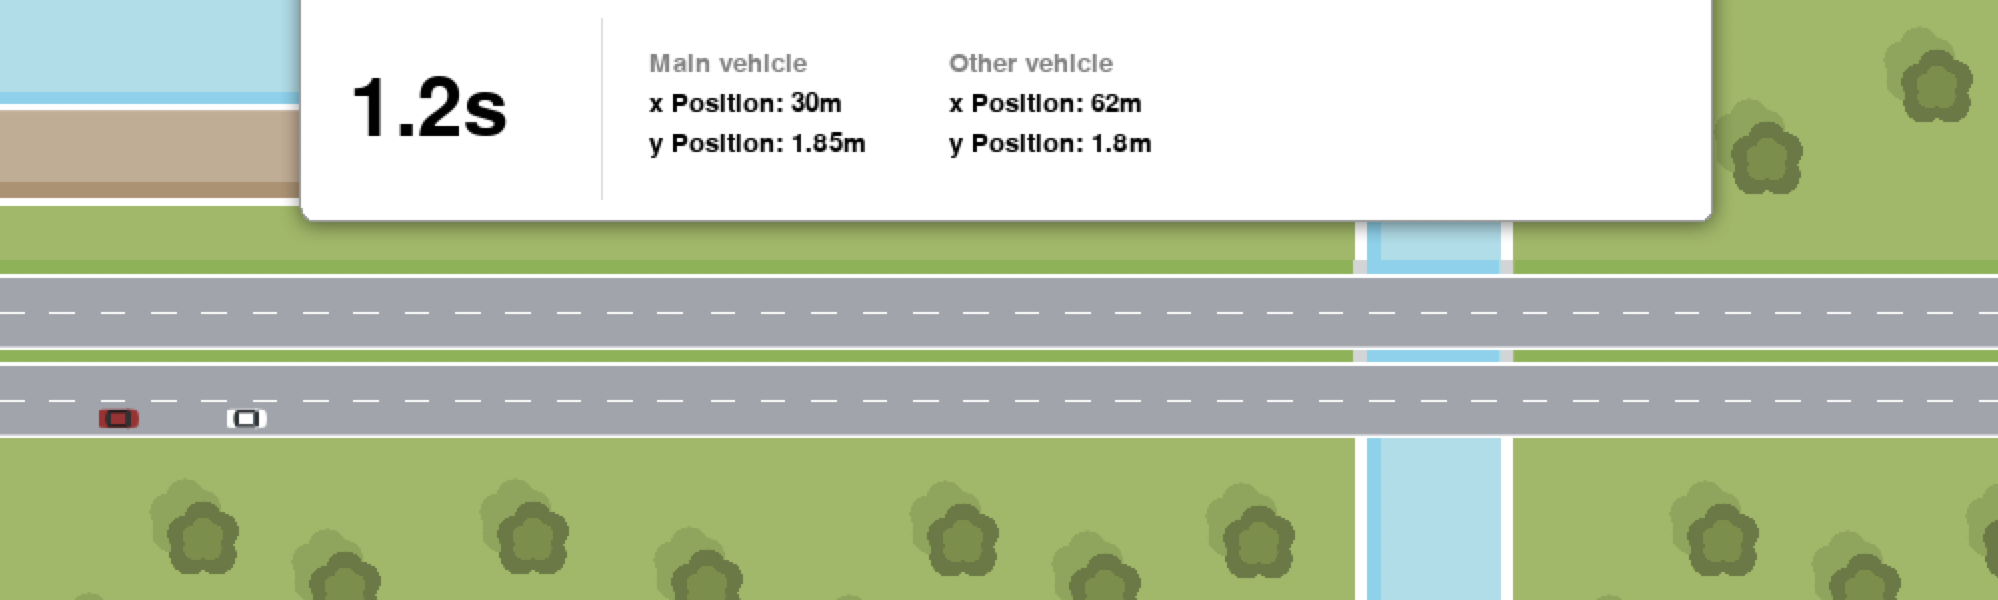
\includegraphics[width=1\textwidth]{snap_1.png}
\end{subfigure}\\ \vspace{2px}
\begin{subfigure}{0.75\textwidth}
  \centering
  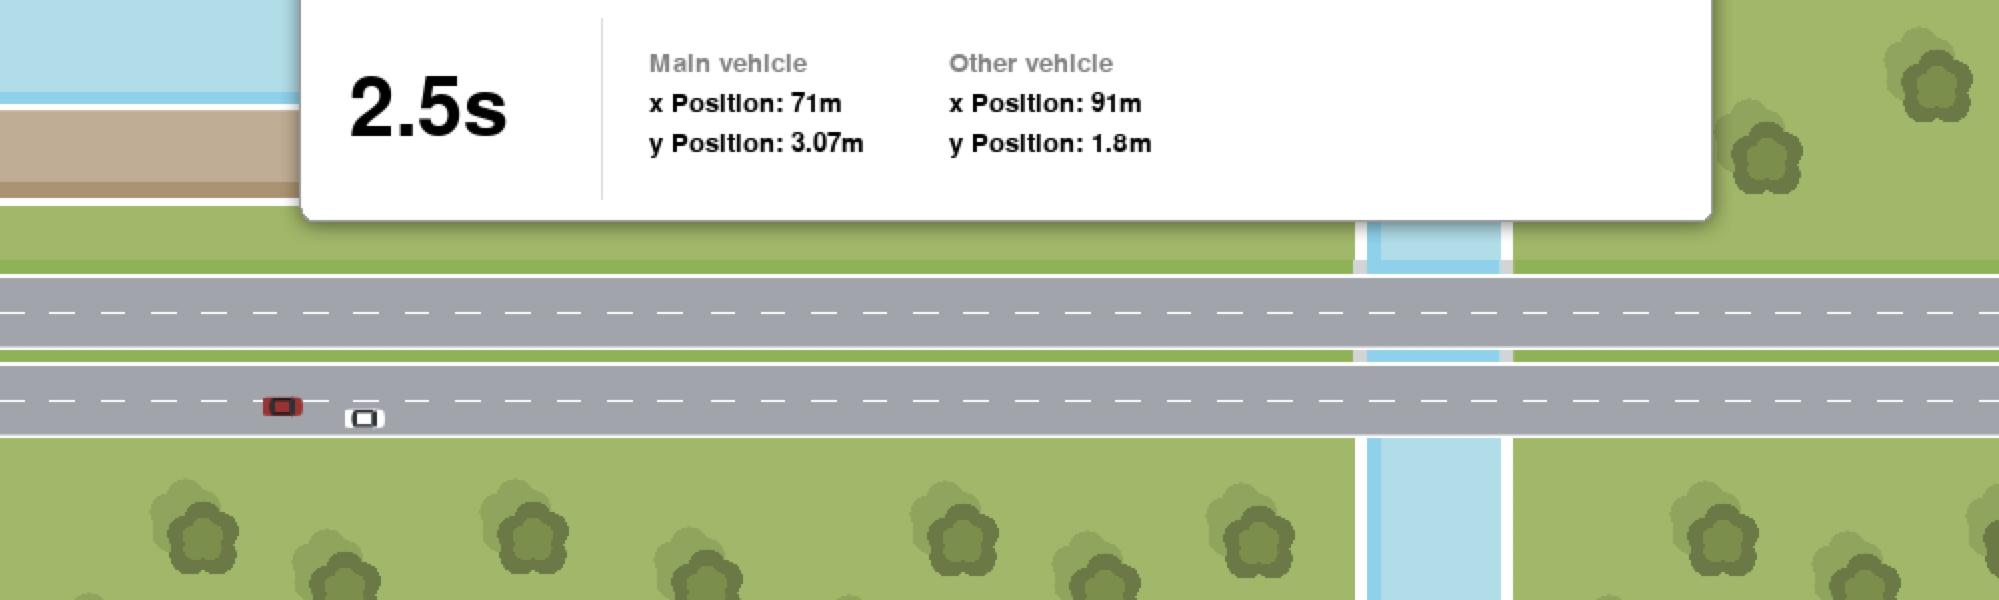
\includegraphics[width=1\linewidth]{snap_2.png}
\end{subfigure} \\ \vspace{2px}
\begin{subfigure}{0.75\textwidth}
  \centering
  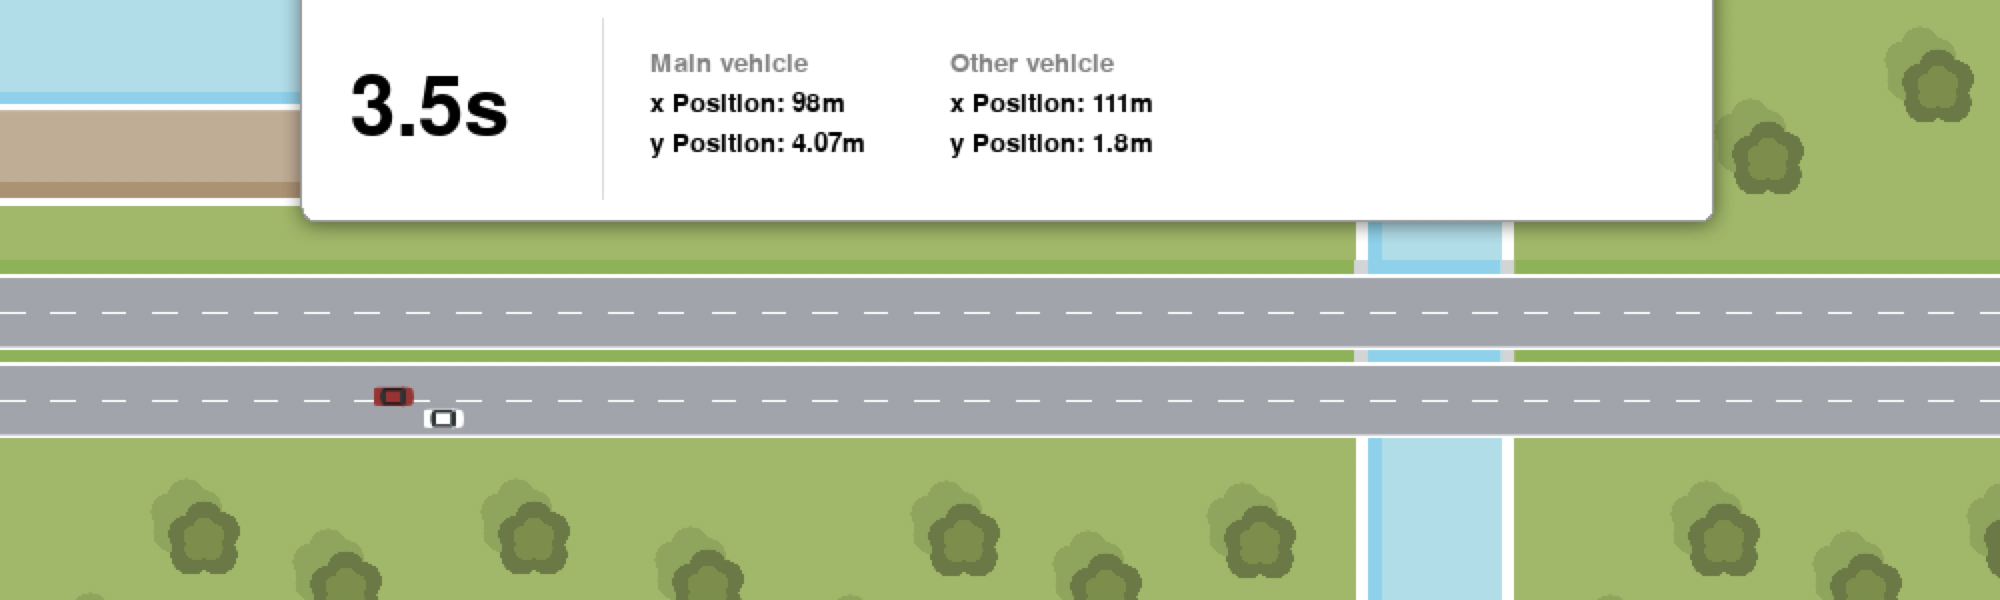
\includegraphics[width=1\linewidth]{snap_3.png}
\end{subfigure} \\ \vspace{2px}
\begin{subfigure}{0.75\textwidth}
  \centering
  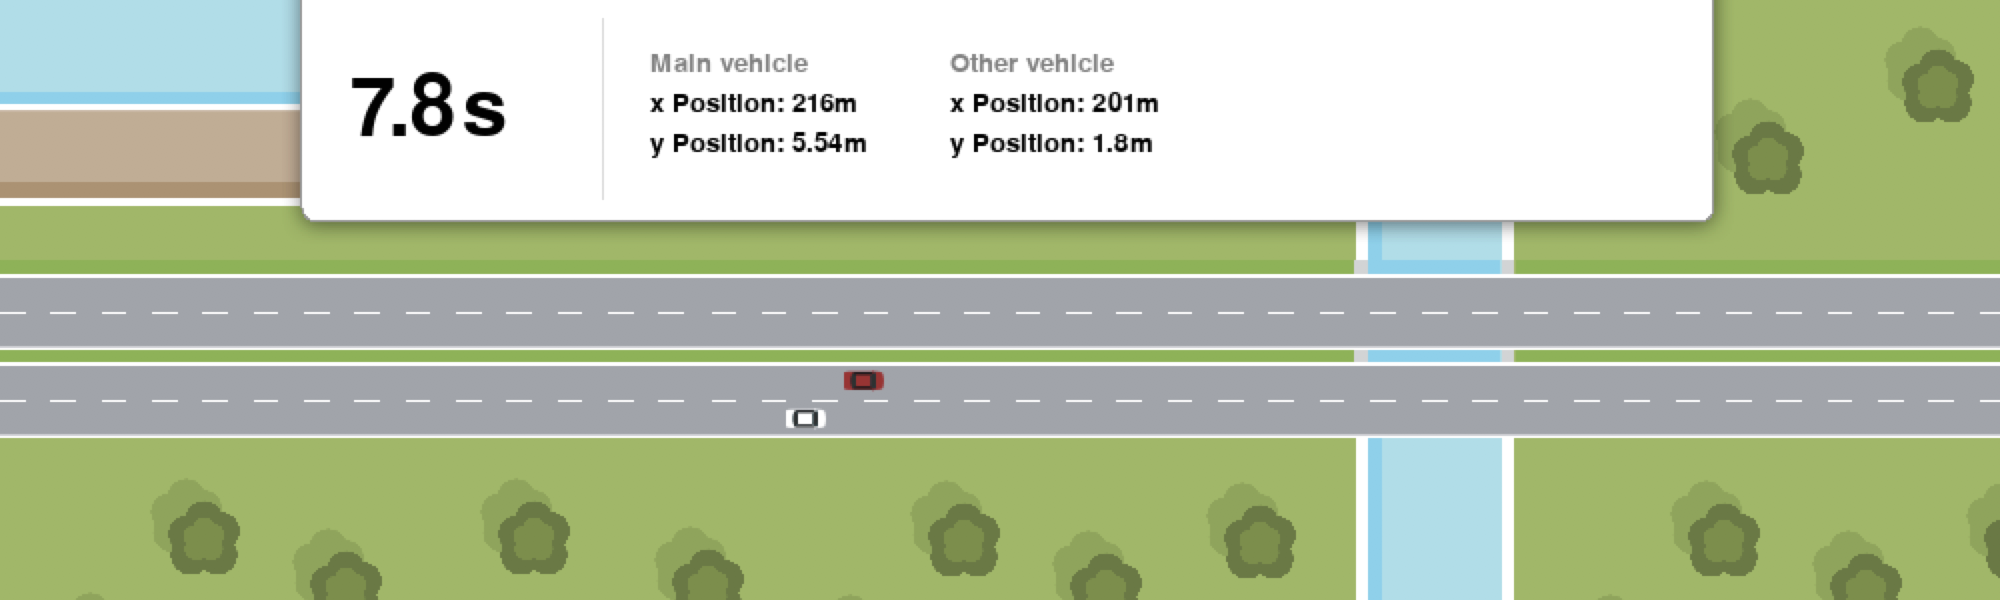
\includegraphics[width=1\linewidth]{snap_4.png}
\end{subfigure} \\ \vspace{2px}
\begin{subfigure}{0.75\textwidth}
  \centering
  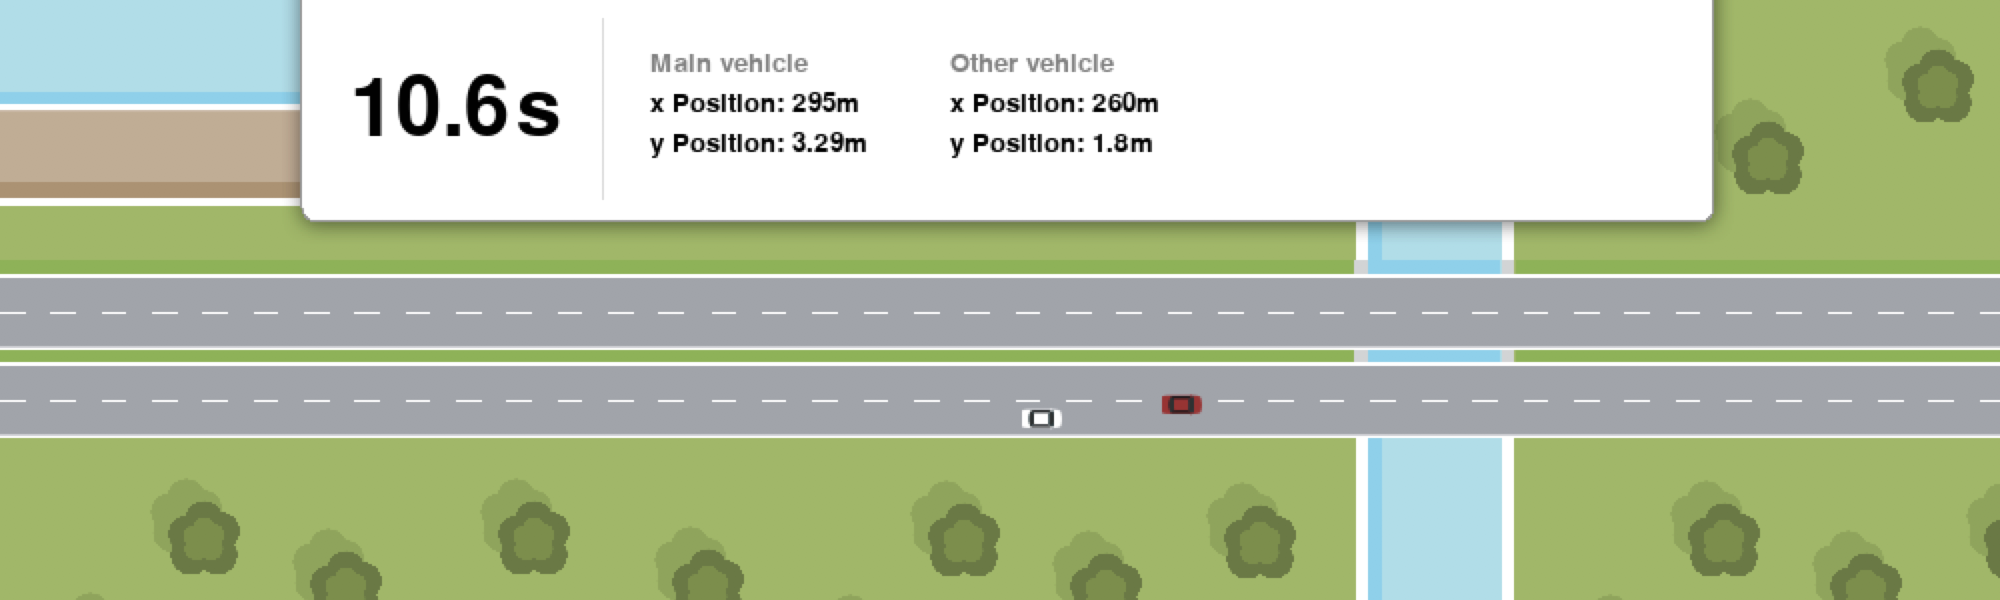
\includegraphics[width=1\linewidth]{snap_5.png}
\end{subfigure} \\ \vspace{2px}
\begin{subfigure}{0.75\textwidth}
  \centering
  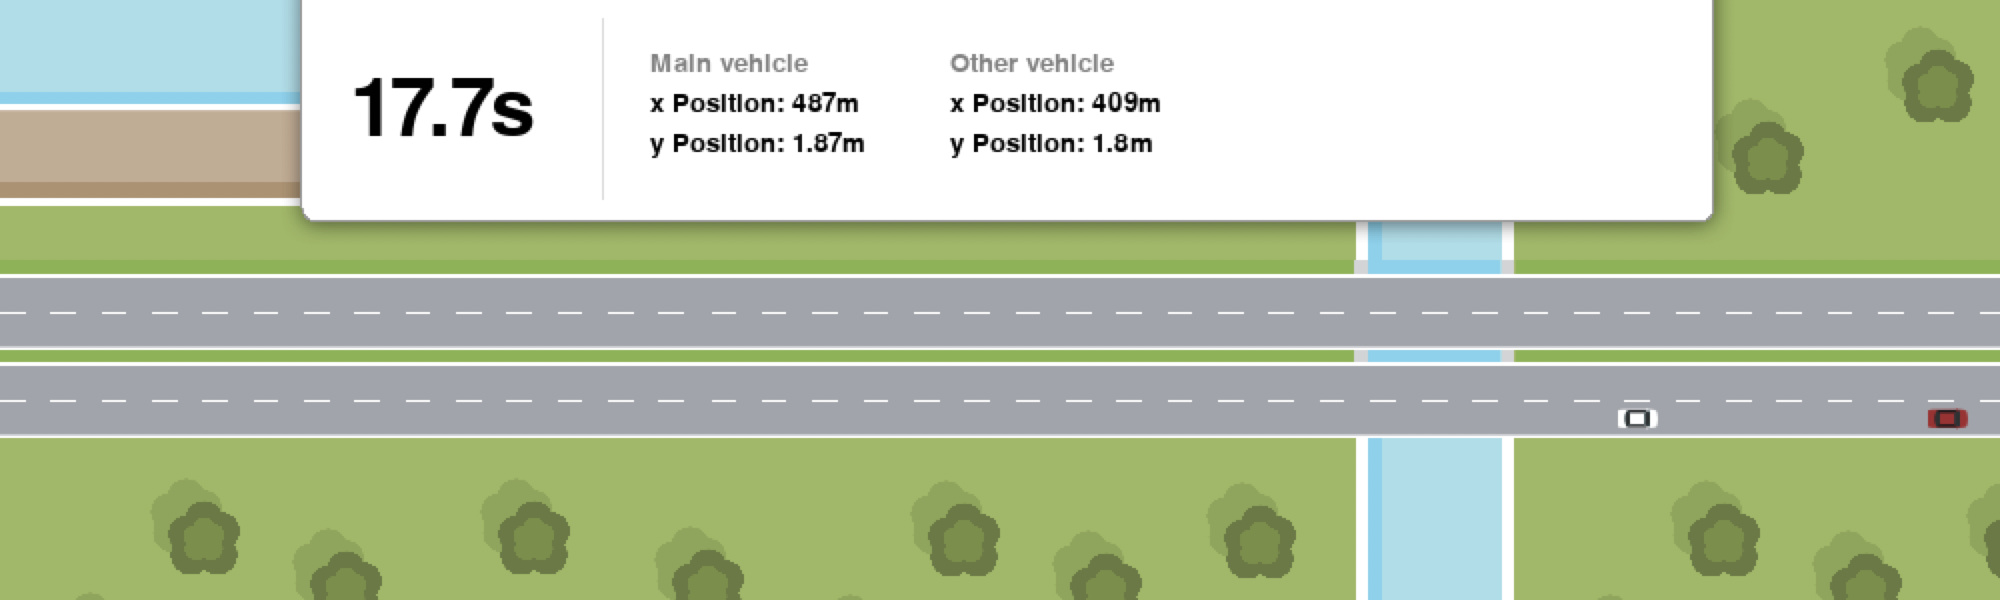
\includegraphics[width=1\linewidth]{snap_6.png}
\end{subfigure}
\caption{Snapshots of the simulator for one of the paths in the scenario $(d_{type}, v, v_1, x_{1,0}) = (3, 28, 21, 38)$.}
\label{fig:example_sim}
\end{figure}



\chapter{Advanced Driver Assistance Systems}
\label{sec:adas}

This chapter explores and compares several ideas for assistance systems which can be implemented on top of the human driver model generated in the previous one. It starts by tackling the design of the system in terms of the placement in the existing module based model and the capabilities within it, following an incremental approach (considering the limitations of the vehicle and drivers). It then performs a comparison of the different approaches using two distinct test cases and it concludes which ADAS performs the best (within reasonable assumptions). This solution is then evaluated and compared to the human driver in Chapter~\ref{sec:results}.

\section{Driver Assistance System Design}

One of the aims of this dissertation is to obtain correct-by-construction driver assistance systems. As such, the design of the assistance system in this context corresponds mostly to determining which actions are available to the system at each state (the model becomes an MDP), and then performing synthesis using adequate properties. It should be noted that these actions must be realistic in nature, otherwise the obtained assistance system would prove to be useless in a real-world scenario - and usefulness is the end goal in terms of deployment. Figure~\ref{fig:adas_possibilities} presents the underlying assumptions of where the system would lie in the environment, which influences the possibilities in terms of the design.

\vspace{1em}
\begin{figure}[h]
    \centering
    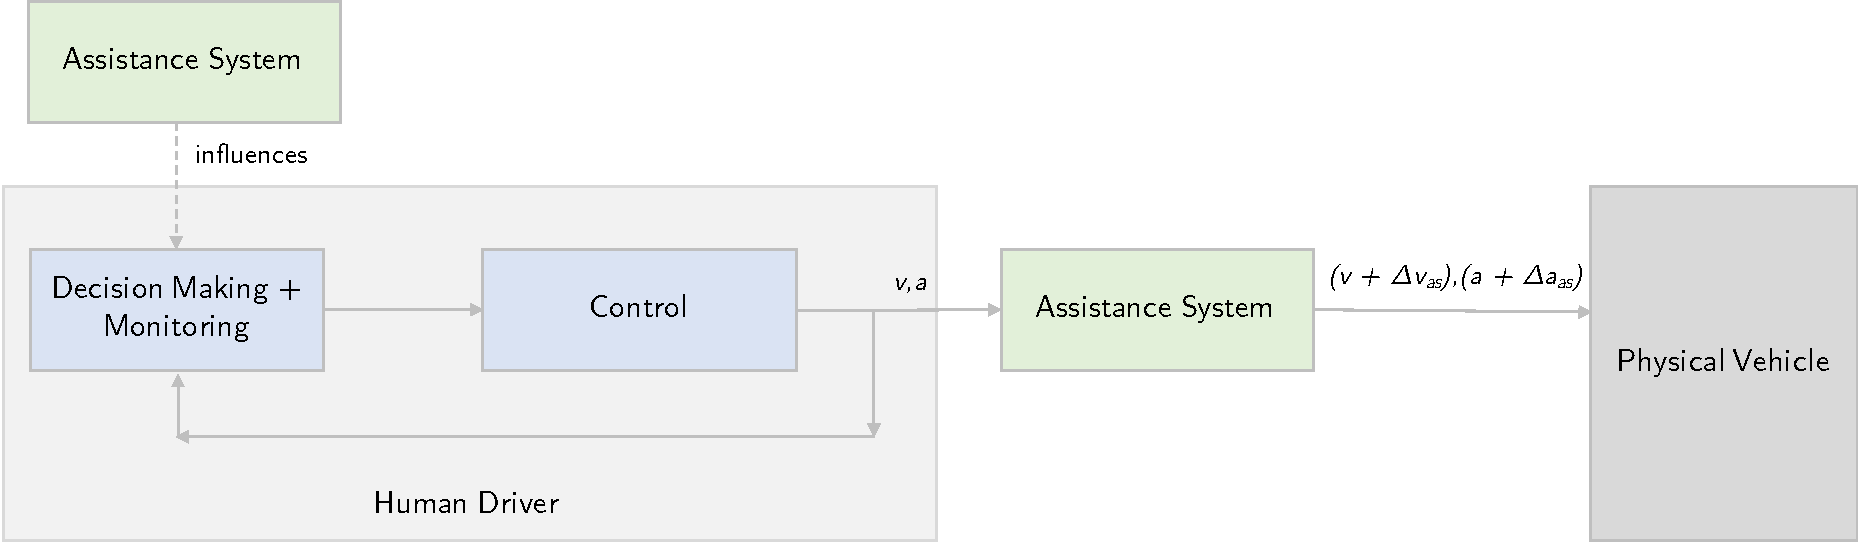
\includegraphics[width=1\textwidth]{adas_possibilities.pdf}
    \caption{Overview of the system with the possibilities of the ADAS intervention.}
    \label{fig:adas_possibilities}
\end{figure}

It is assumed that the assistance system can not change the decision making (as it is a human cognitive process), but it can influence it to a certain degree through suggestion. This would be the ideal way of implementing the ADAS, as it would not require any intervention in the physical systems of the vehicle. Therefore, the first possibilities explored are based on this option. However, in the interest of safety and efficiency, incremental control based options are also developed, both at the level of linear acceleration (influencing $a$ through $\Delta a_{as}$), as well as at the level of steering control (by influencing $v$ and $a$ through $\Delta v_{as}$ and $\Delta a_{as}$, respectively). 

\subsection{Decision Making-based ADAS}

\subsubsection{Decision Making with Fully Compliant Drivers}

At the decision making level, the human driver model considered has two options: it either changes lanes, or it does not. These options can be influenced using suggestions (e.g. through visual or auditive cues) which can lead to either one or the other being taken. Salvucci in \cite{salvucci_1} does not consider accelerating and decelerating as part of the decision making because he argues they happen instinctively and therefore they should be exclusively part of the control. However, if a driver can be influenced to make a conscious decision to decelerate, for example, through the driver assistance system, then there is an argument for including this action in the decision making. Thus, a 3-option ADAS was designed, where an action $\alpha$ is defined as:

\begin{equation}
	\alpha \in A := \{(lc) \vee (\neg lc \wedge a = a_p) \vee (\neg lc \wedge a = a_d)\}
\end{equation}

where $lc$ corresponds to the decision to perform a lane change, $a$ is the acceleration in the next state, $a_p$ is the acceleration the vehicle is currently holding and $a_d$ is a constant value for deceleration that a driver applies when suggested to decelerate. In this dissertation, it was assumed that $a_d = -1$ (minimum decelerating value).

Considering that the drivers are fully compliant with the suggestions given by the system, the decision making at each step can be replaced by the all the possible actions, obtaining an MDP with three choices at this level. The code presented in Appendix~\ref{sec:adas_pdm} corresponds to the implementation of a generator for this ADAS.

\subsubsection{Decision Making with Partially Compliant Drivers}

In the case of the ADAS previously designed, it is assumed that humans will not only follow all the suggestions, but they will comply with them fully and immediately after they are received (within the same ACT-R cycle in the decision making). However, this is not a realistic assumption by any means. In fact, people are more prone to following suggestions when these align with their original intent, than otherwise. With this in mind, a new solution is presented which more accurately represents the suggestive decision making considered in this section.

In the human driver model, a single action was available for a set of conditions, such that at any decision making state ($actr\_state = 2$) $s$ there would be a value $p$ such that the next state $s'$ could be written as:

\begin{equation}
s' = p: (lC) + (1 - p): (\neg lC \:\&\: a = a_p)
\end{equation}

Consider a factor $\gamma \in [0,1]$ which corresponds to how responsive a driver is to the suggestions given. The following rule can be written for each of the actions $\alpha_i \in A$ of the MDP according to the states $s'_i$ which they lead to:

\begin{equation}
s'_i = \gamma: \alpha_i + (1-\gamma)\cdot p:(lC) + (1-\gamma)\cdot (1-p):(\neg lC \:\&\: a = a_p)
\end{equation}

Given that $\gamma, p \in [0,1]$, the transitions are guaranteed to sum up to one for every case. The decision making with fully compliant drivers corresponds to the case where $\gamma = 1$. The code presented in Appendix~\ref{sec:adas_idm} corresponds to the implementation of a generator for this particular ADAS.

\subsection{Control-based ADAS}

While the decision making under the assumption of fully compliant drivers appears to be a powerful option in terms of safety and liveness, the weakening of the assumption to partially compliant drivers is expected to reduce performance substantially, particularly for lower values of $\gamma$. As such, control based assistance is added on top of the decision making assistance considered for partially compliant drivers, so as to improve performance. It should be noted that this type of assistance does not require human intervention, as per the assumptions noted in Figure~\ref{fig:adas_possibilities}.

\subsubsection{Active Linear Acceleration Control}

Considering the assumptions previously described, active linear acceleration control consists in an incremental addition to the acceleration value proposed by the human in the control module. Assume the acceleration of the vehicle imposed by the human is given in the model by $a \in \{a^{\min},...,a^{\max}\}$. In this module, a value $\Delta a_{as}$ is considered such that:

\begin{equation}
\label{eq:delta_as_rest}
	\Delta a_{as} \in \{\Delta a_{as}^{\min},...,\Delta a_{as}^{\min}\}: \Delta a_{as}^{\min} > a^{\min} \wedge \Delta a_{as}^{\max} < a^{\max}
\end{equation}

and the final acceleration applied to the vehicle becomes (considering as well that $a' \in \{a^{\min},...,a^{\max}\}$):

\begin{equation}
	a'(t) = \max (\min (a(t) + \Delta a_{as}, a^{\max}), a^{\min})
\end{equation}

The restriction to the values of $\Delta a_{as}$ presented in Equation~\ref{eq:delta_as_rest} allows the system to be incremental (i.e. corrective) instead of enforcing the specific values chosen by the control assistance system. This is important to avoid strategies for the control assistance system which sharply contrast in terms of the values chosen, e.g. a strategy which at a certain time chooses an acceleration of $3$ and in the next time step chooses one of $-2$ (not allowed for a small enough range of $\Delta a_{as}$ and according to the linear control abstraction obtained in Chapter~\ref{sec:human_driver}). In this dissertation, it is assumed that $\Delta a_{as} \in \{-1,0,1\}$.

The implementation of such system consists in replacing the existing linear control at each step of the control module by the resulting accelerations of applying all the possible values of $\Delta a_{as}$ to the acceleration decided by the human control module, obtaining an MDP with at most three actions at the linear acceleration control level (and at least two). The code presented in Appendix~\ref{sec:adas_lc} corresponds to the implementation of a generator for this ADAS (with the decision making assistance for partially compliant drivers).

\subsubsection{Active Steering Control}

While linear acceleration control assistance improves safety and liveness, steering assistance can also be improved using incremental velocity and acceleration. 

In \cite{salvucci_1}, Salvucci introduces a control law for the steering angle $\varphi$, as presented in Section~\ref{sec:salvucci}, for a given $k_{far}, k_{near}$ and $k_I$. By changing the values of these constants, different control laws are obtained, which introduce different accelerations and velocities at each time step, mimicking the behaviour of the incremental control previously assumed (i.e. within such a strategy, the difference in acceleration and velocity introduced is the difference between these values for the two control laws at each time step). The value of $\theta_{\max}$ (as defined in Section~\ref{sec:salvucci}), guarantees the feasibility of the movement in terms of the acceleration induced. Thus, actions in this assistance system at the model level correspond to different sets of $(k_{far}, k_{near},k_I)$ available to the ADAS.

In this dissertation, three distinct sets of parameters were considered as possible actions, $(k_{far}, k_{near},k_I) \in \{(15,3,5), (17,3,6), (14.5,3,7)\}$. An example of the simulation for the situation where $o_{lane} = 1$, $d = 20m$, $v = 15m/s$ and $v_1 = 15m/s$ (with the non-probabilistic control) is presented in Figure~\ref{fig:steering_control_ex}.

\begin{figure}[h]
    \centering
    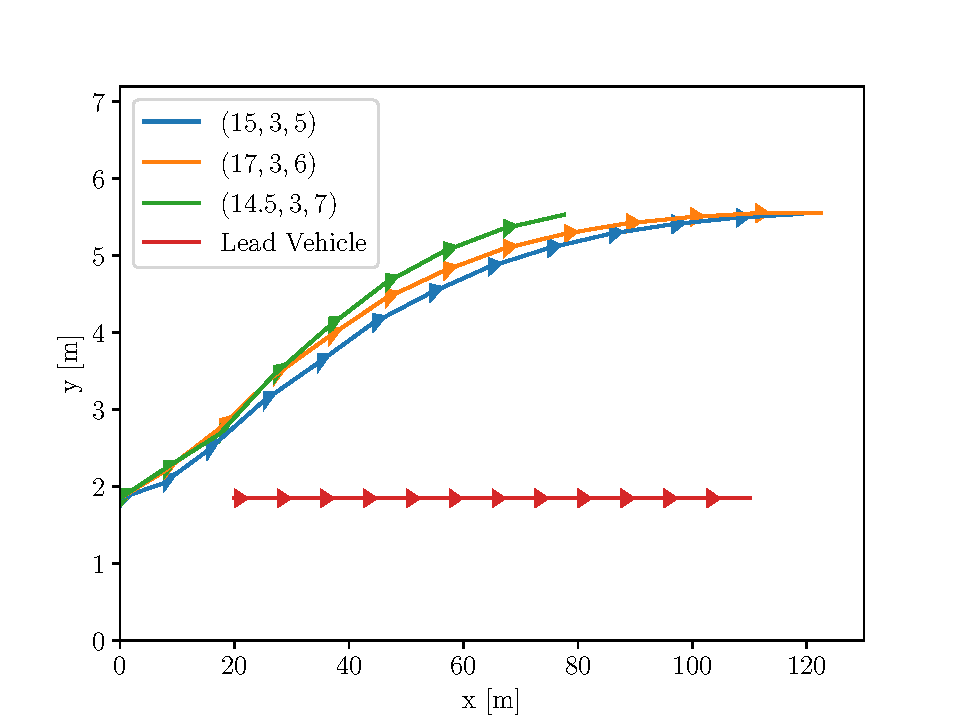
\includegraphics[width=0.9\textwidth]{steering_control_ex.pdf}
    \caption{Example of the simulation of the lane change for $o_{lane} = 1$ (right lane), $d = 20m$, $v = 15m/s$ and $v_1 = 15m/s$ (the legend of each path corresponds to the situation with parameters $k_{far}, k_{near},k_I$, respectively).}
    \label{fig:steering_control_ex}
\end{figure}

Using these values, new look-up tables were obtained with the probability of crashing, the $\Delta x$ and $\Delta T$ incurred and the final velocity of the vehicle in question (following the probabilistic control module presented in Section~\ref{sec:prob_control}) for each origin lane, distance to the other vehicle, velocities of both the vehicle in question and the other vehicle and the parameters of the control law (out of the three possibilities presented). Following the same calculations as shown in Section~\ref{sec:non_prob_control}, the obtained look-up table contains $103,200$ rows.

In terms of implementation, the MDP is obtained through simply reading the three possible actions for lane changing directly from the look-up table, similarly to the human driver model (the difference being the latter only has one option). The code presented in Appendix~\ref{sec:adas_sc} corresponds to the implementation of a generator for this ADAS (with the decision making assistance for partially compliant drivers and active linear acceleration control).

\section{Design Evaluation}

While it would appear to be the case that an ADAS with both decision making and control assistance at the linear acceleration and steering level would be the optimal choice for the driver assistance system, there are no guarantees that this is true. As such, an evaluation and comparison of all the possible designs must be performed in order to determine the best option which can then be compared to the human driver model in Chapter~\ref{sec:results}. To do so, it is necessary to establish multi-objective metrics and some meaningful test cases (as testing all the options would be infeasible).

\subsection{Multi-Objective Metrics}
\label{sec:multi_obj_metrics}

As established in Section~\ref{sec:model_metrics}, safety and liveness are two important metrics which will be used in Chapter~\ref{sec:results} to evaluate the human driver model. Therefore, it makes sense that such properties should be the focus of the synthesis for the driver assistance system. The goal is to minimise the probability of crashing and to maximise the liveness property. This can be obtained using a multi-objective query such as the one below:

\begin{minipage}{\linewidth}
{\vspace{1em}
\begin{lstlisting}
multi(Pmin=? [F crashed], Pmax=? [F (x=length) & (t<T)])
\end{lstlisting}
}
\end{minipage}

for a given constant $T$. Due to the trade-offs between both properties, the model checking of the multi-objective property of the format of the above generates a Pareto curve, where each point on the curve corresponds to optimal achievable values in terms of \texttt{P=? [F crashed]} and \texttt{P=? [F (x=500) \& (t<T)]} under a given strategy. As such, it is possible to compare strategies through the comparison of the Pareto curves obtained for the different ADAS for some test cases.

However, the problem of the safety bias discussed in Section~\ref{sec:live_props} persists through this comparison, and the ideal metric would take into account the conditional probability instead of the unconditional one. Since PRISM does not allow for the model checking of conditional properties, the Pareto curve using the conditional properties needs to be obtained in a different way. At this point, it is important to notice the following equality for a given strategy $\sigma$ in the MDP:

\begin{equation}
	P^{\sigma}_s (\text{\texttt{F crashed}}) = 1 - P^{\sigma}_s (\text{\texttt{F x=length}})
\end{equation}

as long as $p_{\max, s} (\text{\texttt{F (crashed | x = length)}}) = p_{\min, s} (\text{\texttt{F (crashed | x = length)}}) = 1$ (completeness property for the MDP). This is true from the fact that the events crashing and reaching the end are mutually exclusive. Thus, it is possible to write:

\begin{equation}
\label{eq:bayes}
\begin{aligned}
	P^{\sigma}_s (\text{\texttt{F (x=length) \& (t<T)}} \bigmid \text{\texttt{F x=length}}) & = \frac{P^{\sigma}_s (\text{\texttt{F (x=length) \& (t<T)}})}{P^{\sigma}_s (\text{\texttt{F x=length}})} \\
	&  = \frac{P^{\sigma}_s (\text{\texttt{F (x=length) \& (t<T)}})}{1 - P^{\sigma}_s (\text{\texttt{F crashed}})}
\end{aligned}
\end{equation}

It is therefore possible to obtain the Pareto curve with the conditional properties by using Equation~\ref{eq:bayes} on each of the points in the unconditional curve (generating the achievable set through this).

\subsection{Test Cases}

Due to the infeasibility of generating all the possible combinations of test cases, two test cases were considered when comparing the four different ADAS designed in the previous section: the first test case in the scenario $(v, v_1, x_{1,0}) = (21, 19, 70)$ and the second in the scenario $(v, v_1, x_{1,0}) = (30, 22, 50)$. For each of these test cases, the unconditional and conditional Pareto curves for each driver type are presented for a $T$ representative of the scenario and which allows for comparison between the ADAS considered, with Figures~\ref{fig:test_case_1_uncond} and \ref{fig:test_case_1_cond} referring to the first test case, and Figures~\ref{fig:test_case_2_uncond} and \ref{fig:test_case_2_cond} referring to the second test case. In terms of parameters of the model, the same values were used as in the human driver model part of the implementation, and $\gamma$ was set to 0.1.

%For the sake of brevity, the following numbering will be assumed in the captions and discussion of the Pareto curves presented in the test cases:
%
%\begin{enumerate}
%	\item Decision making based ADAS with fully compliant drivers
%	\item Decision making based ADAS with partially compliant drivers (varies with classes of drivers)
%	\item Decision making with partially compliant drivers + linear acceleration control ADAS (varies with classes of drivers)
%	\item Decision making with partially compliant drivers + linear acceleration control + steering control ADAS (varies with classes of drivers)
%\end{enumerate}

%\subsubsection{$v = 21$ m/s, $v_1 = 19$ m/s, $x_{1,0} = 70$ m ($T=20$)}

\begin{figure}[H]
\centering
\begin{subfigure}{0.32\textwidth}
  \centering
  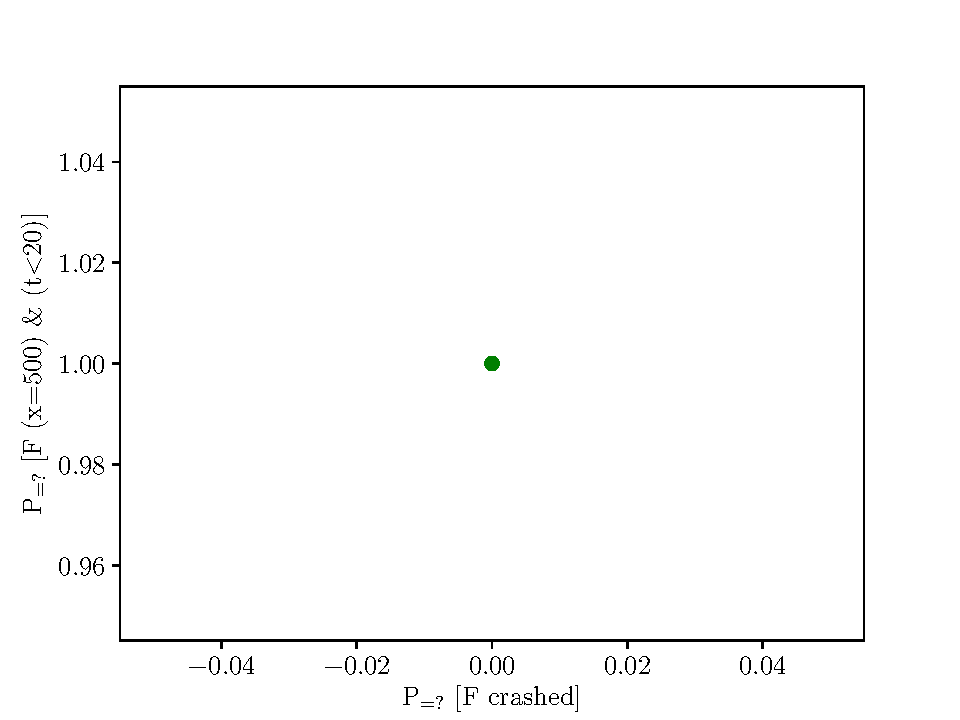
\includegraphics[width=1\textwidth]{test_cases/21_19_70/uncond/1.pdf}
  \subcaption{(1)}
\end{subfigure}\\
\begin{subfigure}{0.32\textwidth}
  \centering
  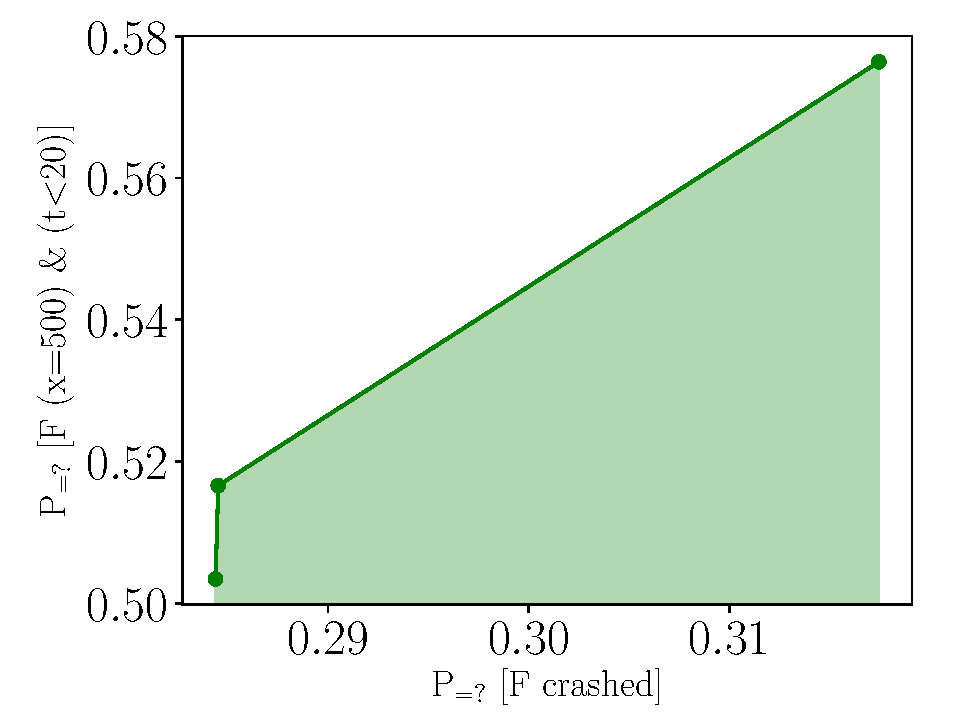
\includegraphics[width=1\textwidth]{test_cases/21_19_70/uncond/2_1.pdf}
  \subcaption{(2) - Aggressive drivers}
\end{subfigure} 
\begin{subfigure}{0.32\textwidth}
  \centering
  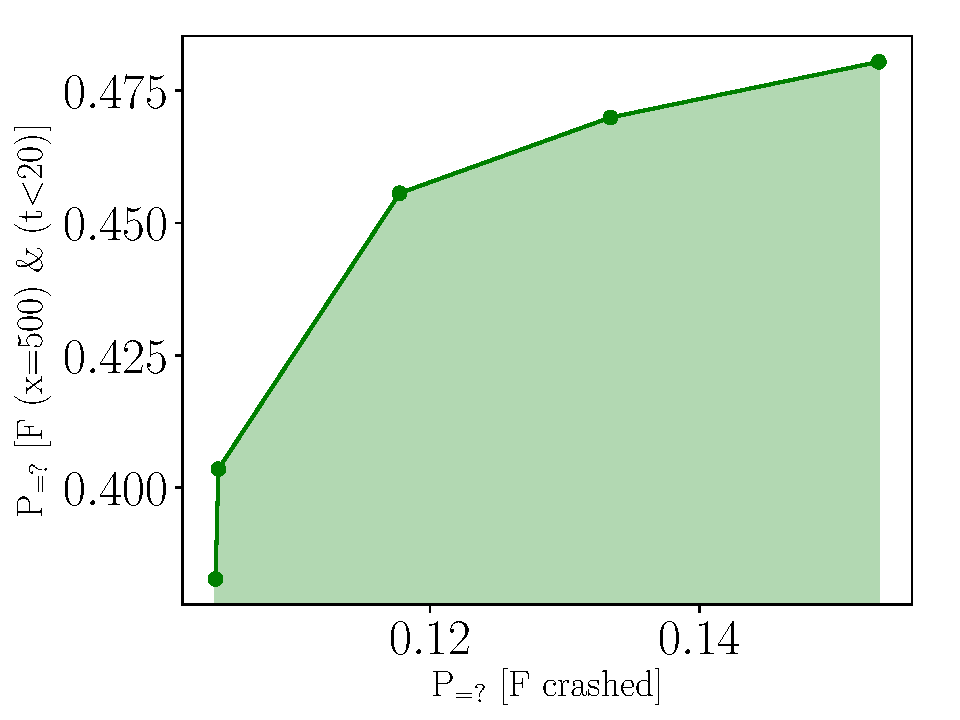
\includegraphics[width=1\textwidth]{test_cases/21_19_70/uncond/2_2.pdf}
  \subcaption{(2) - Average drivers}
\end{subfigure}
\begin{subfigure}{0.32\textwidth}
  \centering
  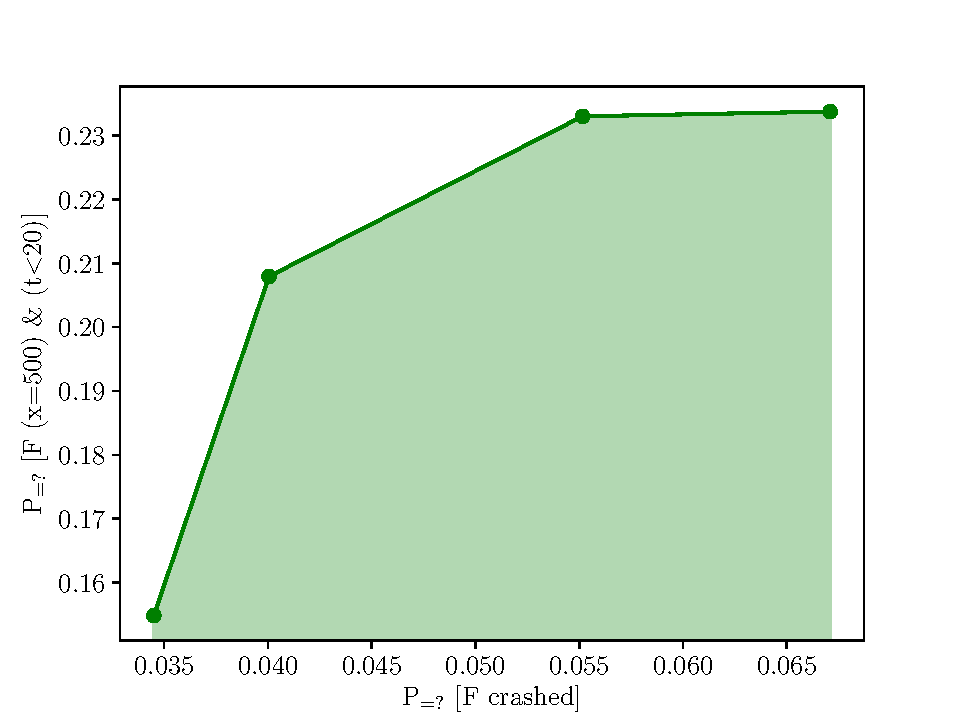
\includegraphics[width=1\textwidth]{test_cases/21_19_70/uncond/2_3.pdf}
  \subcaption{(2) - Cautious drivers}
\end{subfigure}
\begin{subfigure}{0.32\textwidth}
  \centering
  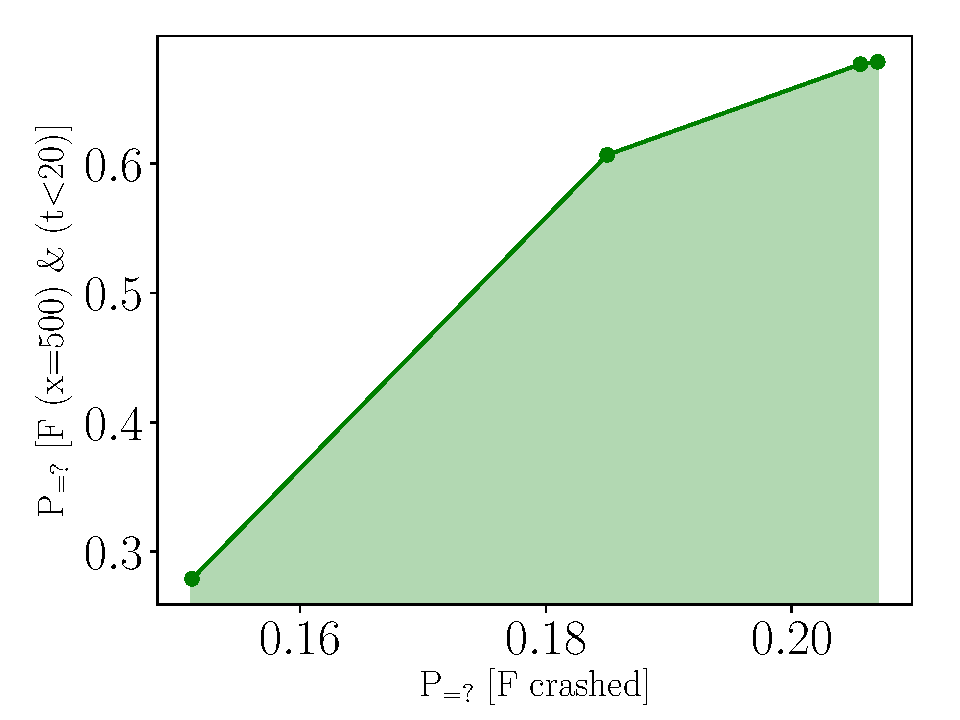
\includegraphics[width=1\textwidth]{test_cases/21_19_70/uncond/3_1.pdf}
  \subcaption{(3) - Aggressive drivers}
\end{subfigure}
\begin{subfigure}{0.32\textwidth}
  \centering
  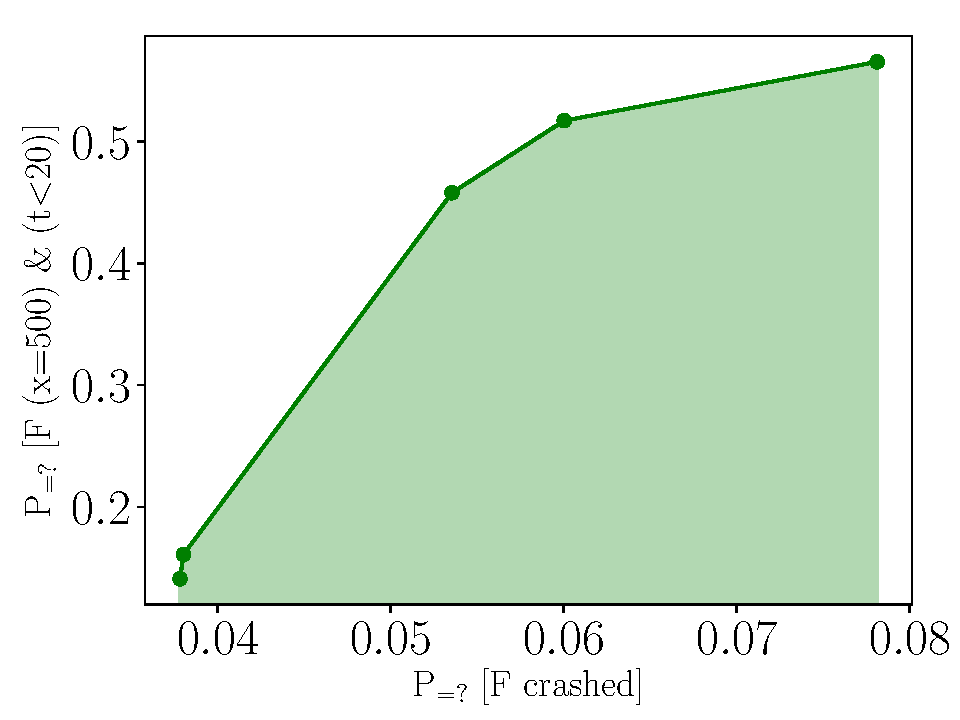
\includegraphics[width=1\textwidth]{test_cases/21_19_70/uncond/3_2.pdf}
  \subcaption{(3) - Average drivers}
\end{subfigure}
\begin{subfigure}{0.32\textwidth}
  \centering
  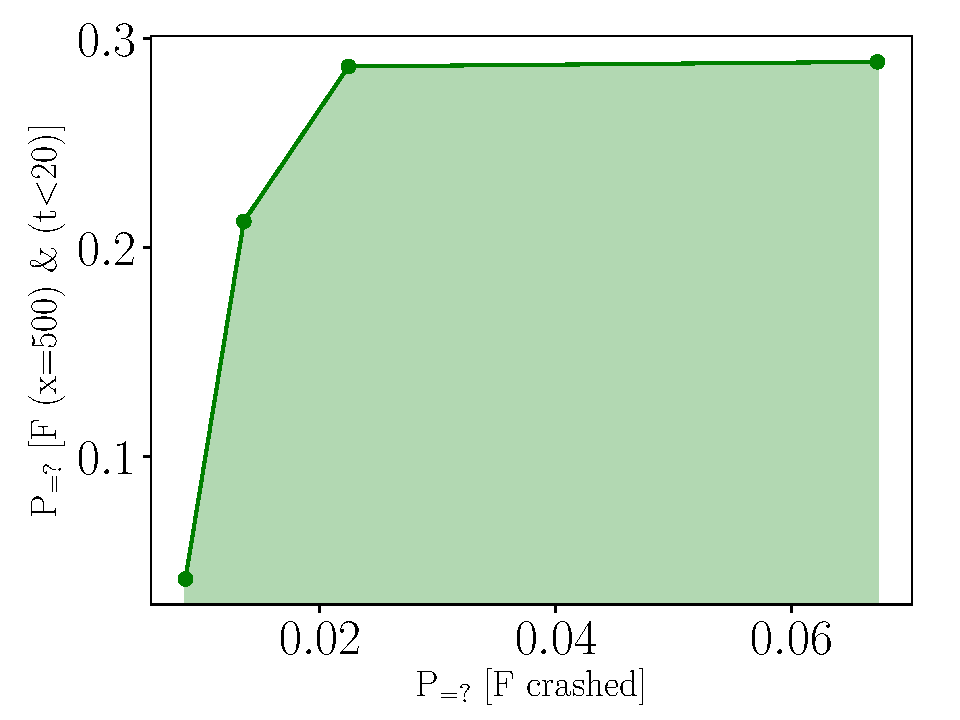
\includegraphics[width=1\textwidth]{test_cases/21_19_70/uncond/3_3.pdf}
  \subcaption{(3) - Cautious drivers}
\end{subfigure}
\begin{subfigure}{0.32\textwidth}
  \centering
  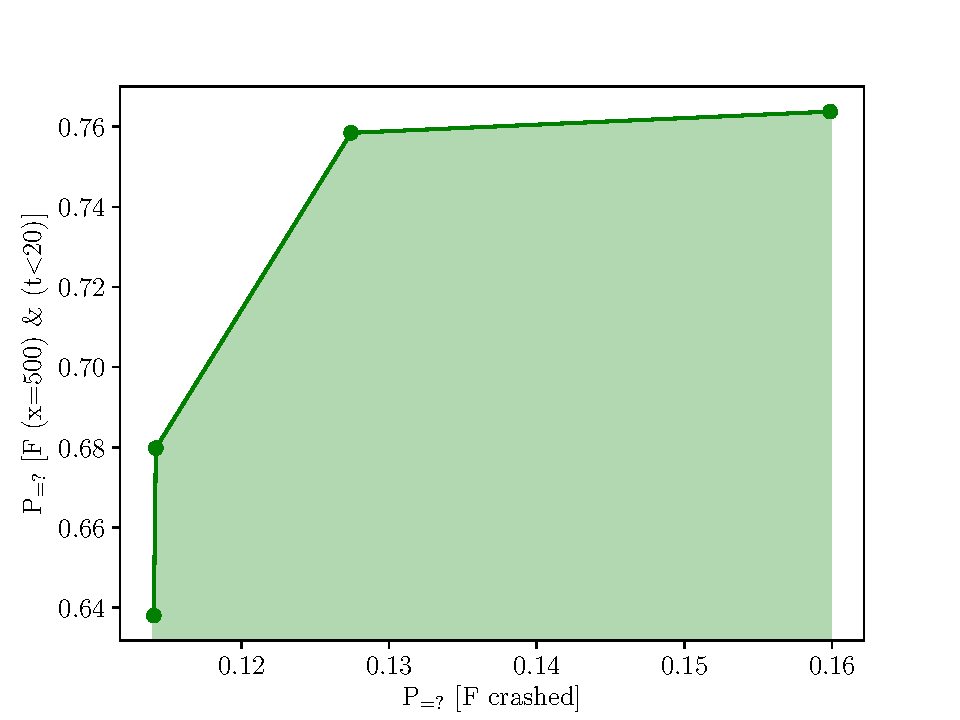
\includegraphics[width=1\textwidth]{test_cases/21_19_70/uncond/4_1.pdf}
  \subcaption{(4) - Aggressive drivers}
\end{subfigure} 
\begin{subfigure}{0.32\textwidth}
  \centering
  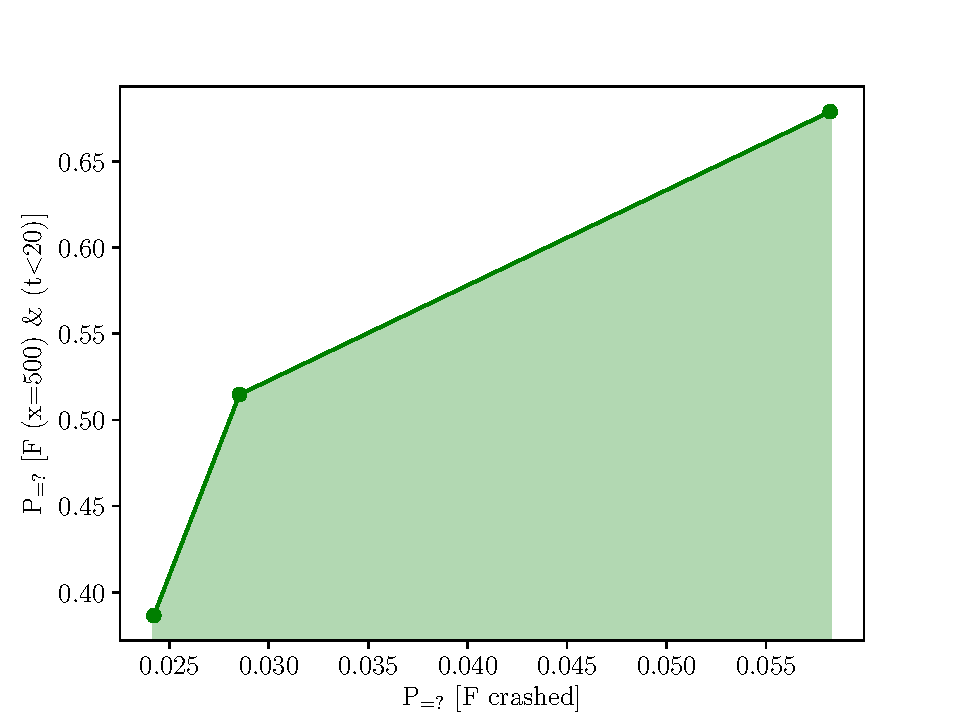
\includegraphics[width=1\textwidth]{test_cases/21_19_70/uncond/4_2.pdf}
  \subcaption{(4) - Average drivers}
\end{subfigure}
\begin{subfigure}{0.32\textwidth}
  \centering
  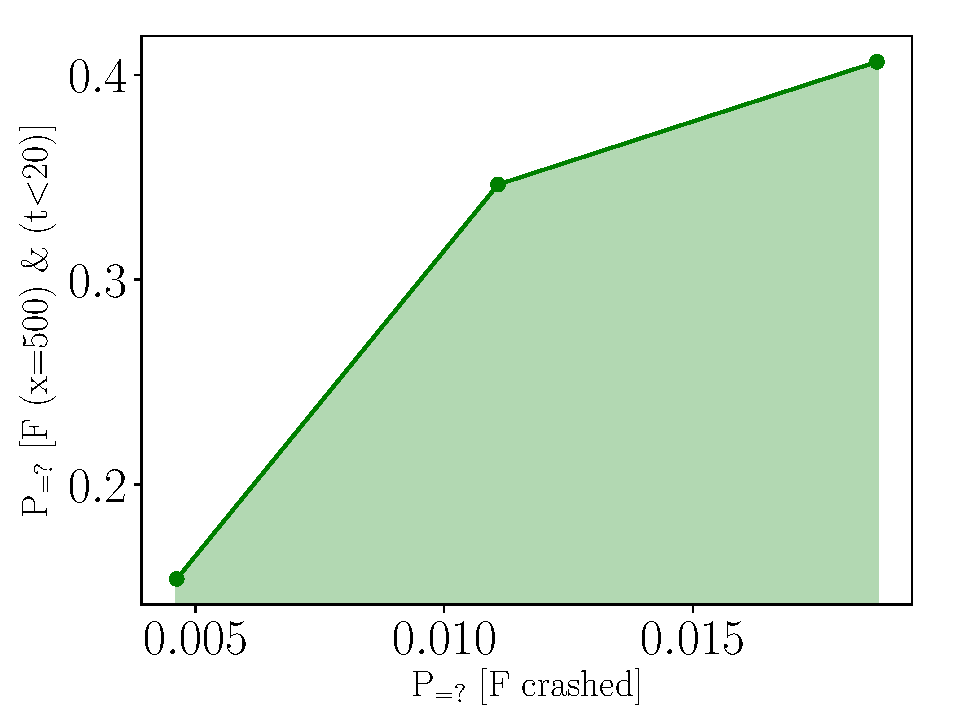
\includegraphics[width=1\textwidth]{test_cases/21_19_70/uncond/4_3.pdf}
  \subcaption{(4) - Cautious drivers}
\end{subfigure}
\caption{Pareto curves of the unconditional properties for the scenario $v = 21m/s$, $v_1 = 19m/s$, $x_{1,0} = 70m$ and for $T = 20$. The ADAS are represented using the following numbering: (1) decision making-based with fully compliant drivers, (2) decision making-based with partially compliant drivers, (3) decision making with partially compliant drivers + linear acceleration control, and (4) decision making with partially compliant drivers + linear acceleration control + steering control.}
\label{fig:test_case_1_uncond}
\end{figure}

%\begin{figure}[H] \ContinuedFloat
%\centering
%\begin{subfigure}{0.49\textwidth}
%  \centering
%  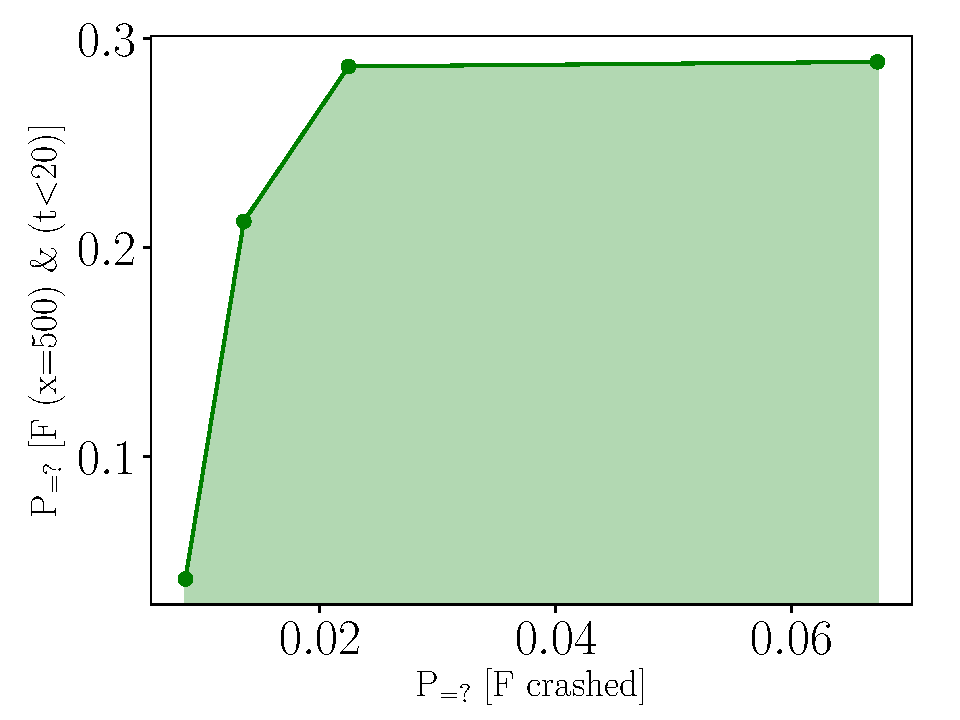
\includegraphics[width=1\textwidth]{test_cases/21_19_70/uncond/3_3.pdf}
%  \subcaption{3 (Cautious drivers)}
%\end{subfigure}
%\begin{subfigure}{0.49\textwidth}
%  \centering
%  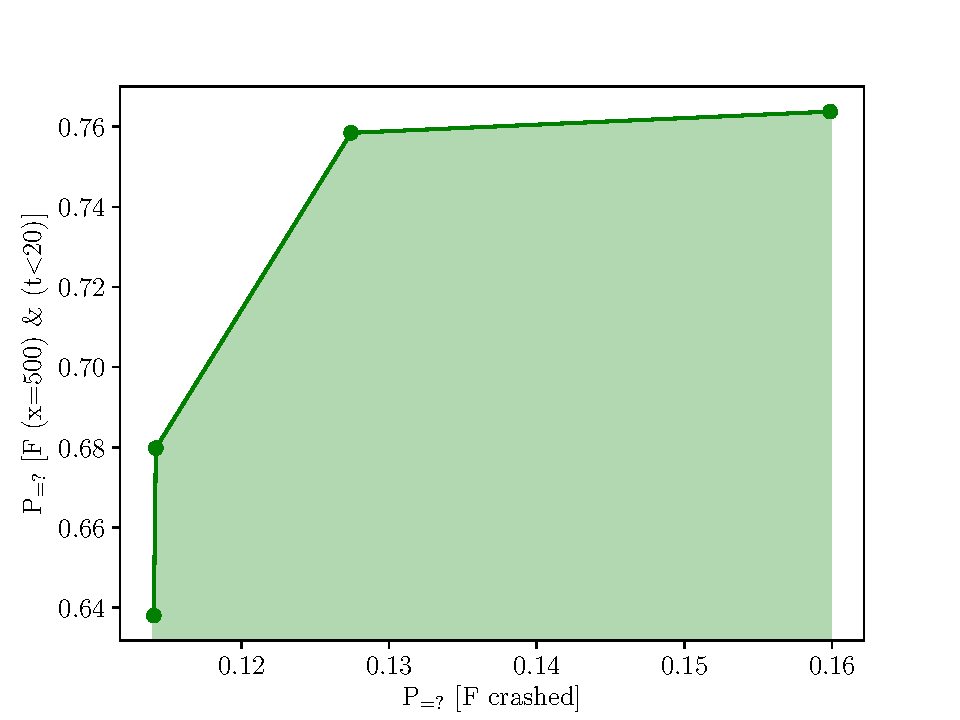
\includegraphics[width=1\textwidth]{test_cases/21_19_70/uncond/4_1.pdf}
%  \subcaption{4 (Aggressive drivers)}
%\end{subfigure} 
%\begin{subfigure}{0.49\textwidth}
%  \centering
%  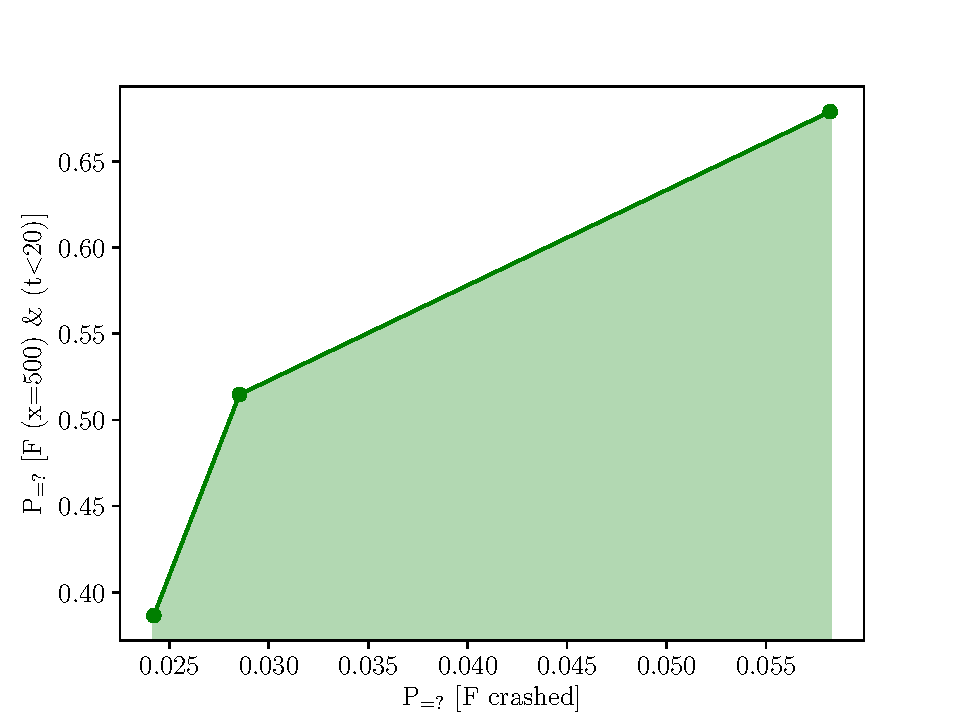
\includegraphics[width=1\textwidth]{test_cases/21_19_70/uncond/4_2.pdf}
%  \subcaption{4 (Average drivers)}
%\end{subfigure}
%\begin{subfigure}{0.49\textwidth}
%  \centering
%  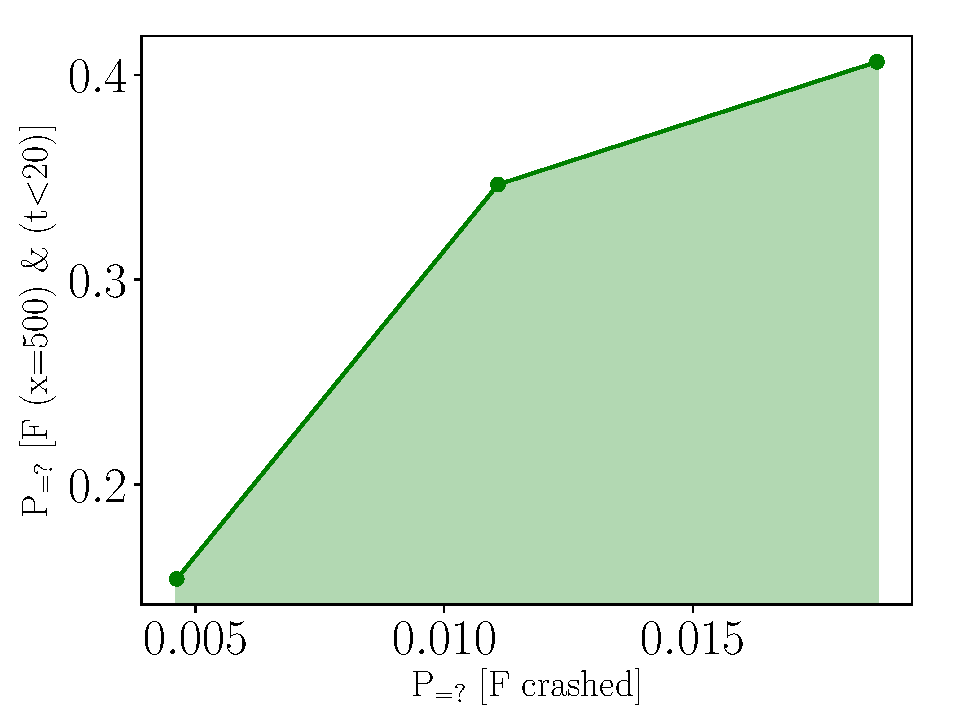
\includegraphics[width=1\textwidth]{test_cases/21_19_70/uncond/4_3.pdf}
%  \subcaption{4 (Cautious drivers)}
%\end{subfigure}
%\caption{Pareto curves for the unconditional properties, for $T = 20$ (cont.).}
%\end{figure}

\begin{figure}[H]
%\vspace{3em}
\centering
\begin{subfigure}{0.32\textwidth}
  \centering
  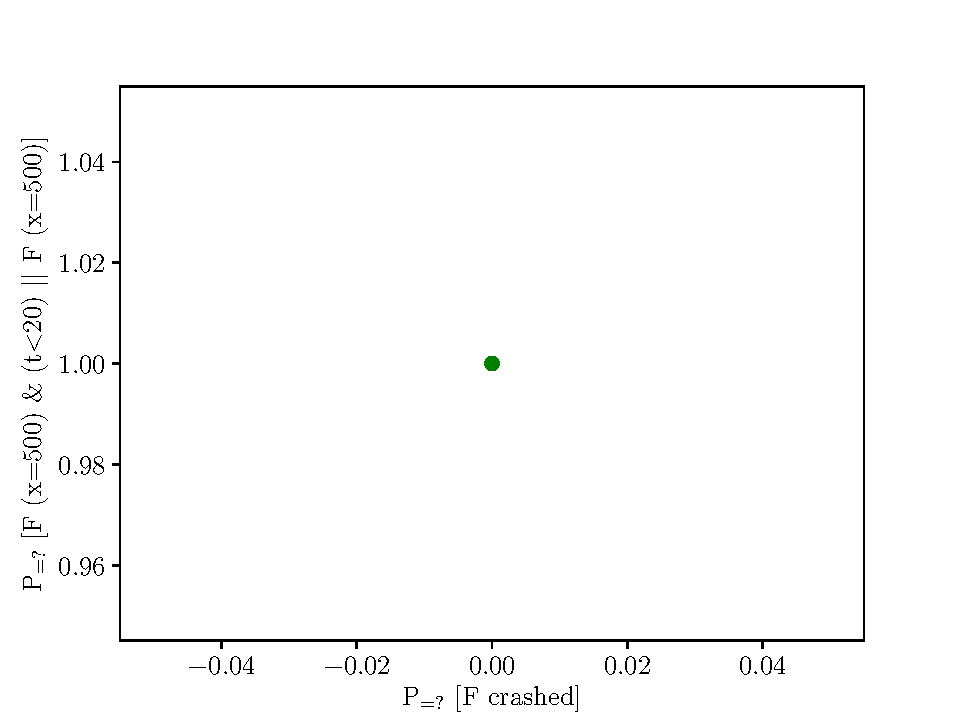
\includegraphics[width=1\textwidth]{test_cases/21_19_70/cond/1.pdf}
  \subcaption{(1)}
\end{subfigure}\\
\begin{subfigure}{0.32\textwidth}
  \centering
  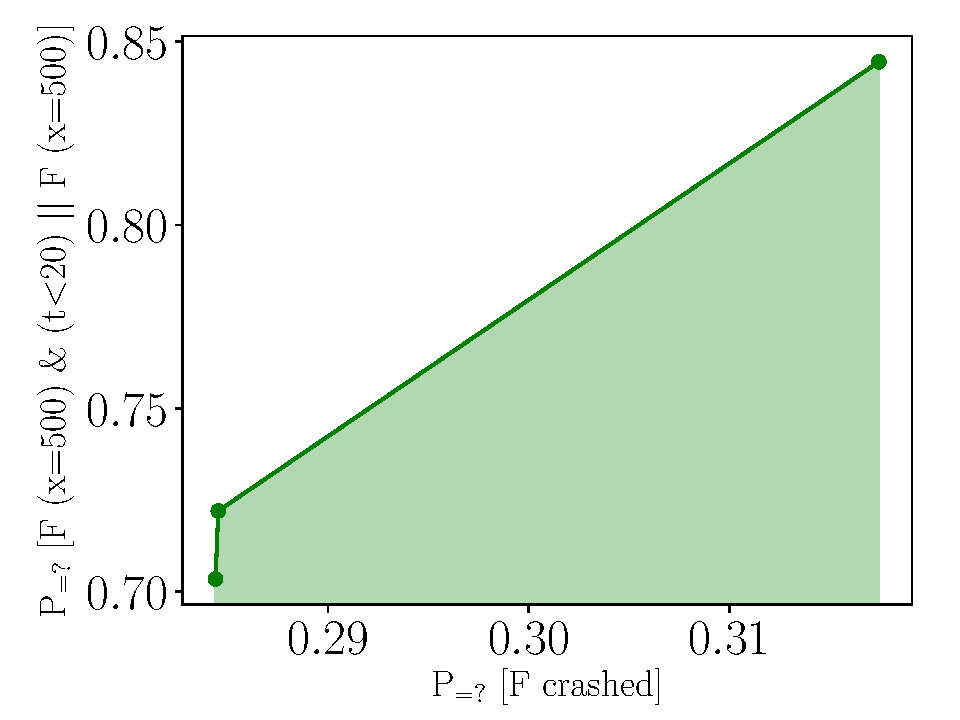
\includegraphics[width=1\textwidth]{test_cases/21_19_70/cond/2_1.pdf}
  \subcaption{(2) - Aggressive drivers}
\end{subfigure} 
\begin{subfigure}{0.32\textwidth}
  \centering
  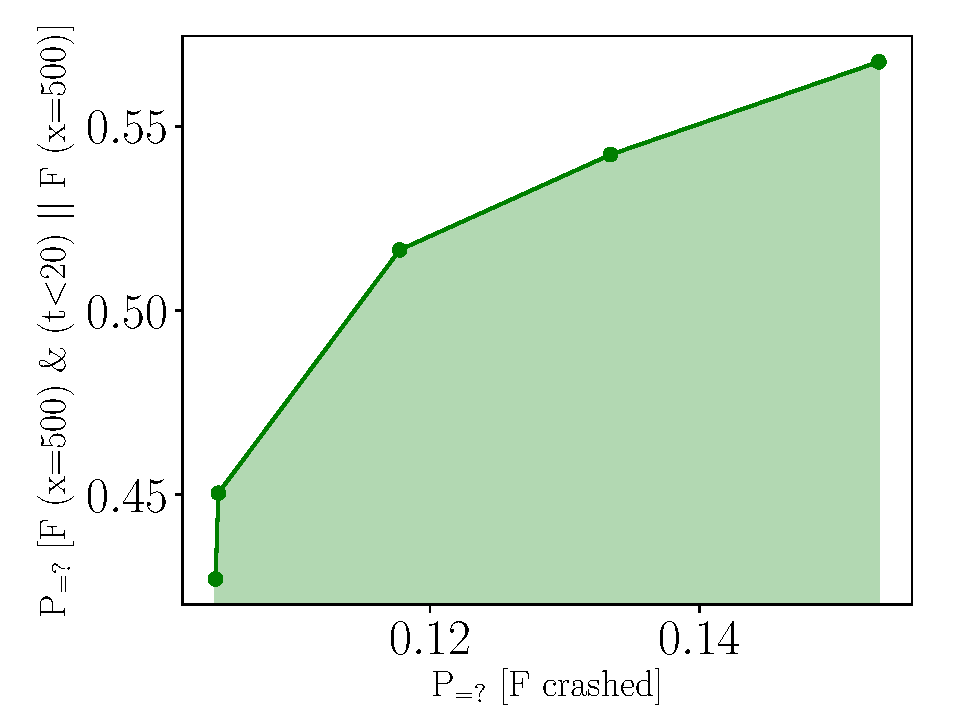
\includegraphics[width=1\textwidth]{test_cases/21_19_70/cond/2_2.pdf}
  \subcaption{(2) - Average drivers}
\end{subfigure}
\begin{subfigure}{0.32\textwidth}
  \centering
  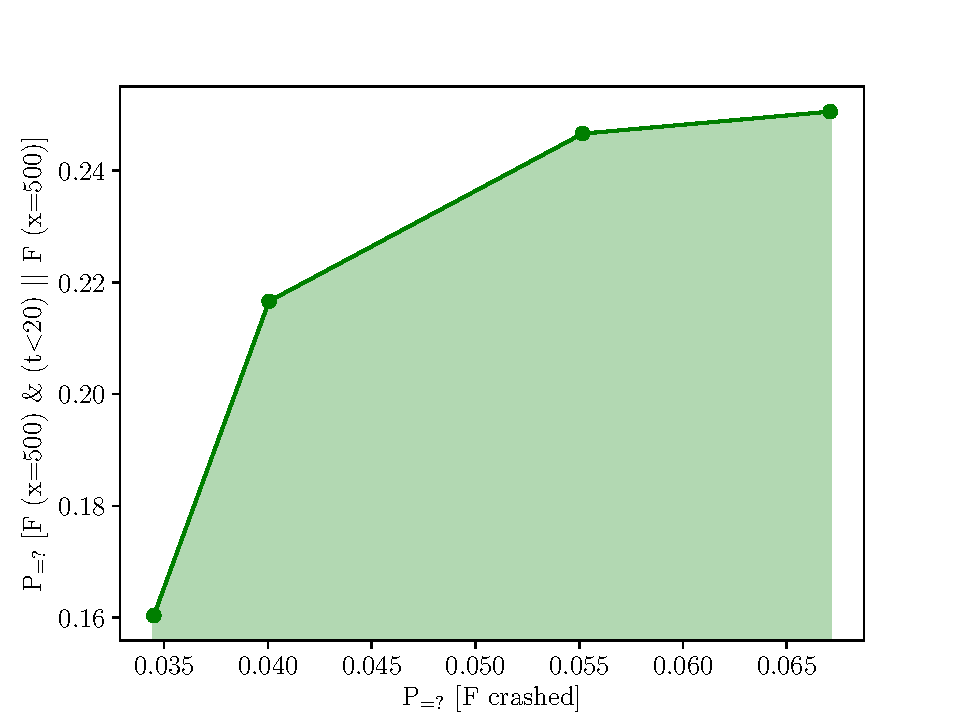
\includegraphics[width=1\textwidth]{test_cases/21_19_70/cond/2_3.pdf}
  \subcaption{(2) - Cautious drivers}
\end{subfigure}
\begin{subfigure}{0.32\textwidth}
  \centering
  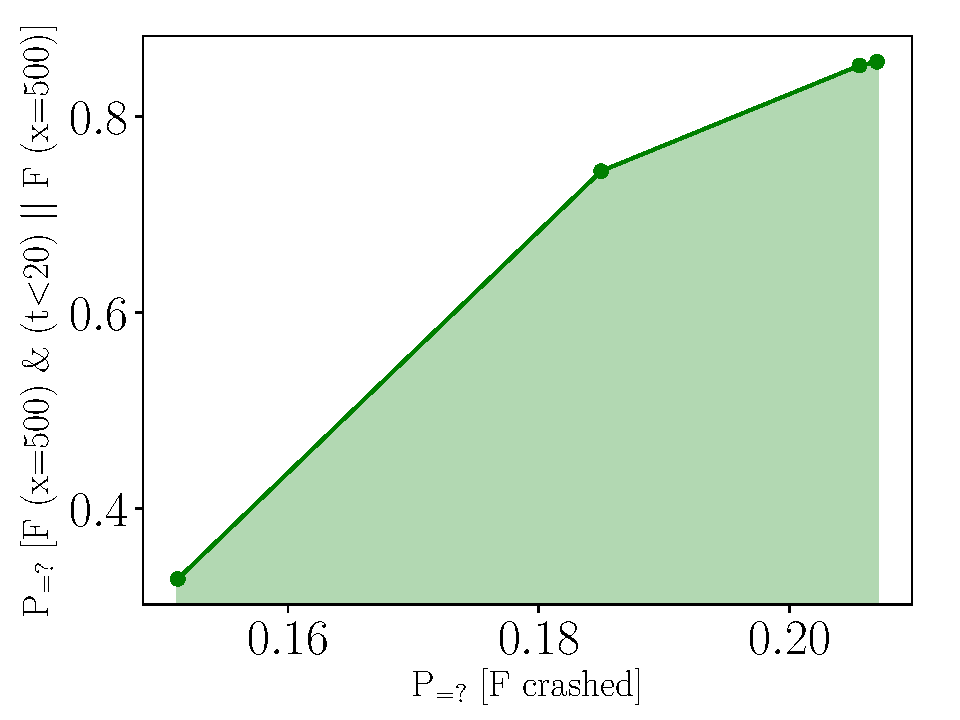
\includegraphics[width=1\textwidth]{test_cases/21_19_70/cond/3_1.pdf}
  \subcaption{(3) - Aggressive drivers}
\end{subfigure}
\begin{subfigure}{0.32\textwidth}
  \centering
  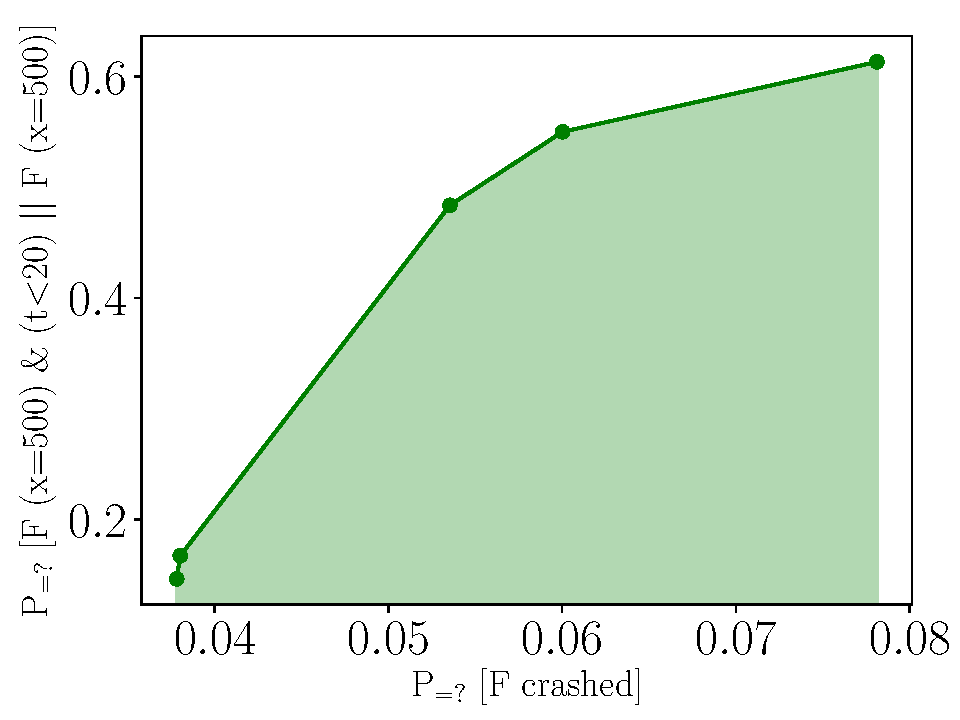
\includegraphics[width=1\textwidth]{test_cases/21_19_70/cond/3_2.pdf}
  \subcaption{(3) - Average drivers}
\end{subfigure}
\begin{subfigure}{0.32\textwidth}
  \centering
  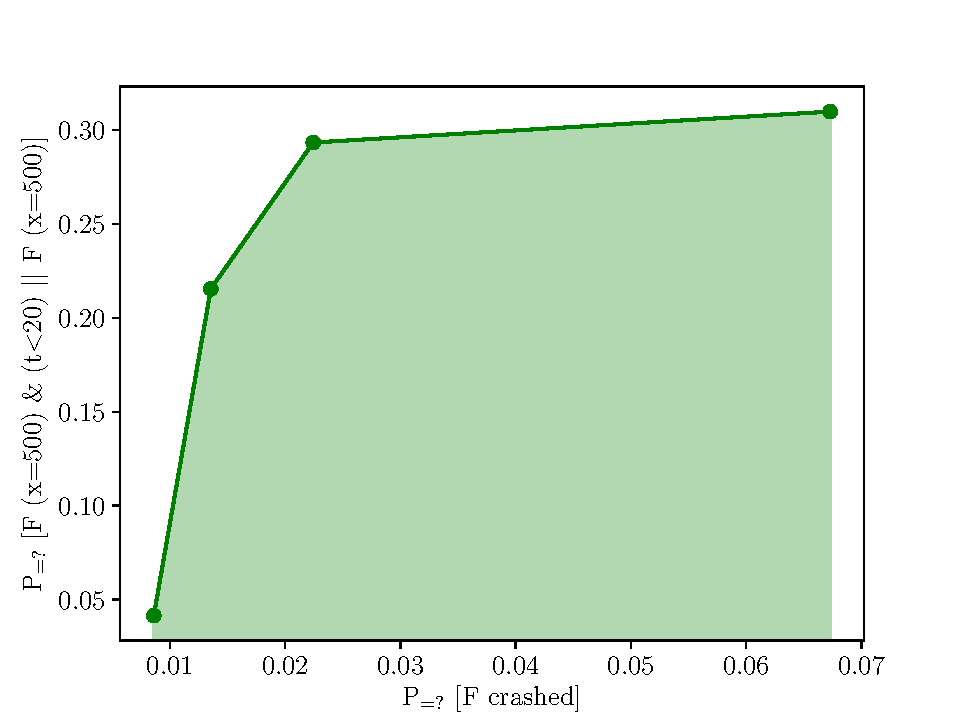
\includegraphics[width=1\textwidth]{test_cases/21_19_70/cond/3_3.pdf}
  \subcaption{(3) - Cautious drivers}
\end{subfigure}
\begin{subfigure}{0.32\textwidth}
  \centering
  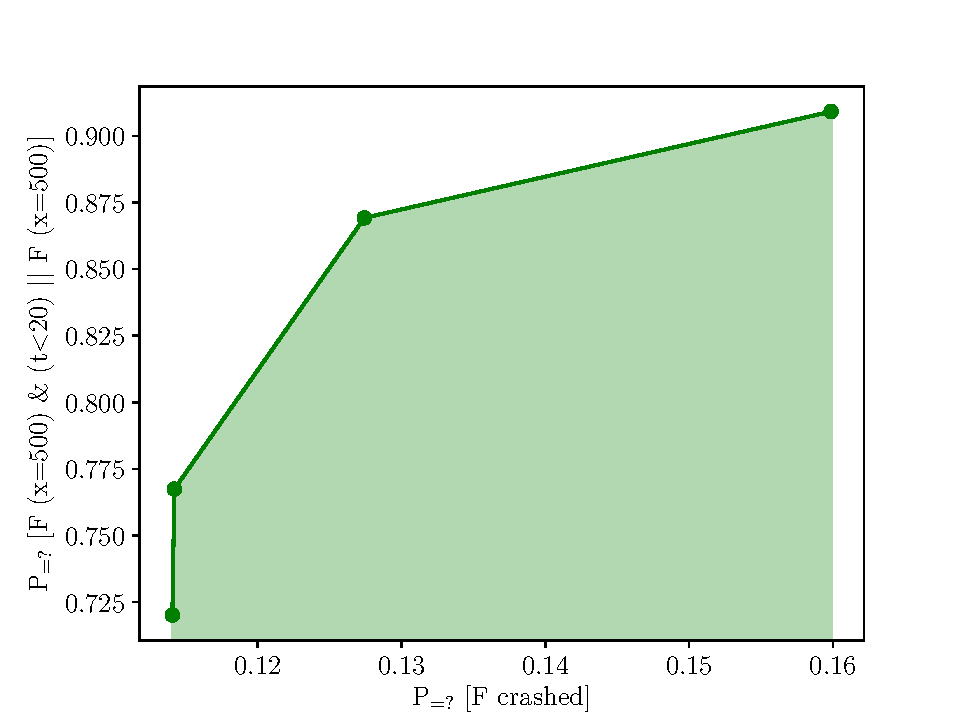
\includegraphics[width=1\textwidth]{test_cases/21_19_70/cond/4_1.pdf}
  \subcaption{(4) - Aggressive drivers}
\end{subfigure} 
\begin{subfigure}{0.32\textwidth}
  \centering
  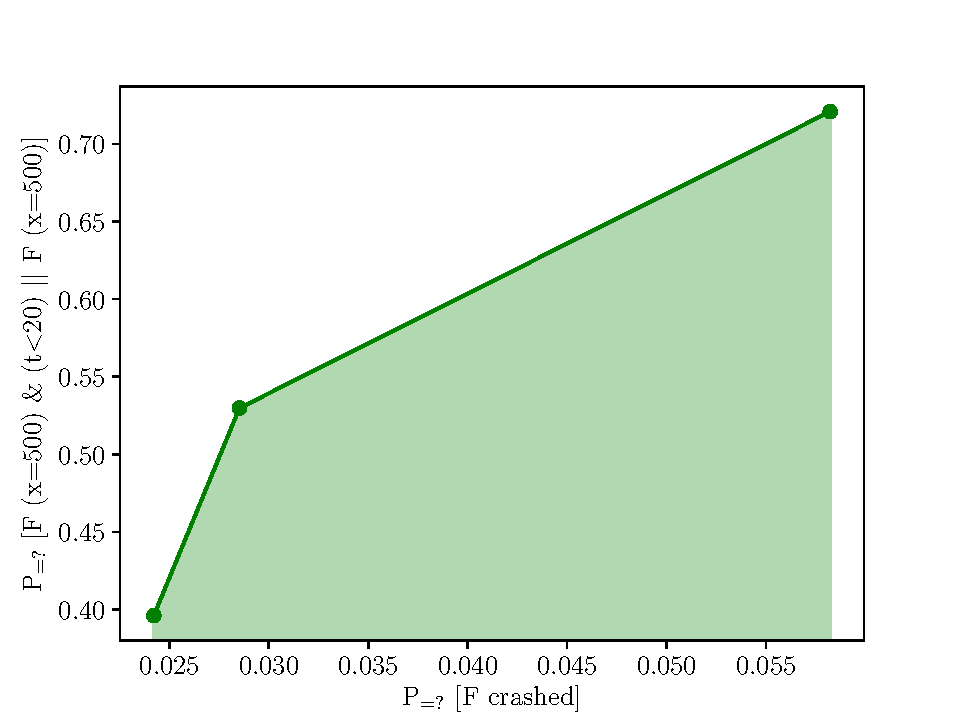
\includegraphics[width=1\textwidth]{test_cases/21_19_70/cond/4_2.pdf}
  \subcaption{(4) - Average drivers}
\end{subfigure}
\begin{subfigure}{0.32\textwidth}
  \centering
  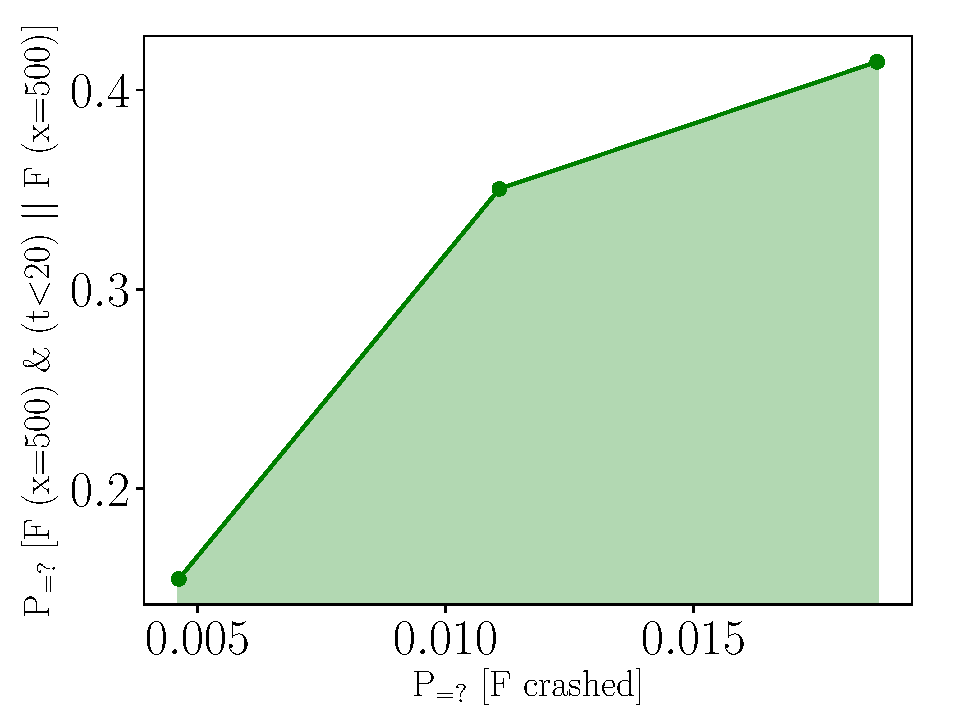
\includegraphics[width=1\textwidth]{test_cases/21_19_70/cond/4_3.pdf}
  \subcaption{(4) - Cautious drivers}
\end{subfigure}
\caption{Pareto curves of the conditional properties for the scenario $v = 21m/s$, $v_1 = 19m/s$, $x_{1,0} = 70m$ and for $T = 20$. The ADAS are represented using the following numbering: (1) decision making-based with fully compliant drivers, (2) decision making-based with partially compliant drivers, (3) decision making with partially compliant drivers + linear acceleration control, and (4) decision making with partially compliant drivers + linear acceleration control + steering control.}
\label{fig:test_case_1_cond}
\end{figure}

%\begin{figure}[H] \ContinuedFloat
%\centering
%\begin{subfigure}{0.49\textwidth}
%  \centering
%  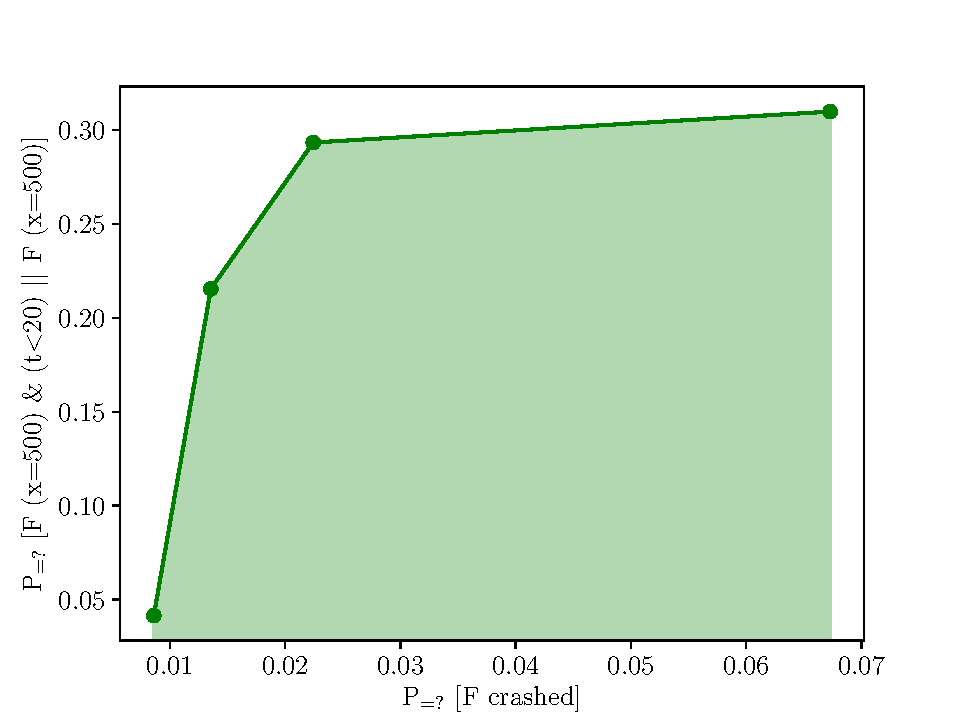
\includegraphics[width=1\textwidth]{test_cases/21_19_70/cond/3_3.pdf}
%  \subcaption{3 (Cautious drivers)}
%\end{subfigure}
%\begin{subfigure}{0.49\textwidth}
%  \centering
%  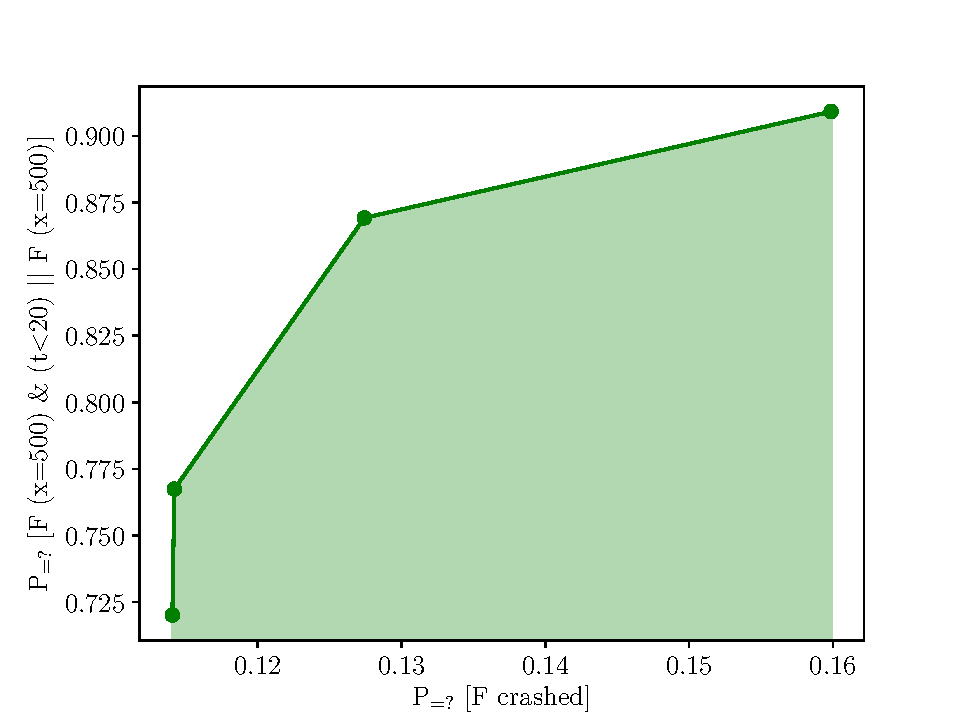
\includegraphics[width=1\textwidth]{test_cases/21_19_70/cond/4_1.pdf}
%  \subcaption{4 (Aggressive drivers)}
%\end{subfigure} 
%\begin{subfigure}{0.49\textwidth}
%  \centering
%  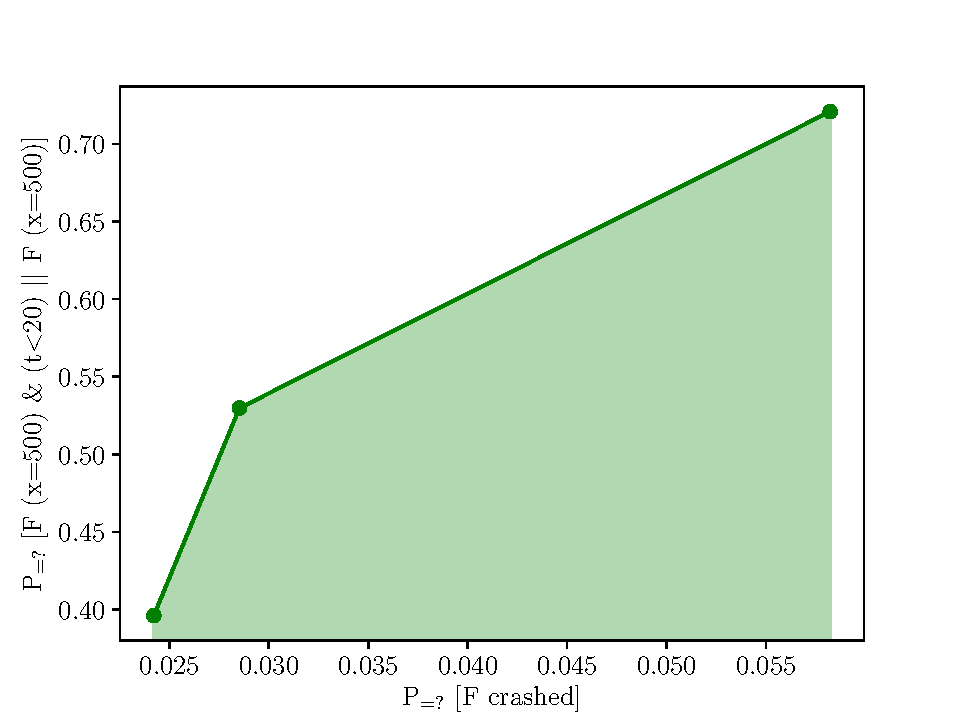
\includegraphics[width=1\textwidth]{test_cases/21_19_70/cond/4_2.pdf}
%  \subcaption{4 (Average drivers)}
%\end{subfigure}
%\begin{subfigure}{0.49\textwidth}
%  \centering
%  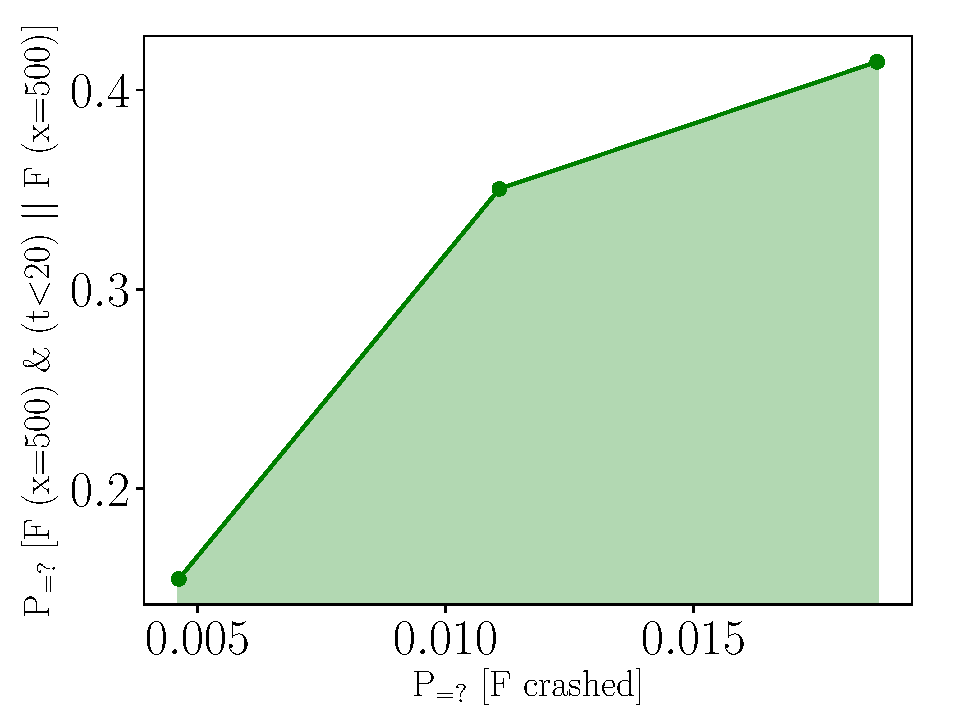
\includegraphics[width=1\textwidth]{test_cases/21_19_70/cond/4_3.pdf}
%  \subcaption{4 (Cautious drivers)}
%\end{subfigure}
%\caption{Pareto curves for the conditional properties, for $T = 20$ (cont.).}
%\end{figure}

%\subsubsection{$v = 30$ m/s, $v_1 = 22$ m/s, $x_{1,0} = 50$ m ($T=19$)}

\begin{figure}[H]
%\vspace{3em}
\centering
\begin{subfigure}{0.32\textwidth}
  \centering
  \includegraphics[width=1\textwidth]{test_cases/30_22_50/uncond/1.pdf}
  \subcaption{(1)}
\end{subfigure}\\
\begin{subfigure}{0.32\textwidth}
  \centering
  \includegraphics[width=1\textwidth]{test_cases/30_22_50/uncond/2_1.pdf}
  \subcaption{(2) - Aggressive drivers}
\end{subfigure} 
\begin{subfigure}{0.32\textwidth}
  \centering
  \includegraphics[width=1\textwidth]{test_cases/30_22_50/uncond/2_2.pdf}
  \subcaption{(2) - Average drivers}
\end{subfigure}
\begin{subfigure}{0.32\textwidth}
  \centering
  \includegraphics[width=1\textwidth]{test_cases/30_22_50/uncond/2_3.pdf}
  \subcaption{(2) - Cautious drivers}
\end{subfigure}
\begin{subfigure}{0.32\textwidth}
  \centering
  \includegraphics[width=1\textwidth]{test_cases/30_22_50/uncond/3_1.pdf}
  \subcaption{(3) - Aggressive drivers}
\end{subfigure}
\begin{subfigure}{0.32\textwidth}
  \centering
  \includegraphics[width=1\textwidth]{test_cases/30_22_50/uncond/3_2.pdf}
  \subcaption{(3) - Average drivers}
\end{subfigure}
\begin{subfigure}{0.32\textwidth}
  \centering
  \includegraphics[width=1\textwidth]{test_cases/30_22_50/uncond/3_3.pdf}
  \subcaption{(3) - Cautious drivers}
\end{subfigure}
\begin{subfigure}{0.32\textwidth}
  \centering
  \includegraphics[width=1\textwidth]{test_cases/30_22_50/uncond/4_1.pdf}
  \subcaption{(4) - Aggressive drivers}
\end{subfigure} 
\begin{subfigure}{0.32\textwidth}
  \centering
  \includegraphics[width=1\textwidth]{test_cases/30_22_50/uncond/4_2.pdf}
  \subcaption{(4) - Average drivers}
\end{subfigure}
\begin{subfigure}{0.32\textwidth}
  \centering
  \includegraphics[width=1\textwidth]{test_cases/30_22_50/uncond/4_3.pdf}
  \subcaption{(4) - Cautious drivers}
\end{subfigure}
\caption{Pareto curves of the unconditional properties for the scenario $v = 30m/s$, $v_1 = 22m/s$, $x_{1,0} = 50m$ and for $T = 19$. The ADAS are represented using the following numbering: (1) decision making-based with fully compliant drivers, (2) decision making-based with partially compliant drivers, (3) decision making with partially compliant drivers + linear acceleration control, and (4) decision making with partially compliant drivers + linear acceleration control + steering control.}
\label{fig:test_case_2_uncond}
\end{figure}

%\begin{figure}[H] \ContinuedFloat
%\centering
%\begin{subfigure}{0.49\textwidth}
%  \centering
%  \includegraphics[width=1\textwidth]{test_cases/30_22_50/uncond/3_3.pdf}
%  \subcaption{3 (Cautious drivers)}
%\end{subfigure}
%\begin{subfigure}{0.49\textwidth}
%  \centering
%  \includegraphics[width=1\textwidth]{test_cases/30_22_50/uncond/4_1.pdf}
%  \subcaption{4 (Aggressive drivers)}
%\end{subfigure} 
%\begin{subfigure}{0.49\textwidth}
%  \centering
%  \includegraphics[width=1\textwidth]{test_cases/30_22_50/uncond/4_2.pdf}
%  \subcaption{4 (Average drivers)}
%\end{subfigure}
%\begin{subfigure}{0.49\textwidth}
%  \centering
%  \includegraphics[width=1\textwidth]{test_cases/30_22_50/uncond/4_3.pdf}
%  \subcaption{4 (Cautious drivers)}
%\end{subfigure}
%\caption{Pareto curves for the unconditional properties, for $T = 19$ (cont.).}
%\label{fig:test_case_2_uncond}
%\end{figure}

\begin{figure}[H]
\vspace{3em}
\centering
\begin{subfigure}{0.32\textwidth}
  \centering
  \includegraphics[width=1\textwidth]{test_cases/30_22_50/cond/1.pdf}
  \subcaption{(1)}
\end{subfigure}\\
\begin{subfigure}{0.32\textwidth}
  \centering
  \includegraphics[width=1\textwidth]{test_cases/30_22_50/cond/2_1.pdf}
  \subcaption{(2) - Aggressive drivers}
\end{subfigure} 
\begin{subfigure}{0.32\textwidth}
  \centering
  \includegraphics[width=1\textwidth]{test_cases/30_22_50/cond/2_2.pdf}
  \subcaption{(2) - Average drivers}
\end{subfigure}
\begin{subfigure}{0.32\textwidth}
  \centering
  \includegraphics[width=1\textwidth]{test_cases/30_22_50/cond/2_3.pdf}
  \subcaption{(2) - Cautious drivers}
\end{subfigure}
\begin{subfigure}{0.32\textwidth}
  \centering
  \includegraphics[width=1\textwidth]{test_cases/30_22_50/cond/3_1.pdf}
  \subcaption{(3) - Aggressive drivers}
\end{subfigure}
\begin{subfigure}{0.32\textwidth}
  \centering
  \includegraphics[width=1\textwidth]{test_cases/30_22_50/cond/3_2.pdf}
  \subcaption{(3) - Average drivers}
\end{subfigure}
\begin{subfigure}{0.32\textwidth}
  \centering
  \includegraphics[width=1\textwidth]{test_cases/30_22_50/cond/3_3.pdf}
  \subcaption{(3) - Cautious drivers}
\end{subfigure}
\begin{subfigure}{0.32\textwidth}
  \centering
  \includegraphics[width=1\textwidth]{test_cases/30_22_50/cond/4_1.pdf}
  \subcaption{(4) - Aggressive drivers}
\end{subfigure} 
\begin{subfigure}{0.32\textwidth}
  \centering
  \includegraphics[width=1\textwidth]{test_cases/30_22_50/cond/4_2.pdf}
  \subcaption{(4) - Average drivers}
\end{subfigure}
\begin{subfigure}{0.32\textwidth}
  \centering
  \includegraphics[width=1\textwidth]{test_cases/30_22_50/cond/4_3.pdf}
  \subcaption{(4) - Cautious drivers}
\end{subfigure}
\caption{Pareto curves of the conditional properties for the scenario $v = 30m/s$, $v_1 = 22m/s$, $x_{1,0} = 50m$ and for $T = 19$. The ADAS are represented using the following numbering: (1) decision making-based with fully compliant drivers, (2) decision making-based with partially compliant drivers, (3) decision making with partially compliant drivers + linear acceleration control, and (4) decision making with partially compliant drivers + linear acceleration control + steering control.}
\label{fig:test_case_2_cond}
\end{figure}

%\begin{figure}[H] \ContinuedFloat
%\centering
%\begin{subfigure}{0.49\textwidth}
%  \centering
%  \includegraphics[width=1\textwidth]{test_cases/30_22_50/cond/3_3.pdf}
%  \subcaption{3 (Cautious drivers)}
%\end{subfigure}
%\begin{subfigure}{0.49\textwidth}
%  \centering
%  \includegraphics[width=1\textwidth]{test_cases/30_22_50/cond/4_1.pdf}
%  \subcaption{4 (Aggressive drivers)}
%\end{subfigure} 
%\begin{subfigure}{0.49\textwidth}
%  \centering
%  \includegraphics[width=1\textwidth]{test_cases/30_22_50/cond/4_2.pdf}
%  \subcaption{4 (Average drivers)}
%\end{subfigure}
%\begin{subfigure}{0.49\textwidth}
%  \centering
%  \includegraphics[width=1\textwidth]{test_cases/30_22_50/cond/4_3.pdf}
%  \subcaption{4 (Cautious drivers)}
%\end{subfigure}
%\caption{Pareto curves for the conditional properties, for $T = 19$ (cont.).}
%\label{fig:test_case_2_cond}
%\end{figure}

\subsection{Overall Comparison}

From the Pareto curves presented, it is noticeable that the best performing ADAS is the first presented, that is, a decision making assistance system with the assumption of fully compliant drivers. This assistance system allows maximum safety (\texttt{P=? [F crashed]} = 0) and efficiency (\texttt{P=? [F (x=500) \& (t<T)]} = 1) for both test cases and respective values of $T$ considered. However, as discussed before, this situation is unrealistic in nature. By adding the partial compliance assumption, the performance drops drastically, leading to fairly high probabilities of crashing in aggressive drivers (minimum of 0.285 for the first test case and 0.294 for the second one) and lower liveness performance as well. By introducing linear acceleration control, safety increases significantly (the probability of crashing is lowered), but the increase of the probability of the liveness property being satisfied is almost negligible in some situations (and it decreases in some cases; e.g. the aggressive drivers in the first test case). In all the cases tested, the introduction of steering control improves, in both cases and for all driver classes, both safety and liveness. Therefore, the assistance system number 4, that is, decision making with partially compliant drivers, active linear acceleration control and active steering control is the best performing system in the two test cases presented (other than number 1, which is based on unrealistic assumptions).

This analysis does not provide a statistical guarantee that this is the best performing ADAS out of the ones tested in the majority of the situations (as this would be too time consuming for the time frame of this dissertation). However, the systems considered are incremental in nature, in the sense that they were built through iteration and by adding more actions to the one immediately before. As such, number 4 was expected for perform better than numbers 2 and 3, simply due to the fact that there were more choices available to it. The two test cases presented corroborate this idea. Therefore, it can be concluded that the assistance system number 4 would be the most complete and better candidate for deployment, and, as such, the in-depth experimental results and discussion presented in Chapter~\ref{sec:results} use this ADAS.

\chapter{Experimental Results}
\label{sec:results}

In this chapter, the performance of the driver assistance system is evaluated by comparing the value of quantitative properties in the human driver model obtained in Chapter~\ref{sec:human_driver} to similar properties in the model of the human driver with the ADAS designed in Chapter~\ref{sec:adas} (decision making with partially compliant drivers and with active linear acceleration and steering control). This is achieved using the various metrics defined throughout the dissertation, through random test cases of initial conditions and further comparison using a randomly generated sample population. After a discussion of the main results, some additional experiments regarding different properties outside the scope of the extensive comparison are presented.

\section{Human driver and ADAS comparison}

\subsection{Safety Results}
\label{sec:res_safety}

As initially described in Chapter~\ref{sec:human_driver}, the safety property for the human driver model can be written as:

\begin{minipage}{\linewidth}
{\vspace{1em}
\begin{lstlisting}
P=? [F crashed]
\end{lstlisting}
}
\end{minipage}

A similar safety property is presented in Chapter~\ref{sec:adas}, adapted for the fact that the model of the human driver and driver assistance system is an MDP instead of a DTMC:

\begin{minipage}{\linewidth}
{\vspace{1em}
\begin{lstlisting}
Pmin=? [F crashed]
\end{lstlisting}
}
\end{minipage}

These properties are directly comparable, as they represent the same quantitative value (this is not the case with the liveness properties). It should be noted that the lower the value of this property, the safer the system is. This means that these properties can be used not only for comparisons between the human driver alone and the full system (human and driver assistance system) for a given scenario, but also for inter-situational comparisons (i.e. with different initial conditions).

A scenario, in both cases, can be uniquely defined as a tuple $(d_{type}, v, v_1, x_{1,0})$, where $d_{type} \in \{1,2,3\}$ is the driver class considered (aggressive, average or cautious, respectively). In practice, this means that, for a road segment of $500m$ and considering $v, v_1 \in \{15,...,34\}$ and $x_{1,0} \in \{1,...,500\}$, there are $20 \times 20 \times 500 \times 3 = 600,000$ different scenarios to consider. Assuming that model checking each of those scenarios for both the human driver and the full system takes 5 minutes each (an assumption which will be challenged in Chapter~\ref{sec:conclusion}), this task would take approximately 2083 days to complete. Given the time frame of this dissertation, this would be infeasible. As such, three other methods where designed as a way to compare both systems: 

\begin{itemize}
	\item \textbf{Main vehicle initial velocity test cases}: for two randomly selected tuples $(v_1, x_{1,0})$, the variation of the value of the safety properties for each driver profile with the variation of $v$ were obtained. This directly compares 20 different scenarios for each driver class. The two tuples were randomly generated as $(v_1, x_{1,0}) = (20, 35)$ and $(v_1, x_{1,0}) = (22, 40)$, and the results are presented in Figures~\ref{fig:plot1} and \ref{fig:plot2}, respectively.
	\item \textbf{Bivariant initial velocity test cases}: for a randomly selected $x_{1,0}$, the variation of the values of the safety properties for each driver profile with the change of $v$ and $v_1$ (within certain ranges; $v \in \{20,...,30\}$ and $v_1\in \{15,...,25\}$) were generated. This directly compares 120 different scenarios for each driver class. The value $x_{1,0} = 50$ was randomly generated for this test case, and the results are presented in Figure~\ref{fig:plot3}.
	\item \textbf{Box plots}: for a randomly generated sample of 100 different initial conditions of $(v, v_1, x_{1,0})$, a box plot which represents the distribution of the values of the safety properties for this sample and for each driver profile was obtained. The results are shown in Figure~\ref{fig:plot6}.
\end{itemize}

\begin{figure}[H]
\centering
\begin{subfigure}{0.75\textwidth}
  \centering
  \includegraphics[width=1\textwidth]{results/safety/plot1_1.pdf}
  \subcaption{Human driver model}
\end{subfigure}
\begin{subfigure}{0.75\textwidth}
  \centering
  \includegraphics[width=1\textwidth]{results/safety/plot1_2.pdf}
  \subcaption{ADAS}
\end{subfigure} 
\caption{Plots of the variation of the value of the safety property with the initial velocity of the main vehicle for the conditions $v_1 = 20m/s$ and $x_{1,0} = 35m$.}
\label{fig:plot1}
\end{figure}

\begin{figure}[H]
\centering
\begin{subfigure}{0.75\textwidth}
  \centering
  \includegraphics[width=1\textwidth]{results/safety/plot2_1.pdf}
  \subcaption{Human driver model}
\end{subfigure}
\begin{subfigure}{0.75\textwidth}
  \centering
  \includegraphics[width=1\textwidth]{results/safety/plot2_2.pdf}
  \subcaption{ADAS}
\end{subfigure} 
\caption{Plots of the variation of the value of the safety property with the initial velocity of the main vehicle for the conditions $v_1 = 22m/s$ and $x_{1,0} = 40m$.}
\label{fig:plot2}
\end{figure}

\begin{figure}[H]
\centering
\begin{subfigure}{0.5\textwidth}
  \centering
  \includegraphics[width=1\textwidth]{results/safety/plot3_aggressive.pdf}
  \subcaption{Aggressive drivers}
\end{subfigure}
\begin{subfigure}{0.5\textwidth}
  \centering
  \includegraphics[width=1\textwidth]{results/safety/plot3_average.pdf}
  \subcaption{Average drivers}
\end{subfigure} 
\begin{subfigure}{0.5\textwidth}
  \centering
  \includegraphics[width=1\textwidth]{results/safety/plot3_cautious.pdf}
  \subcaption{Cautious drivers}
\end{subfigure} 
\caption{Variation of the value of the safety properties with the initial velocities of both vehicles for $x_{1,0} = 50m$.}
\label{fig:plot3}
\end{figure}

\begin{figure}[H]
\centering
\begin{subfigure}{0.75\textwidth}
  \centering
  \includegraphics[width=1\textwidth]{results/safety/plot6_1.pdf}
  \subcaption{Human driver model}
\end{subfigure}
\begin{subfigure}{0.75\textwidth}
  \centering
  \includegraphics[width=1\textwidth]{results/safety/plot6_2.pdf}
  \subcaption{ADAS}
\end{subfigure} 
\caption{Box plot of the value of the safety properties for a randomly sampled population of 100 different initial conditions (equal in both cases).}
\label{fig:plot6}
\end{figure}

\subsection{Liveness Results}
\label{sec:res_liveness}

As introduced in Chapter~\ref{sec:human_driver}, there are multiple liveness properties that can be considered when evaluating the human driver model. However, the most appropriate ones for inter-situational comparisons are the conditional properties of the type:

\begin{minipage}{\linewidth}
{\vspace{1em}
\begin{lstlisting}
P=? [F (x=length) & (t<T) || F (x=length)]
\end{lstlisting}
}
\end{minipage}

for a given constant $T$.

In the case of the full system (human driver and ADAS), the model becomes an MDP and, as mentioned in Chapter~\ref{sec:background}, conditional properties are not so easily calculated in MDPs due to the existence of multiple adversaries. Despite this, it is possible to reason over lower bounds of these types of properties under the conditions of Proposition~\ref{pro:cond_props}. For the PCTL formulas $\varphi_1 = $\texttt{ F (x=length) \& (t<T)} and $\varphi_2 = $\texttt{ F (x=length)}, it is trivial that for any path $\pi \in Paths(s)$: $\pi \models \varphi_1 \Rightarrow \pi \models \varphi_2$. Furthermore, it can also be assumed that for:

\begin{equation}
	\sigma' \in \arg\sup_{\sigma \in Adv} P^{\sigma}_s (\varphi_1 \bigmid \varphi_2)
\end{equation}

it is true that:

\begin{equation}
	P^{\sigma'}_s (\varphi_1) = p_{\max, s} (\varphi_1)
\end{equation}

since intuitively the interest is in adversaries which maximise the conditional property through the maximisation of the probability of eventually reaching \texttt{(x=length) \& (t<T)} (as this is the comparable case in the human driver model). Thus, under the conditions of Proposition~\ref{pro:cond_props}, it is possible to write:

\begin{equation}
	p_{\max, s} (\text{\texttt{F (x=length) \& (t<T)}} \bigmid \text{\texttt{F (x=length)}}) \geq \frac{p_{\max, s} (\text{\texttt{F (x=length) \& (t<T)}})}{p_{\max, s} (\text{\texttt{F (x=length)}})}
\end{equation}

Therefore, a lower bound on the conditional probability, $\zeta$, can be obtained using the quantitative properties:

\begin{equation}
	\zeta = \frac{\text{\texttt{Pmax=? [F (x=length) \& (t<T)]}}}{\text{\texttt{Pmax=? [F (x=length)]}}}
\end{equation}

At this point it should also be noted that (as described in Section~\ref{sec:multi_obj_metrics}):

\begin{equation}
	p_{\max,s} (\text{\texttt{F x=length}}) = 1 - p_{\min,s} (\text{\texttt{F crashed}})
\end{equation}

so long as $p_{\max, s} (\text{\texttt{F (crashed | x = length)}}) = p_{\min, s} (\text{\texttt{F (crashed | x = length)}}) = 1$ (completeness property for the MDP). Therefore, $\zeta$ can be re-written as:

\begin{equation}
	\zeta = \frac{\text{\texttt{Pmax=? [F (x=length) \& (t<T)]}}}{1 - \text{\texttt{Pmin=? [F crashed]}}}
\end{equation}

As was the case with the safety properties, model checking the entire space of possible initial conditions would be infeasible given the time frame of this dissertation. Similarly, two methods were designed to compare both systems at the liveness level:

\begin{itemize}
	\item \textbf{Temporal variation of liveness}: for two randomly selected tuples $(v, v_1, x_{1,0})$, the value of all the pertinent liveness properties ($T \in \{16,...,28\}$) was obtained. The two tuples were randomly generated as $(v, v_1, x_{1,0}) = (21, 19, 70)$ and $(v, v_1, x_{1,0}) = (26, 22, 46)$, and the results are presented in Figures~\ref{fig:plot4} and \ref{fig:plot5}, respectively.
	\item \textbf{Box plots}: for a randomly generated sample of 100 different initial conditions of $(v, v_1, x_{1,0})$, obtain box plot which represents the distribution of the values of two liveness properties using appropriate values of $T$ (given the sample) for this sample and for each driver profile. After the sample was generated, it was determined that $T=21$ and $T=22$ were representative values (in the sense that they are great enough to avoid a significant portion of the values of both properties being 0, and not so large that a significant portion of the values for all scenarios are 1; these situations would make it impossible to compare the human and the full system). The results are presented in Figures~\ref{fig:plot7} and \ref{fig:plot8} for $T=21$ and $T=22$, respectively.
\end{itemize}

\begin{figure}[H]
\centering
\begin{subfigure}{0.75\textwidth}
  \centering
  \includegraphics[width=1\textwidth]{results/liveness/plot4_1.pdf}
  \subcaption{Human driver model}
\end{subfigure}
\begin{subfigure}{0.75\textwidth}
  \centering
  \includegraphics[width=1\textwidth]{results/liveness/plot4_2.pdf}
  \subcaption{ADAS}
\end{subfigure} 
\caption{Plots of the variation of the value of the liveness properties with the value of $T$ (in $s$) for the initial conditions $v = 21m/s$, $v_1 = 19m/s$ and $x_{1,0} = 70m$.}
\label{fig:plot4}
\end{figure}

\begin{figure}[H]
\centering
\begin{subfigure}{0.75\textwidth}
  \centering
  \includegraphics[width=1\textwidth]{results/liveness/plot5_1.pdf}
  \subcaption{Human driver model}
\end{subfigure}
\begin{subfigure}{0.75\textwidth}
  \centering
  \includegraphics[width=1\textwidth]{results/liveness/plot5_2.pdf}
  \subcaption{ADAS}
\end{subfigure} 
\caption{Plots of the variation of the value of the liveness properties with the value of $T$ (in $s$) for the initial conditions $v = 26m/s$, $v_1 = 22m/s$ and $x_{1,0} = 46m$.}
\label{fig:plot5}
\end{figure}

\begin{figure}[H]
\centering
\begin{subfigure}{0.75\textwidth}
  \centering
  \includegraphics[width=1\textwidth]{results/liveness/plot7_1.pdf}
  \subcaption{Human driver model}
\end{subfigure}
\begin{subfigure}{0.75\textwidth}
  \centering
  \includegraphics[width=1\textwidth]{results/liveness/plot7_2.pdf}
  \subcaption{ADAS}
\end{subfigure} 
\caption{Box plot of the value of the liveness properties for $T = 21s$ for a randomly sampled population of 50 different initial conditions (equal in both cases).}
\label{fig:plot7}
\end{figure}

\begin{figure}[H]
\centering
\begin{subfigure}{0.75\textwidth}
  \centering
  \includegraphics[width=1\textwidth]{results/liveness/plot8_1.pdf}
  \subcaption{Human driver model}
\end{subfigure}
\begin{subfigure}{0.75\textwidth}
  \centering
  \includegraphics[width=1\textwidth]{results/liveness/plot8_2.pdf}
  \subcaption{ADAS}
\end{subfigure} 
\caption{Box plot of the value of the liveness properties for $T = 22s$ for a randomly sampled population of 50 different initial conditions (equal in both cases).}
\label{fig:plot8}
\end{figure}

\subsection{Discussion}

The discussion of the results presented in Sections~\ref{sec:res_safety} and \ref{sec:res_liveness} is threefold in nature. Firstly, the comparison between the different driver classes within each of the individual systems (i.e. human driver model and the human and ADAS system) is presented. Secondly, the results of the experiments of the human driver alone and the full system in both safety and liveness are discussed and compared (within the same driver profile). Finally, an overall discussion is presented on the extent of the validity of such comparisons through the drawbacks of the metrics used.

With respect to the individual driver classes presented in both the human driver model and the human and ADAS system, the results overwhelmingly support the initial idea that aggressive drivers perform the worse in terms of the safety metrics, followed by average drivers and finally cautious ones. While this is observable in the individual test cases (Figures~\ref{fig:plot1} and \ref{fig:plot2}), Figure~\ref{fig:plot6} firmly supports this conclusion within both systems. In terms of liveness, the reverse is true, with aggressive drivers outperforming average drivers who in turn outperform cautious drivers. Once more, while individual test cases support this result (Figures~\ref{fig:plot4} and \ref{fig:plot5}), Figures~\ref{fig:plot7} and \ref{fig:plot8} emphatically reinforce it. Intuitively, this is what was expected from the construction of the human driver model, and it is still noticeable even using the ADAS designed.

In terms of the comparison between the human driver model and the driver with the ADAS system, it becomes necessary to interpret the plots while considering the differences in the metrics used. 

In the safety evaluation, as mentioned in Section~\ref{sec:res_safety}, the results are directly comparable as the metrics are the equivalent of one another for the representation of the models of both systems (i.e. a DTMC for the human driver model and an MDP for the human and ADAS system). The most useful comparison in terms of the test cases in this metric is presented in Figure~\ref{fig:plot3}, as the 3D plots are divided into the three categories of drivers considered. It is observable that the introduction of the ADAS increases safety for all situations considered in this test case (i.e. reduces the value of the safety property). From the more general overview seen in Figures~\ref{fig:plot7} and \ref{fig:plot8}, the same conclusion is drawn for each driver class, with the $25\%$, $50\%$ (median) and $75\%$ quartiles being lower for the system with the ADAS than those for the human driver alone. 

With respect to liveness, the comparison needs to be carefully drawn, as the conditional property in the human driver model alone (DTMC) is not the equivalent of the metric chosen for liveness in the human and ADAS system (MDP). However, $\zeta$ is proven to be the lower bound of the conditional property in the human and ADAS system under the conditions presented in Section~\ref{sec:res_liveness}. From Figures~\ref{fig:plot4} and \ref{fig:plot5}, it can be observed that, for each $T$, the values of $\zeta$ are always greater or equal than those of the conditional property of the human driver model. The same result can be seen in Figures~\ref{fig:plot7} and \ref{fig:plot8} for $T=21$ and $T=22$, respectively, for the $25\%$ and $75\%$ quartiles. Given that $\zeta$ is the lower bound of the maximal conditional property, it can be concluded that the system with the ADAS outperforms the human driver alone in this metric. 

Despite the results pointing to the improvements in terms of the safety and liveness properties the ADAS designed brings, they should be taken with care, as there are drawbacks in the metrics used. 

The first drawback has to do with the fact that the comparison in the human and ADAS deals with minimal and maximal properties due to the existence of adversaries in MDPs. Thus, the fact that the safety property is lower in this case than in the human driver model and the liveness properties are higher, does not mean that there is a feasible strategy where both safety and liveness are optimal and outperform the human driver (there might be a trade-off). This is not the case with the human driver model, where it is known that both quantitative properties are satisfied simultaneously. In order to evaluate this feasibility properly, Pareto curves should be generated for each individual scenario and it should be seen whether there exists a Pareto point where both values outperform the human driver. This analysis is time consuming with the tools currently available (i.e. PRISM and Storm) and was therefore infeasible in the time frame of this dissertation. 

An additional drawback in terms of the liveness properties in the full system (i.e. human driver and ADAS system) case is that these are defined as lower bounds which are not proven to be tight. In fact, in Figure~\ref{fig:plot8}, while the $25\%$ and $75\%$ quartiles appear to be higher in the case of the full system than the human driver model, this is not the case with the median, which is at similar values (or even lower for the class of cautious drivers). From the rest of the data, it would appear that this value might be the result of the fact that the lower bound is not tight and might be underestimating the value of the maximal conditional property for the sample population used. However, this is not certain, and it might also be that the full system is outperformed, in terms of the liveness properties, by the human driver in certain conditions. The use of the unconditional liveness properties here would be meaningless, as it would incur in the safety bias first presented in Section~\ref{sec:live_props}. A solution to this problem would be to develop the tools to model check conditional properties in MDPs, however, this was outside the scope of this dissertation and would be highly time consuming.

\section{Additional Experiments}
\label{sec:add_exp}

While outside the scope of the main goal of the dissertation of evaluating safety and liveness, additional properties can be used to synthesise strategies for the ADAS which enforce other types of behaviours. 

\subsection{Left Lane Penalising}

When a driver attempts an overtake of the lead vehicle, it should do so by performing two lane changes, one from the current lane to the one immediately to the left, and another one to return to the original lane after it has passed the lead vehicle. The manoeuvre should be performed safely, yet as quickly as possible \cite{carr}. With this in mind, properties can be specified to assert such a regulation to the ADAS to guarantee compliance.

In particular, the property should penalise the usage of the left lane ($lane = 2$). For this purpose, the following reward structure was designed:

\begin{minipage}{\linewidth}
{\vspace{1em}
\begin{lstlisting}
rewards
	[] lane = 1: 0;
	[] lane = 2: 1;
endrewards
\end{lstlisting}
}
\end{minipage}

And the property:

\begin{minipage}{\linewidth}
{\vspace{1em}
\begin{lstlisting}
Rmin=? [C]
\end{lstlisting}
}
\end{minipage}

minimises the cumulative value of this reward, and, therefore, the time spent in the left lane. Thus, the following multi-objective property is introduced:

\begin{minipage}{\linewidth}
{\vspace{1em}
\begin{lstlisting}
multi(Pmin=? [F crashed], Rmin=? [C])
\end{lstlisting}
}
\end{minipage}

To exemplify the use of this reward structure and property, the scenario $(d_{type}, v, v_1, x_{1,0}) = (1, 30, 22, 50)$ (an aggressive driver with an initial speed of $30m/s$ and a lead vehicle at a distance of $50m$ going at $22m/s$) is considered. It should also be noted that the length of the road segment considered in this case was $400m$. By verifying this property, the Pareto curve obtained is presented in Figure~\ref{fig:lane_penalising_pareto}

\begin{figure}[H]
\centering
\includegraphics[width=0.75\textwidth]{results/additional/pareto.pdf}
\caption{Pareto curve for the model checking of the lane penalising property.}
\label{fig:lane_penalising_pareto}
\end{figure}

Observing this curve, it is possible to conclude that it is feasible to have \texttt{R<=1.8 [C]}, and thus the following property:

\begin{minipage}{\linewidth}
{\vspace{1em}
\begin{lstlisting}
multi(Pmin=? [F crashed], R<=1.8 [C])
\end{lstlisting}
}
\end{minipage}

yields an adversary which can be used to generate a sample path in the model. Similarly to what is presented in Section~\ref{sec:simulator}, a simulator was created to allow for the visualisation of a path in the model (the code for which is shown in Appendix~\ref{sec:strat_synth_and_sym}). The results of the simulation are presented in Figure~\ref{fig:lane_penalising_sim}.

\begin{figure}[H]
\centering
\begin{subfigure}{0.75\textwidth}
  \centering
  \includegraphics[width=1\textwidth]{results/additional/snap_1.png}
\end{subfigure}\\ \vspace{2px}
\begin{subfigure}{0.75\textwidth}
  \centering
  \includegraphics[width=1\linewidth]{results/additional/snap_2.png}
\end{subfigure} \\ \vspace{2px}
\begin{subfigure}{0.75\textwidth}
  \centering
  \includegraphics[width=1\linewidth]{results/additional/snap_3.png}
\end{subfigure} \\ \vspace{2px}
\begin{subfigure}{0.75\textwidth}
  \centering
  \includegraphics[width=1\linewidth]{results/additional/snap_4.png}
\end{subfigure} \\ \vspace{2px}
\begin{subfigure}{0.75\textwidth}
  \centering
  \includegraphics[width=1\linewidth]{results/additional/snap_5.png}
\end{subfigure} \\ \vspace{2px}
\begin{subfigure}{0.75\textwidth}
  \centering
  \includegraphics[width=1\linewidth]{results/additional/snap_6.png}
\end{subfigure}
\caption{Snapshots of the simulator for one of the paths of the model.}
\label{fig:lane_penalising_sim}
\end{figure}

As observed, minimal time is spent in the left lane, with the main vehicle returning to the right lane as soon as it passes the lead vehicle.

%\textbf{Three-objective Properties}
%
%In order to guarantee more than only safety and liveness in the model, an alternative to this would be to include multi-objective properties with more than 2 objectives. Such a property would have the format of the one below:
%
%\begin{minipage}{\linewidth}
%{\vspace{1em}
%\begin{lstlisting}
%multi(Pmin=? [F crashed], Pmax=? [F (x=length) & (t<T)], Rmin=? [C])
%\end{lstlisting}
%}
%\end{minipage}
%
%for a given constant $T$ and well defined reward structure. However, neither PRISM nor Storm allow for the model checking of these properties and the generation of the 3D Pareto curve they would entail.

\subsection{Unsafe by Construction}

Until this point, the assumption has been that the goal of the assistance system was to enforce safety and liveness. However, assume a bad actor has access to the model and the deployment process used in the vehicle. In such a case, it becomes important to evaluate the extent of the damage that such an actor could do. Take the same scenario as above, $(d_{type}, v, v_1, x_{1,0}) = (1, 30, 22, 50)$. Let's also assume that the bad actor wants the accident to happen after the the driver has driven between the $100$ and $200m$. The following property can be considered:

\begin{minipage}{\linewidth}
{\vspace{1em}
\begin{lstlisting}
multi(Pmax=? [F crashed], Pmax=? [x <= 100 U (x>100 & x<=200)])
\end{lstlisting}
}
\end{minipage}

which, when model checked, generates a Pareto curve of the trade-off between maximising the probability of crashing and the probability of reaching at least $100m$ and at most $200m$. The Pareto curve generated is presented in Figure~\ref{fig:unsafe_pareto}.

\begin{figure}[H]
\centering
\includegraphics[width=0.75\textwidth]{results/additional/pareto_crashed.pdf}
\caption{Pareto curve for the model checking of the unsafe driving property.}
\label{fig:unsafe_pareto}
\end{figure}

By observing the Pareto curve, the following property can be devised:

\begin{minipage}{\linewidth}
{\vspace{1em}
\begin{lstlisting}
multi(Pmax=? [F crashed], P>=0.5 [x <= 100 U (x>100 & x<=200)])
\end{lstlisting}
}
\end{minipage}

This property maximises the probability of crashing, while requiring the vehicle to drive for at least $100m$ and at most $200m$ with probability at least 0.5 before the crash happens. By model checking this property, the maximum value of \texttt{P=? [F crashed]} comes out to be 0.5326, and the adversary obtained permits the generation of paths such as the one presented in the simulator frames in Figure~\ref{fig:unsafe_sim}. It should be noted that the value of \texttt{P=? [F crashed]} in the human driver model is 0.3935, and thus the bad actor has successfully increased the probability of crashing. 

\vspace{1em}
\begin{figure}[H]
\centering
\begin{subfigure}{0.75\textwidth}
  \centering
  \includegraphics[width=1\textwidth]{results/additional/crash_1.png}
\end{subfigure}\\ \vspace{2px}
\begin{subfigure}{0.75\textwidth}
  \centering
  \includegraphics[width=1\linewidth]{results/additional/crash_2.png}
\end{subfigure} \\ \vspace{2px}
\begin{subfigure}{0.75\textwidth}
  \centering
  \includegraphics[width=1\linewidth]{results/additional/crash_3.png}
\end{subfigure}
\caption{Snapshots of the simulator for one of the paths of the model.}
\label{fig:unsafe_sim}
\end{figure}












\chapter{Conclusions and Future Work}
\label{sec:conclusion}

This dissertation attempted to demonstrate the benefits of using model checking and synthesis to generate correct-by-construction driver assistance systems through an application using a cognitive architecture. This required a model of a human driver in a cognitive architecture to be implemented in PRISM's modelling language. Since Salvucci established his driver model in ACT-R in \cite{salvucci_1}, this dissertation focused on the abstraction process to convert the integrated continuous model into a discrete-time Markov chain. This was done using efficient simulation techniques, which allowed the generated models to be relatively small in terms of state space and transitions. Afterwards, several designs were considered in terms of the capabilities and placement of the driver assistance system within the model. These options ranged from suggestions at the decision making level to correcting linear or steering acceleration. They were evaluated carefully, and the best performing one was then more extensively compared to the human driver model previously obtained. The results showed a significant performance increase (in terms of the metrics used) by the introduction of the driver assistance system.

Most of the expected contributions were achieved. The modelling of a complex scenario (a 2-lane highway and the interactions that arise with various profiles of drivers e.g. follow, crash or overtake another vehicle) through the abstraction of Salvucci's human driver model presented in \cite{salvucci_1} was achieved through the use of efficient simulation techniques and automation of the model writing which lead to compact models (e.g. in \cite{lam}, Lam considers a one way road with at most $270m$, and \cite{games} considers similarly simple scenarios through its model assumptions). For a road length of $500m$, none of the initial conditions considered had a model with more than 700 states, an achievement given the original complexity of the scenario and the constraints of the ACT-R architecture. The establishment of insightful metrics in terms of safety and liveness and their application to multi-objective synthesis of possible ADAS was another central achievement of the dissertation (e.g. in \cite{lam}, only single-objective safety centric metrics are considered). Furthermore, it should be noted that, as shown in Chapter~\ref{sec:results}, the final models (human driver and ADAS) obtained were also manageable in terms of size - with none exceeding 1 million states - an accomplishment as it shows the methodology's flexibility towards even more complex models. These two main achievements combined pave the way for the establishment of a general framework which can be used to tackle similar driving situations (e.g. intersections, multilane highways with more vehicles or urban driving), another aim of the dissertation. 

Despite the achievements and the contributions of this work, there are several limitations to the methodology introduced. The first limitation is the building time of the models. While the models built have a relatively small state space, the building time is quite high for both the human driver model and the full system (human and ADAS), as shown in Section~\ref{sec:res_state}. This is mostly due to the simulation and the tables which result out of this process. While these reduce the state space of the final model, they make the model description quite big (particularly compared to other similarly sized models found in \cite{lam, games}). The model checking tool, in turn, then takes quite some time to process the description files, leading to high building times for the models. Despite this, the time can be reduced by the selection of the right tool and engine (e.g. the sparse engine in Storm outperforms all the engines PRISM supports for the human driver model, but PRISM's hybrid engine outperforms all of Storm's engines in the full model). 

A second limitation has to do with the tools available. As the reader might have noticed, the models presented in Section~\ref{sec:add_exp} were built considering a road segment of $400m$ instead of the $500m$ assumed throughout the rest of the dissertation. This came from the fact that the adversary generation options in PRISM (\texttt{-adv} or \texttt{-advmdp}) make use of the LP engine which, as of right now, is not capable of solving a problem as big as this would have been for the length of $500m$ (despite the MDP having under $500,000$ states). Another limitation of the methodology has to do with the lack of support for the model checking of conditional properties in MDPs in both PRISM and Storm (despite the latter being able to verify them in DTMCs). While PRISM does not support the generation of Pareto curves for more than two objectives, PRISM-games - an extension of PRISM to stochastic multi-player games \cite{prism_games} - does so. However, this tool does not use a symbolic representation of the model and, as such, is quite limited in terms of the size of the models it supports.

The final limitation presented is related to the underlying assumptions made and the usefulness of the driver assistance systems generated. There were quite some assumptions made throughout the dissertation which are not necessarily true. While the control laws that Salvucci presents in \cite{salvucci_1} are the result of corrections made to his original laws presented in \cite{salvucci_0} through the use of real data he collected, most of the assumptions used in this dissertations (e.g. driver profiles) are not. As such, while it is still possible to compare between situations and discuss the advantages of the driver assistance system, it is questionable to what degree the ADAS synthesised in the course of this dissertation are actually accurate and useful. 

In the future, the model description might be reduced through pre-computation and elimination of the guards that are never satisfied within the modules, which make up a significant portion of the file. Furthermore, a data driven approach should be followed to validate the results obtained and correct the assumptions made about the drivers. Once the models are accurate according to the real world data, it is possible to deploy the solutions obtained.

Extensions of this work might include implementations of similar driving situations using the ideas presented in terms of abstraction and driver assistance in order to validate the approach. A framework to formalise and generalise the process of obtaining the driver assistance systems can also be the focus of future research in this area. 










%now enable appendix numbering format and include any appendices
\appendix
\chapter{Code for Human Driver Modelling}

\section{ACT-R Implementation (Matlab)}

\subsection{Main Loop}

Lorem ipsum dolor sit amet, consectetur adipiscing elit. Pellentesque accumsan magna eu metus congue, vitae tristique enim commodo. Aliquam consectetur porttitor nisl, eget pulvinar quam venenatis eget. Aliquam erat volutpat. Nullam at ipsum at felis tincidunt consequat non sed mi. Morbi placerat iaculis dapibus. Aliquam non risus ac urna interdum pretium. Donec maximus, massa vitae suscipit congue, ligula purus sagittis magna, vitae interdum enim dui sed felis. Curabitur mollis eleifend diam a varius. Vivamus eu porttitor lorem. Mauris sagittis ultrices ligula, a euismod mi efficitur a. Aenean molestie sapien a nibh suscipit, nec venenatis urna varius. Sed eu ex id lacus tincidunt ultricies. Aenean quam massa, dignissim ac suscipit posuere, varius sit amet turpis. Nunc semper turpis ullamcorper elit venenatis, in molestie nulla fermentum.

\subsection{Control Module}

Lorem ipsum dolor sit amet, consectetur adipiscing elit. Pellentesque accumsan magna eu metus congue, vitae tristique enim commodo. Aliquam consectetur porttitor nisl, eget pulvinar quam venenatis eget. Aliquam erat volutpat. Nullam at ipsum at felis tincidunt consequat non sed mi. Morbi placerat iaculis dapibus. Aliquam non risus ac urna interdum pretium. Donec maximus, massa vitae suscipit congue, ligula purus sagittis magna, vitae interdum enim dui sed felis. Curabitur mollis eleifend diam a varius. Vivamus eu porttitor lorem. Mauris sagittis ultrices ligula, a euismod mi efficitur a. Aenean molestie sapien a nibh suscipit, nec venenatis urna varius. Sed eu ex id lacus tincidunt ultricies. Aenean quam massa, dignissim ac suscipit posuere, varius sit amet turpis. Nunc semper turpis ullamcorper elit venenatis, in molestie nulla fermentum.

\subsection{Decision Making Module}

Lorem ipsum dolor sit amet, consectetur adipiscing elit. Pellentesque accumsan magna eu metus congue, vitae tristique enim commodo. Aliquam consectetur porttitor nisl, eget pulvinar quam venenatis eget. Aliquam erat volutpat. Nullam at ipsum at felis tincidunt consequat non sed mi. Morbi placerat iaculis dapibus. Aliquam non risus ac urna interdum pretium. Donec maximus, massa vitae suscipit congue, ligula purus sagittis magna, vitae interdum enim dui sed felis. Curabitur mollis eleifend diam a varius. Vivamus eu porttitor lorem. Mauris sagittis ultrices ligula, a euismod mi efficitur a. Aenean molestie sapien a nibh suscipit, nec venenatis urna varius. Sed eu ex id lacus tincidunt ultricies. Aenean quam massa, dignissim ac suscipit posuere, varius sit amet turpis. Nunc semper turpis ullamcorper elit venenatis, in molestie nulla fermentum.

\subsection{Monitoring Module}

Lorem ipsum dolor sit amet, consectetur adipiscing elit. Pellentesque accumsan magna eu metus congue, vitae tristique enim commodo. Aliquam consectetur porttitor nisl, eget pulvinar quam venenatis eget. Aliquam erat volutpat. Nullam at ipsum at felis tincidunt consequat non sed mi. Morbi placerat iaculis dapibus. Aliquam non risus ac urna interdum pretium. Donec maximus, massa vitae suscipit congue, ligula purus sagittis magna, vitae interdum enim dui sed felis. Curabitur mollis eleifend diam a varius. Vivamus eu porttitor lorem. Mauris sagittis ultrices ligula, a euismod mi efficitur a. Aenean molestie sapien a nibh suscipit, nec venenatis urna varius. Sed eu ex id lacus tincidunt ultricies. Aenean quam massa, dignissim ac suscipit posuere, varius sit amet turpis. Nunc semper turpis ullamcorper elit venenatis, in molestie nulla fermentum.

\section{Control Abstraction (Matlab)}

Lorem ipsum dolor sit amet, consectetur adipiscing elit. Pellentesque accumsan magna eu metus congue, vitae tristique enim commodo. Aliquam consectetur porttitor nisl, eget pulvinar quam venenatis eget. Aliquam erat volutpat. Nullam at ipsum at felis tincidunt consequat non sed mi. Morbi placerat iaculis dapibus. Aliquam non risus ac urna interdum pretium. Donec maximus, massa vitae suscipit congue, ligula purus sagittis magna, vitae interdum enim dui sed felis. Curabitur mollis eleifend diam a varius. Vivamus eu porttitor lorem. Mauris sagittis ultrices ligula, a euismod mi efficitur a. Aenean molestie sapien a nibh suscipit, nec venenatis urna varius. Sed eu ex id lacus tincidunt ultricies. Aenean quam massa, dignissim ac suscipit posuere, varius sit amet turpis. Nunc semper turpis ullamcorper elit venenatis, in molestie nulla fermentum.

\section{Decision Making and Monitoring Abstraction (Matlab)}

Lorem ipsum dolor sit amet, consectetur adipiscing elit. Pellentesque accumsan magna eu metus congue, vitae tristique enim commodo. Aliquam consectetur porttitor nisl, eget pulvinar quam venenatis eget. Aliquam erat volutpat. Nullam at ipsum at felis tincidunt consequat non sed mi. Morbi placerat iaculis dapibus. Aliquam non risus ac urna interdum pretium. Donec maximus, massa vitae suscipit congue, ligula purus sagittis magna, vitae interdum enim dui sed felis. Curabitur mollis eleifend diam a varius. Vivamus eu porttitor lorem. Mauris sagittis ultrices ligula, a euismod mi efficitur a. Aenean molestie sapien a nibh suscipit, nec venenatis urna varius. Sed eu ex id lacus tincidunt ultricies. Aenean quam massa, dignissim ac suscipit posuere, varius sit amet turpis. Nunc semper turpis ullamcorper elit venenatis, in molestie nulla fermentum.

\section{Probabilistic Two Module Model Generator (Python)}

Lorem ipsum dolor sit amet, consectetur adipiscing elit. Pellentesque accumsan magna eu metus congue, vitae tristique enim commodo. Aliquam consectetur porttitor nisl, eget pulvinar quam venenatis eget. Aliquam erat volutpat. Nullam at ipsum at felis tincidunt consequat non sed mi. Morbi placerat iaculis dapibus. Aliquam non risus ac urna interdum pretium. Donec maximus, massa vitae suscipit congue, ligula purus sagittis magna, vitae interdum enim dui sed felis. Curabitur mollis eleifend diam a varius. Vivamus eu porttitor lorem. Mauris sagittis ultrices ligula, a euismod mi efficitur a. Aenean molestie sapien a nibh suscipit, nec venenatis urna varius. Sed eu ex id lacus tincidunt ultricies. Aenean quam massa, dignissim ac suscipit posuere, varius sit amet turpis. Nunc semper turpis ullamcorper elit venenatis, in molestie nulla fermentum.

\section{Prism Automatic Model Checker (Python)}

Lorem ipsum dolor sit amet, consectetur adipiscing elit. Pellentesque accumsan magna eu metus congue, vitae tristique enim commodo. Aliquam consectetur porttitor nisl, eget pulvinar quam venenatis eget. Aliquam erat volutpat. Nullam at ipsum at felis tincidunt consequat non sed mi. Morbi placerat iaculis dapibus. Aliquam non risus ac urna interdum pretium. Donec maximus, massa vitae suscipit congue, ligula purus sagittis magna, vitae interdum enim dui sed felis. Curabitur mollis eleifend diam a varius. Vivamus eu porttitor lorem. Mauris sagittis ultrices ligula, a euismod mi efficitur a. Aenean molestie sapien a nibh suscipit, nec venenatis urna varius. Sed eu ex id lacus tincidunt ultricies. Aenean quam massa, dignissim ac suscipit posuere, varius sit amet turpis. Nunc semper turpis ullamcorper elit venenatis, in molestie nulla fermentum.

\section{Storm Automatic Model Checker (Python)}

Lorem ipsum dolor sit amet, consectetur adipiscing elit. Pellentesque accumsan magna eu metus congue, vitae tristique enim commodo. Aliquam consectetur porttitor nisl, eget pulvinar quam venenatis eget. Aliquam erat volutpat. Nullam at ipsum at felis tincidunt consequat non sed mi. Morbi placerat iaculis dapibus. Aliquam non risus ac urna interdum pretium. Donec maximus, massa vitae suscipit congue, ligula purus sagittis magna, vitae interdum enim dui sed felis. Curabitur mollis eleifend diam a varius. Vivamus eu porttitor lorem. Mauris sagittis ultrices ligula, a euismod mi efficitur a. Aenean molestie sapien a nibh suscipit, nec venenatis urna varius. Sed eu ex id lacus tincidunt ultricies. Aenean quam massa, dignissim ac suscipit posuere, varius sit amet turpis. Nunc semper turpis ullamcorper elit venenatis, in molestie nulla fermentum.

\section{Simulator (Python)}

Lorem ipsum dolor sit amet, consectetur adipiscing elit. Pellentesque accumsan magna eu metus congue, vitae tristique enim commodo. Aliquam consectetur porttitor nisl, eget pulvinar quam venenatis eget. Aliquam erat volutpat. Nullam at ipsum at felis tincidunt consequat non sed mi. Morbi placerat iaculis dapibus. Aliquam non risus ac urna interdum pretium. Donec maximus, massa vitae suscipit congue, ligula purus sagittis magna, vitae interdum enim dui sed felis. Curabitur mollis eleifend diam a varius. Vivamus eu porttitor lorem. Mauris sagittis ultrices ligula, a euismod mi efficitur a. Aenean molestie sapien a nibh suscipit, nec venenatis urna varius. Sed eu ex id lacus tincidunt ultricies. Aenean quam massa, dignissim ac suscipit posuere, varius sit amet turpis. Nunc semper turpis ullamcorper elit venenatis, in molestie nulla fermentum.

\chapter{Code for the Advanced Driver Assistance Systems}

\section{MDP Model Generators for Different ADAS (Python)}

\subsection{Fully Compliant Drivers in Decision Making}
\label{sec:adas_pdm}

Lorem ipsum dolor sit amet, consectetur adipiscing elit. Pellentesque accumsan magna eu metus congue, vitae tristique enim commodo. Aliquam consectetur porttitor nisl, eget pulvinar quam venenatis eget. Aliquam erat volutpat. Nullam at ipsum at felis tincidunt consequat non sed mi. Morbi placerat iaculis dapibus. Aliquam non risus ac urna interdum pretium. Donec maximus, massa vitae suscipit congue, ligula purus sagittis magna, vitae interdum enim dui sed felis. Curabitur mollis eleifend diam a varius. Vivamus eu porttitor lorem. Mauris sagittis ultrices ligula, a euismod mi efficitur a. Aenean molestie sapien a nibh suscipit, nec venenatis urna varius. Sed eu ex id lacus tincidunt ultricies. Aenean quam massa, dignissim ac suscipit posuere, varius sit amet turpis. Nunc semper turpis ullamcorper elit venenatis, in molestie nulla fermentum.

\subsection{Partially Compliant Drivers in Decision Making}
\label{sec:adas_idm}

Lorem ipsum dolor sit amet, consectetur adipiscing elit. Pellentesque accumsan magna eu metus congue, vitae tristique enim commodo. Aliquam consectetur porttitor nisl, eget pulvinar quam venenatis eget. Aliquam erat volutpat. Nullam at ipsum at felis tincidunt consequat non sed mi. Morbi placerat iaculis dapibus. Aliquam non risus ac urna interdum pretium. Donec maximus, massa vitae suscipit congue, ligula purus sagittis magna, vitae interdum enim dui sed felis. Curabitur mollis eleifend diam a varius. Vivamus eu porttitor lorem. Mauris sagittis ultrices ligula, a euismod mi efficitur a. Aenean molestie sapien a nibh suscipit, nec venenatis urna varius. Sed eu ex id lacus tincidunt ultricies. Aenean quam massa, dignissim ac suscipit posuere, varius sit amet turpis. Nunc semper turpis ullamcorper elit venenatis, in molestie nulla fermentum.

\subsection{Additive Linear Control}
\label{sec:adas_lc}

Lorem ipsum dolor sit amet, consectetur adipiscing elit. Pellentesque accumsan magna eu metus congue, vitae tristique enim commodo. Aliquam consectetur porttitor nisl, eget pulvinar quam venenatis eget. Aliquam erat volutpat. Nullam at ipsum at felis tincidunt consequat non sed mi. Morbi placerat iaculis dapibus. Aliquam non risus ac urna interdum pretium. Donec maximus, massa vitae suscipit congue, ligula purus sagittis magna, vitae interdum enim dui sed felis. Curabitur mollis eleifend diam a varius. Vivamus eu porttitor lorem. Mauris sagittis ultrices ligula, a euismod mi efficitur a. Aenean molestie sapien a nibh suscipit, nec venenatis urna varius. Sed eu ex id lacus tincidunt ultricies. Aenean quam massa, dignissim ac suscipit posuere, varius sit amet turpis. Nunc semper turpis ullamcorper elit venenatis, in molestie nulla fermentum.

\subsection{Additive Steering Control}
\label{sec:adas_sc}

Lorem ipsum dolor sit amet, consectetur adipiscing elit. Pellentesque accumsan magna eu metus congue, vitae tristique enim commodo. Aliquam consectetur porttitor nisl, eget pulvinar quam venenatis eget. Aliquam erat volutpat. Nullam at ipsum at felis tincidunt consequat non sed mi. Morbi placerat iaculis dapibus. Aliquam non risus ac urna interdum pretium. Donec maximus, massa vitae suscipit congue, ligula purus sagittis magna, vitae interdum enim dui sed felis. Curabitur mollis eleifend diam a varius. Vivamus eu porttitor lorem. Mauris sagittis ultrices ligula, a euismod mi efficitur a. Aenean molestie sapien a nibh suscipit, nec venenatis urna varius. Sed eu ex id lacus tincidunt ultricies. Aenean quam massa, dignissim ac suscipit posuere, varius sit amet turpis. Nunc semper turpis ullamcorper elit venenatis, in molestie nulla fermentum.

\section{Pareto Curve Generator (Python)}

Lorem ipsum dolor sit amet, consectetur adipiscing elit. Pellentesque accumsan magna eu metus congue, vitae tristique enim commodo. Aliquam consectetur porttitor nisl, eget pulvinar quam venenatis eget. Aliquam erat volutpat. Nullam at ipsum at felis tincidunt consequat non sed mi. Morbi placerat iaculis dapibus. Aliquam non risus ac urna interdum pretium. Donec maximus, massa vitae suscipit congue, ligula purus sagittis magna, vitae interdum enim dui sed felis. Curabitur mollis eleifend diam a varius. Vivamus eu porttitor lorem. Mauris sagittis ultrices ligula, a euismod mi efficitur a. Aenean molestie sapien a nibh suscipit, nec venenatis urna varius. Sed eu ex id lacus tincidunt ultricies. Aenean quam massa, dignissim ac suscipit posuere, varius sit amet turpis. Nunc semper turpis ullamcorper elit venenatis, in molestie nulla fermentum.

\section{Strategy Synthesis and Simulator (Python)}

Lorem ipsum dolor sit amet, consectetur adipiscing elit. Pellentesque accumsan magna eu metus congue, vitae tristique enim commodo. Aliquam consectetur porttitor nisl, eget pulvinar quam venenatis eget. Aliquam erat volutpat. Nullam at ipsum at felis tincidunt consequat non sed mi. Morbi placerat iaculis dapibus. Aliquam non risus ac urna interdum pretium. Donec maximus, massa vitae suscipit congue, ligula purus sagittis magna, vitae interdum enim dui sed felis. Curabitur mollis eleifend diam a varius. Vivamus eu porttitor lorem. Mauris sagittis ultrices ligula, a euismod mi efficitur a. Aenean molestie sapien a nibh suscipit, nec venenatis urna varius. Sed eu ex id lacus tincidunt ultricies. Aenean quam massa, dignissim ac suscipit posuere, varius sit amet turpis. Nunc semper turpis ullamcorper elit venenatis, in molestie nulla fermentum.

\section{Prism Automatic Model Checker (Python)}

Lorem ipsum dolor sit amet, consectetur adipiscing elit. Pellentesque accumsan magna eu metus congue, vitae tristique enim commodo. Aliquam consectetur porttitor nisl, eget pulvinar quam venenatis eget. Aliquam erat volutpat. Nullam at ipsum at felis tincidunt consequat non sed mi. Morbi placerat iaculis dapibus. Aliquam non risus ac urna interdum pretium. Donec maximus, massa vitae suscipit congue, ligula purus sagittis magna, vitae interdum enim dui sed felis. Curabitur mollis eleifend diam a varius. Vivamus eu porttitor lorem. Mauris sagittis ultrices ligula, a euismod mi efficitur a. Aenean molestie sapien a nibh suscipit, nec venenatis urna varius. Sed eu ex id lacus tincidunt ultricies. Aenean quam massa, dignissim ac suscipit posuere, varius sit amet turpis. Nunc semper turpis ullamcorper elit venenatis, in molestie nulla fermentum.


\chapter{Code for the Experimental Results and Evaluation}

\section{Plot Generator for Human Driver Model (Python)}

\lstinputlisting[language=Python, caption=plots.py]{code/appendix3/human.py}

\section{Plot Generator for the Decision Making and Full Control ADAS (Python)}

\lstinputlisting[language=Python, caption=plots.py]{code/appendix3/adas.py}

%next line adds the Bibliography to the contents page
\addcontentsline{toc}{chapter}{Bibliography}
%uncomment next line to change bibliography name to references
%\renewcommand{\bibname}{References}
{\setlength{\parskip}{0pt}\bibliography{refs} 	       %use a bibtex bibliography file refs.bib
\bibliographystyle{plain}  %use the plain bibliography style}

\end{document}

